\documentclass[]{article}
\usepackage{lmodern}
\usepackage{amssymb,amsmath}
\usepackage{ifxetex,ifluatex}
\usepackage{fixltx2e} % provides \textsubscript
\ifnum 0\ifxetex 1\fi\ifluatex 1\fi=0 % if pdftex
  \usepackage[T1]{fontenc}
  \usepackage[utf8]{inputenc}
\else % if luatex or xelatex
  \ifxetex
    \usepackage{mathspec}
  \else
    \usepackage{fontspec}
  \fi
  \defaultfontfeatures{Ligatures=TeX,Scale=MatchLowercase}
\fi
% use upquote if available, for straight quotes in verbatim environments
\IfFileExists{upquote.sty}{\usepackage{upquote}}{}
% use microtype if available
\IfFileExists{microtype.sty}{%
\usepackage{microtype}
\UseMicrotypeSet[protrusion]{basicmath} % disable protrusion for tt fonts
}{}


\usepackage{longtable,booktabs}
\usepackage{graphicx}
% grffile has become a legacy package: https://ctan.org/pkg/grffile
\IfFileExists{grffile.sty}{%
\usepackage{grffile}
}{}
\makeatletter
\def\maxwidth{\ifdim\Gin@nat@width>\linewidth\linewidth\else\Gin@nat@width\fi}
\def\maxheight{\ifdim\Gin@nat@height>\textheight\textheight\else\Gin@nat@height\fi}
\makeatother
% Scale images if necessary, so that they will not overflow the page
% margins by default, and it is still possible to overwrite the defaults
% using explicit options in \includegraphics[width, height, ...]{}
\setkeys{Gin}{width=\maxwidth,height=\maxheight,keepaspectratio}
\IfFileExists{parskip.sty}{%
\usepackage{parskip}
}{% else
\setlength{\parindent}{0pt}
\setlength{\parskip}{6pt plus 2pt minus 1pt}
}
\setlength{\emergencystretch}{3em}  % prevent overfull lines
\providecommand{\tightlist}{%
  \setlength{\itemsep}{0pt}\setlength{\parskip}{0pt}}
\setcounter{secnumdepth}{5}

%%% Use protect on footnotes to avoid problems with footnotes in titles
\let\rmarkdownfootnote\footnote%
\def\footnote{\protect\rmarkdownfootnote}

%%% Change title format to be more compact
\usepackage{titling}

% Create subtitle command for use in maketitle
\providecommand{\subtitle}[1]{
  \posttitle{
    \begin{center}\large#1\end{center}
    }
}

\setlength{\droptitle}{-2em}

\RequirePackage[]{/usr/local/lib64/R/library/BiocStyle/resources/tex/Bioconductor}

\bioctitle[]{LipidSigR tutorial}
    \pretitle{\vspace{\droptitle}\centering\huge}
  \posttitle{\par}
\author[1]{Wei-Chung Cheng}
\affil[1]{China Medical University}
    \preauthor{\centering\large\emph}
  \postauthor{\par}
      \predate{\centering\large\emph}
  \postdate{\par}
    \date{7 April 2022}

% code highlighting
\definecolor{fgcolor}{rgb}{0.251, 0.251, 0.251}
\newcommand{\hlnum}[1]{\textcolor[rgb]{0.816,0.125,0.439}{#1}}%
\newcommand{\hlstr}[1]{\textcolor[rgb]{0.251,0.627,0.251}{#1}}%
\newcommand{\hlcom}[1]{\textcolor[rgb]{0.502,0.502,0.502}{\textit{#1}}}%
\newcommand{\hlopt}[1]{\textcolor[rgb]{0,0,0}{#1}}%
\newcommand{\hlstd}[1]{\textcolor[rgb]{0.251,0.251,0.251}{#1}}%
\newcommand{\hlkwa}[1]{\textcolor[rgb]{0.125,0.125,0.941}{#1}}%
\newcommand{\hlkwb}[1]{\textcolor[rgb]{0,0,0}{#1}}%
\newcommand{\hlkwc}[1]{\textcolor[rgb]{0.251,0.251,0.251}{#1}}%
\newcommand{\hlkwd}[1]{\textcolor[rgb]{0.878,0.439,0.125}{#1}}%
\let\hlipl\hlkwb
%
\usepackage{fancyvrb}
\newcommand{\VerbBar}{|}
\newcommand{\VERB}{\Verb[commandchars=\\\{\}]}
\DefineVerbatimEnvironment{Highlighting}{Verbatim}{commandchars=\\\{\}}
%
\newenvironment{Shaded}{\begin{myshaded}}{\end{myshaded}}
% set background for result chunks
\let\oldverbatim\verbatim
\renewenvironment{verbatim}{\color{codecolor}\begin{myshaded}\begin{oldverbatim}}{\end{oldverbatim}\end{myshaded}}
%
\newcommand{\KeywordTok}[1]{\hlkwd{#1}}
\newcommand{\DataTypeTok}[1]{\hlkwc{#1}}
\newcommand{\DecValTok}[1]{\hlnum{#1}}
\newcommand{\BaseNTok}[1]{\hlnum{#1}}
\newcommand{\FloatTok}[1]{\hlnum{#1}}
\newcommand{\ConstantTok}[1]{\hlnum{#1}}
\newcommand{\CharTok}[1]{\hlstr{#1}}
\newcommand{\SpecialCharTok}[1]{\hlstr{#1}}
\newcommand{\StringTok}[1]{\hlstr{#1}}
\newcommand{\VerbatimStringTok}[1]{\hlstr{#1}}
\newcommand{\SpecialStringTok}[1]{\hlstr{#1}}
\newcommand{\ImportTok}[1]{{#1}}
\newcommand{\CommentTok}[1]{\hlcom{#1}}
\newcommand{\DocumentationTok}[1]{\hlcom{#1}}
\newcommand{\AnnotationTok}[1]{\hlcom{#1}}
\newcommand{\CommentVarTok}[1]{\hlcom{#1}}
\newcommand{\OtherTok}[1]{{#1}}
\newcommand{\FunctionTok}[1]{\hlstd{#1}}
\newcommand{\VariableTok}[1]{\hlstd{#1}}
\newcommand{\ControlFlowTok}[1]{\hlkwd{#1}}
\newcommand{\OperatorTok}[1]{\hlopt{#1}}
\newcommand{\BuiltInTok}[1]{{#1}}
\newcommand{\ExtensionTok}[1]{{#1}}
\newcommand{\PreprocessorTok}[1]{\textit{#1}}
\newcommand{\AttributeTok}[1]{{#1}}
\newcommand{\RegionMarkerTok}[1]{{#1}}
\newcommand{\InformationTok}[1]{\textcolor{messagecolor}{#1}}
\newcommand{\WarningTok}[1]{\textcolor{warningcolor}{#1}}
\newcommand{\AlertTok}[1]{\textcolor{errorcolor}{#1}}
\newcommand{\ErrorTok}[1]{\textcolor{errorcolor}{#1}}
\newcommand{\NormalTok}[1]{\hlstd{#1}}
%
\AtBeginDocument{\bibliographystyle{/usr/local/lib64/R/library/BiocStyle/resources/tex/unsrturl}}

\begin{document}
\maketitle
\begin{abstract}
``LipidSigR'' is an R package developed based on LipidSig web-based tool (\url{http://www.chenglab.cmu.edu.tw/lipidsig/}). This package integrates a comprehensive analysis for streamlined data mining of lipidomic datasets. We provide 4 main analysis workflows, which is ``Profiling'', ``Differential expression'', ``Machine learning'', and ``Correlation''. Each section provides unique aspects to analyze the lipidome profiling data based on different characteristics including lipid class, chain length, unsaturation, hydroxyl group, and fatty acid composition.
\end{abstract}


{
\setcounter{tocdepth}{2}
\tableofcontents
\newpage
}
R version 4.0.0 (2020-04-24)

Bioconductor version 3.12

\RequirePackage[]{/usr/local/lib64/R/library/BiocStyle/resources/tex/Bioconductor}
\AtBeginDocument{\bibliographystyle{/usr/local/lib64/R/library/BiocStyle/resources/tex/unsrturl}}

\hypertarget{introduction}{%
\section*{Introduction}\label{introduction}}
\addcontentsline{toc}{section}{Introduction}

Lipidomics technology provides a fast and high-throughput screening to identify thousands of lipid species in cells, tissues, or other biological samples and has been broadly used in several areas of studies.

\textbf{``LipidSigR''} is an R package developed based on LipidSig web-based tool \url{http://www.chenglab.cmu.edu.tw/lipidsig/}.\textsuperscript{1} This package integrates a comprehensive analysis for streamlined data mining of lipidomic datasets. We provide 4 main analysis workflows, which is \textbf{``Profiling''}, \textbf{``Differential expression''}, \textbf{``Machine learning''}, and \textbf{``Correlation''}. Each section provides unique aspects to analyze the lipidome profiling data based on different characteristics including lipid class, chain length, unsaturation, hydroxyl group, and fatty acid composition.

The usage of the 4 sections is introduced briefly as below.

\begin{itemize}
\tightlist
\item
  \textbf{Profiling}: The profiling section provides an overview of comprehensive analyses for you to efficiently examine data quality, the clustering of samples, the correlation between lipid species, and the composition of lipid characteristics.
\item
  \textbf{Differential expression}: The differential expression section integrates many useful lipid-focused analyses for identifying significant lipid species or lipid characteristics.
\item
  \textbf{Machine learning}: The machine learning section provides a broad variety of feature selection methods and classifiers to build binary classification models. Furthermore, the subsequent analyses can help users to evaluate the learning algorithm's performance and to explore important lipid-related variables.
\item
  \textbf{Correlation}: The correlation section illustrates and compares the relationships between different clinical phenotypes and lipid features.
\end{itemize}

The functions and usage of the above 4 sections are orderly described in the following sections, which is Profiling in Section \ref{Profiling}, Differential expression in Section \ref{DE}, Machine learning in Section \ref{ML}, and Correlation in Section \ref{corr}.

\hypertarget{installation}{%
\section*{Installation}\label{installation}}
\addcontentsline{toc}{section}{Installation}

Here is the procedures of running the \textbf{LipidSigR} package on your system. We assume that you have already installed the R program (see the R project at \url{http://www.r-project.org} and are familiar with it. You need to have R 4.0.0 or a later version installed for running LipidSigR.

Our package is available at the Bioconductor repository \url{http://www.bioconductor.org}. To install our package, first, you need to install the core Bioconductor packages. If you have already installed the Bioconductor packages on your system, you can skip the following step below.

\begin{Shaded}
\begin{Highlighting}[]
\ControlFlowTok{if}\NormalTok{ (}\OperatorTok{!}\KeywordTok{requireNamespace}\NormalTok{(}\StringTok{"BiocManager"}\NormalTok{, }\DataTypeTok{quietly=}\OtherTok{TRUE}\NormalTok{))}
    \KeywordTok{install.packages}\NormalTok{(}\StringTok{"BiocManager"}\NormalTok{)}
\NormalTok{BiocManager}\OperatorTok{::}\KeywordTok{install}\NormalTok{()}
\end{Highlighting}
\end{Shaded}

Once the core Bioconductor packages have been installed, we can begin the installation of the LipidSigR package.

\begin{Shaded}
\begin{Highlighting}[]
\ControlFlowTok{if}\NormalTok{ (}\OperatorTok{!}\KeywordTok{requireNamespace}\NormalTok{(}\StringTok{"BiocManager"}\NormalTok{, }\DataTypeTok{quietly=}\OtherTok{TRUE}\NormalTok{))}
    \KeywordTok{install.packages}\NormalTok{(}\StringTok{"BiocManager"}\NormalTok{)}
\NormalTok{BiocManager}\OperatorTok{::}\KeywordTok{install}\NormalTok{(}\StringTok{"LipidSigR"}\NormalTok{)}
\end{Highlighting}
\end{Shaded}

After conducting the above step, now you can load in our package and start using it!

\begin{Shaded}
\begin{Highlighting}[]
\KeywordTok{library}\NormalTok{(LipidSigR)}
\end{Highlighting}
\end{Shaded}

\hypertarget{Profiling}{%
\section{Profiling}\label{Profiling}}

On the first step of analyzing lipid data, we have to take an overview of the data. In this section, you can get comprehensive analyses to explore the quality and the clustering of samples, the correlation between lipids and samples, and the expression and composition of lipids.

\hypertarget{input-data}{%
\subsection{Input data}\label{input-data}}

First, we have to read the input data needed for the profiling section. We have to prepare lipid expression data and lipid characteristics (optional) as the input data of \texttt{exp\_data} and \texttt{lipid\_char\_table}. Please note that \texttt{lipid\_char\_table} only be used in @ref(subsec:pro\_char).

\begin{Shaded}
\begin{Highlighting}[]
\CommentTok{# clears all objects from workspace}
\KeywordTok{rm}\NormalTok{(}\DataTypeTok{list =} \KeywordTok{ls}\NormalTok{())}

\CommentTok{# lipid expression data }
\KeywordTok{data}\NormalTok{(}\StringTok{"profiling_exp_data"}\NormalTok{)}
\NormalTok{exp_data <-}\StringTok{ }\NormalTok{profiling_exp_data}
\KeywordTok{head}\NormalTok{(exp_data[, }\DecValTok{1}\OperatorTok{:}\DecValTok{5}\NormalTok{], }\DecValTok{5}\NormalTok{)}
\CommentTok{##      feature control_01 control_02 control_03 control_04}
\CommentTok{## 1 Cer 38:1;2  0.1167960  0.1638070  0.1759450  0.1446540}
\CommentTok{## 2 Cer 40:1;2  0.7857833  0.9366095  0.8944465  0.8961396}
\CommentTok{## 3 Cer 40:2;2  0.1494030  0.1568970  0.1909800  0.1312440}
\CommentTok{## 4 Cer 42:1;2  1.8530153  2.1946591  2.6377576  2.3418783}
\CommentTok{## 5 Cer 42:2;2  1.3325520  1.2514943  1.9466750  1.2948319}

\CommentTok{# lipid characteristics table (only use in Section 3.5)}
\KeywordTok{data}\NormalTok{(}\StringTok{"profiling_lipid_char_table"}\NormalTok{)}
\NormalTok{lipid_char_table <-}\StringTok{ }\NormalTok{profiling_lipid_char_table}
\KeywordTok{head}\NormalTok{(lipid_char_table[, }\DecValTok{1}\OperatorTok{:}\DecValTok{4}\NormalTok{], }\DecValTok{5}\NormalTok{)}
\CommentTok{##      feature class structural_category functional_category}
\CommentTok{## 1 Cer 38:1;2   Cer                  SL                 MEM}
\CommentTok{## 2 Cer 40:1;2   Cer                  SL                 MEM}
\CommentTok{## 3 Cer 40:2;2   Cer                  SL                 MEM}
\CommentTok{## 4 Cer 42:1;2   Cer                  SL                 MEM}
\CommentTok{## 5 Cer 42:2;2   Cer                  SL                 MEM}
\end{Highlighting}
\end{Shaded}

After importing the input data, sometimes, we may need to conduct data processing before analysis. Here, we provide the \texttt{data\_process} function for data processing, including removing features with missing values, missing values imputation, percentage transformation, log10 transformation, etc.

\begin{Shaded}
\begin{Highlighting}[]
\CommentTok{# lipid expression data }
\KeywordTok{head}\NormalTok{(exp_data[, }\DecValTok{1}\OperatorTok{:}\DecValTok{5}\NormalTok{], }\DecValTok{5}\NormalTok{)}
\CommentTok{##      feature control_01 control_02 control_03 control_04}
\CommentTok{## 1 Cer 38:1;2  0.1167960  0.1638070  0.1759450  0.1446540}
\CommentTok{## 2 Cer 40:1;2  0.7857833  0.9366095  0.8944465  0.8961396}
\CommentTok{## 3 Cer 40:2;2  0.1494030  0.1568970  0.1909800  0.1312440}
\CommentTok{## 4 Cer 42:1;2  1.8530153  2.1946591  2.6377576  2.3418783}
\CommentTok{## 5 Cer 42:2;2  1.3325520  1.2514943  1.9466750  1.2948319}
\CommentTok{# data processing of exp_data}
\NormalTok{exp_transform_table <-}\StringTok{ }\KeywordTok{data_process}\NormalTok{(exp_data, }\DataTypeTok{exclude_var_missing=}\OtherTok{TRUE}\NormalTok{,}
                                    \DataTypeTok{missing_pct_limit=}\DecValTok{50}\NormalTok{, }
                                    \DataTypeTok{replace_zero=}\OtherTok{TRUE}\NormalTok{, }\DataTypeTok{zero2what=}\StringTok{'min'}\NormalTok{, }
                                    \DataTypeTok{xmin=}\FloatTok{0.5}\NormalTok{, }\DataTypeTok{replace_NA=}\OtherTok{TRUE}\NormalTok{,}
                                    \DataTypeTok{NA2what=}\StringTok{'min'}\NormalTok{, }\DataTypeTok{ymin=}\FloatTok{0.5}\NormalTok{, }
                                    \DataTypeTok{pct_transform=}\OtherTok{TRUE}\NormalTok{,}
                                    \DataTypeTok{data_transform=}\OtherTok{TRUE}\NormalTok{, }\DataTypeTok{trans_type=}\StringTok{'log'}\NormalTok{,}
                                    \DataTypeTok{centering=}\OtherTok{FALSE}\NormalTok{, }\DataTypeTok{scaling=}\OtherTok{FALSE}\NormalTok{)}
\CommentTok{# exp_data after data processing}
\KeywordTok{head}\NormalTok{(exp_transform_table[, }\DecValTok{1}\OperatorTok{:}\DecValTok{5}\NormalTok{], }\DecValTok{5}\NormalTok{)}
\CommentTok{##      feature control_01 control_02 control_03 control_04}
\CommentTok{## 1 Cer 38:1;2  -2.820387  -2.705816  -2.735971  -2.769140}
\CommentTok{## 2 Cer 40:1;2  -1.992512  -1.948590  -2.029794  -1.977095}
\CommentTok{## 3 Cer 40:2;2  -2.713455  -2.724534  -2.700360  -2.811391}
\CommentTok{## 4 Cer 42:1;2  -1.619936  -1.578781  -1.560113  -1.559906}
\CommentTok{## 5 Cer 42:2;2  -1.763130  -1.822719  -1.692055  -1.817257}
\end{Highlighting}
\end{Shaded}

\hypertarget{cross-sample-variability}{%
\subsection{Cross-sample variability}\label{cross-sample-variability}}

Now, let's start with a simple view of sample variability to compare the amount/expression difference of lipid between samples (i.e., patients vs.~control).

\begin{Shaded}
\begin{Highlighting}[]
\CommentTok{# conduct profiling}
\NormalTok{profiling_result <-}\StringTok{ }\KeywordTok{exp_profiling}\NormalTok{(exp_data)}
\end{Highlighting}
\end{Shaded}

After conduct the above code, you will get a list \texttt{profiling\_result} with three types of distribution plots.

\begin{Shaded}
\begin{Highlighting}[]
\CommentTok{# view result: histograms (number of expressed lipids)}
\NormalTok{profiling_result}\OperatorTok{$}\NormalTok{i.expr.lip}
\CommentTok{## PhantomJS not found. You can install it with webshot::install_phantomjs(). If it is installed, please make sure the phantomjs executable can be found via the PATH variable.}
\end{Highlighting}
\end{Shaded}

\label{fig:unnamed-chunk-3}Histogram of number of expressed lipids. The histogram overviews the total number of lipid species over samples. From the plot, we can discover the number of lipid species present in each sample.

\begin{Shaded}
\begin{Highlighting}[]
\CommentTok{# view result: histogram (total amount of lipid)}
\NormalTok{profiling_result}\OperatorTok{$}\NormalTok{i.p.amount      }
\end{Highlighting}
\end{Shaded}

\label{fig:unnamed-chunk-4}Histogram of lipid amount. The histogram describes the variability of the total lipid amount between samples.

\begin{Shaded}
\begin{Highlighting}[]
\CommentTok{# view result: density plot of expression distribution}
\NormalTok{profiling_result}\OperatorTok{$}\NormalTok{p.hist.value}
\end{Highlighting}
\end{Shaded}

\label{fig:unnamed-chunk-5}Density plot of expression distribution. The density plot uncovers the distribution of lipid expression in each sample (line). All expression was log10 transformed. From this plot, we can have a deeper view of the distribution between samples.

\hypertarget{DimensionReduce}{%
\subsection{Dimensionality reduction}\label{DimensionReduce}}

Dimensionality reduction is commonly used when dealing with large numbers of observations and/or large numbers of variables in lipids analysis. It transforms data from a high-dimensional space into a low-dimensional space so that it retains vital properties of the original data and is close to its intrinsic dimension.

Here we provide 3 dimensionality reduction methods and 4 clustering methods. As for the number of groups shown on the PCA, t-SNE, and UMAP plot, it can be defined by users (default: 2 groups).

\begin{enumerate}
\def\labelenumi{\arabic{enumi}.}
\tightlist
\item
  \textbf{Dimensionality reduction methods}: PCA, t-SNE, UMAP.
\item
  \textbf{Clustering methods}: K-means, partitioning around medoids (PAM), Hierarchical clustering, and DBSCAN
\end{enumerate}

\hypertarget{PCA}{%
\subsubsection{PCA}\label{PCA}}

PCA (Principal component analysis) is an unsupervised linear dimensionality reduction and data visualization technique for high dimensional data, which tries to preserve the global structure of the data. Scaling (by default) indicates that the variables should be scaled to have unit variance before the analysis takes place, which removes the bias towards high variances. In general, scaling (standardization) is advisable for data transformation when the variables in the original dataset have been measured on a significantly different scale. As for the centering options (by default), we offer the option of mean-centering, subtracting the mean of each variable from the values, making the mean of each variable equal to zero. It can help users to avoid the interference of misleading information given by the overall mean.

\begin{Shaded}
\begin{Highlighting}[]
\CommentTok{# data processing of exp_data}
\NormalTok{exp_transform_table <-}\StringTok{ }\KeywordTok{data_process}\NormalTok{(exp_data, }\DataTypeTok{exclude_var_missing=}\OtherTok{TRUE}\NormalTok{,}
                                    \DataTypeTok{missing_pct_limit=}\DecValTok{50}\NormalTok{, }
                                    \DataTypeTok{replace_zero=}\OtherTok{TRUE}\NormalTok{, }\DataTypeTok{zero2what=}\StringTok{'min'}\NormalTok{, }
                                    \DataTypeTok{xmin=}\FloatTok{0.5}\NormalTok{, }\DataTypeTok{replace_NA=}\OtherTok{TRUE}\NormalTok{,}
                                    \DataTypeTok{NA2what=}\StringTok{'min'}\NormalTok{, }\DataTypeTok{ymin=}\FloatTok{0.5}\NormalTok{, }
                                    \DataTypeTok{pct_transform=}\OtherTok{TRUE}\NormalTok{,}
                                    \DataTypeTok{data_transform=}\OtherTok{TRUE}\NormalTok{, }\DataTypeTok{trans_type=}\StringTok{'log'}\NormalTok{,}
                                    \DataTypeTok{centering=}\OtherTok{FALSE}\NormalTok{, }\DataTypeTok{scaling=}\OtherTok{FALSE}\NormalTok{)}
\CommentTok{# conduct PCA}
\NormalTok{PCA_result <-}\StringTok{ }\KeywordTok{PCA}\NormalTok{(exp_transform_table,}
                  \DataTypeTok{group_info =} \OtherTok{NULL}\NormalTok{, }\DataTypeTok{sig_feature =} \OtherTok{NULL}\NormalTok{,}
                  \DataTypeTok{scaling=}\OtherTok{TRUE}\NormalTok{, }\DataTypeTok{centering=}\OtherTok{TRUE}\NormalTok{, }\DataTypeTok{cluster_method=}\StringTok{'kmeans'}\NormalTok{,}
                  \DataTypeTok{group_num=}\DecValTok{2}\NormalTok{, }\DataTypeTok{var1 =} \OtherTok{NULL}\NormalTok{, }\DataTypeTok{var2 =} \OtherTok{NULL}\NormalTok{,}
                  \DataTypeTok{insert_ref_group=}\OtherTok{NULL}\NormalTok{, }\DataTypeTok{ref_group=}\OtherTok{NULL}\NormalTok{,}
                  \DataTypeTok{n_PC=}\KeywordTok{c}\NormalTok{(}\DecValTok{1}\NormalTok{,}\DecValTok{2}\NormalTok{), }\DataTypeTok{top_n_feature=}\DecValTok{10}\NormalTok{)}

\CommentTok{# view result: PCA prcomp}
\KeywordTok{head}\NormalTok{(PCA_result[[}\DecValTok{1}\NormalTok{]], }\DecValTok{1}\NormalTok{)}
\CommentTok{## $sdev}
\CommentTok{##  [1] 6.641716e+00 5.272274e+00 4.247168e+00 3.711370e+00 3.058461e+00}
\CommentTok{##  [6] 2.732843e+00 2.623854e+00 2.476808e+00 2.307884e+00 2.086144e+00}
\CommentTok{## [11] 1.981612e+00 1.923971e+00 1.848639e+00 1.791394e+00 1.756612e+00}
\CommentTok{## [16] 1.722894e+00 1.518288e+00 1.451361e+00 1.379832e+00 1.304074e+00}
\CommentTok{## [21] 1.181540e+00 1.018145e+00 4.242814e-15}
\end{Highlighting}
\end{Shaded}

\begin{Shaded}
\begin{Highlighting}[]
\CommentTok{# view result: PCA plot}
\NormalTok{PCA_result[[}\DecValTok{4}\NormalTok{]]}
\end{Highlighting}
\end{Shaded}

\label{fig:unnamed-chunk-6}PCA plot

Accompanying with the PCA plot, we offer scree plot criterion, which is a common method for determining the number of PCs to be retained. The ``elbow'' of the graph indicates all components to the left of this point can explain most variability of the samples.

\begin{Shaded}
\begin{Highlighting}[]
\CommentTok{# view result: scree plot of top 10 principle components}
\NormalTok{PCA_result[[}\DecValTok{5}\NormalTok{]] }
\end{Highlighting}
\end{Shaded}

\label{fig:unnamed-chunk-7}Scree plot

Next, the two data frames related to PCA show the contribution to each principal component in each sample and the contribution of each feature (lipid species).

\begin{Shaded}
\begin{Highlighting}[]
\CommentTok{# view result: data frame of PCA rotated data}
\KeywordTok{head}\NormalTok{(PCA_result[[}\DecValTok{2}\NormalTok{]][,}\DecValTok{1}\OperatorTok{:}\DecValTok{5}\NormalTok{], }\DecValTok{5}\NormalTok{)}
\CommentTok{##            sample_name group       PC1        PC2       PC3}
\CommentTok{## control_01  control_01     2 -1.738538  6.1654860 2.8800338}
\CommentTok{## control_02  control_02     2 -0.957185  4.3614691 0.6953459}
\CommentTok{## control_03  control_03     1  7.959509 -0.2488075 4.2278920}
\CommentTok{## control_04  control_04     2 -3.112118  1.5662358 6.7091316}
\CommentTok{## control_05  control_05     1  5.826969  7.2008185 0.1542630}
\CommentTok{# view result: data frame of PCA contribution table}
\KeywordTok{head}\NormalTok{(PCA_result[[}\DecValTok{3}\NormalTok{]][,}\DecValTok{1}\OperatorTok{:}\DecValTok{5}\NormalTok{], }\DecValTok{5}\NormalTok{)}
\CommentTok{##               feature          PC1        PC2         PC3       PC4}
\CommentTok{## Cer 38:1;2 Cer 38:1;2 0.0001235637 0.53728920 0.762186877 0.5195321}
\CommentTok{## Cer 40:1;2 Cer 40:1;2 0.0500511640 0.76262932 0.009689057 1.4135372}
\CommentTok{## Cer 40:2;2 Cer 40:2;2 0.0154321655 0.35529119 0.036215184 3.2121693}
\CommentTok{## Cer 42:1;2 Cer 42:1;2 0.0175217782 0.61677615 0.633822909 1.8038403}
\CommentTok{## Cer 42:2;2 Cer 42:2;2 0.0004789253 0.06235655 0.002076345 0.6206153}
\end{Highlighting}
\end{Shaded}

Following is the correlation circle plot that reveals the relationships between all variables.

\begin{Shaded}
\begin{Highlighting}[]
\CommentTok{# view result: correlation circle plot of PCA variables}
\NormalTok{PCA_result[[}\DecValTok{7}\NormalTok{]]}
\end{Highlighting}
\end{Shaded}

\label{fig:unnamed-chunk-9}Correlation circle plot. The correlation circle plot showing the correlation between a feature (lipid species) and a principal component (PC) used as the coordinates of the variable on the PC.\textsuperscript{2} The positively correlated variables are in the same quadrants while negatively correlated variables are on the opposite sides of the plot origin. The closer a variable to the edge of the circle, the better it represents on the factor map.

Lastly, we can have a closer look at the contribution of top 10 features to a user-defined principal component (e.g., PC1, PC2, or PC1+PC2). Therefore, in the histogram, we can find out the features (lipid species) that contribute more to the user-defined principal component.

\begin{Shaded}
\begin{Highlighting}[]
\CommentTok{# view result: bar plot of contribution of top 10 features}
\NormalTok{PCA_result[[}\DecValTok{6}\NormalTok{]]  }
\end{Highlighting}
\end{Shaded}

\label{fig:unnamed-chunk-10}Bar plot of contribution of top 10 features

\hypertarget{t-SNE}{%
\subsubsection{t-SNE}\label{t-SNE}}

t-SNE (t-Distributed Stochastic Neighbour Embedding) is an unsupervised non-linear dimensionality reduction technique that tries to retain the local structure(cluster) of data when visualising the high-dimensional datasets. Package \emph{\href{https://CRAN.R-project.org/package=Rtsne}{Rtsne}} is used for calculation, and PCA is applied as a pre-processing step. In t-SNE, \texttt{perplexity} and \texttt{max\_iter} are adjustable for users. The \texttt{perplexity} may be considered as a knob that sets the number of effective nearest neighbours, while \texttt{max\_iter} is the maximum number of iterations to perform. The typical perplexity range between 5 and 50, but if the t-SNE plot shows a `ball' with uniformly distributed points, you may need to lower your perplexity.\textsuperscript{3}

\begin{Shaded}
\begin{Highlighting}[]
\CommentTok{# data processing of exp_data}
\NormalTok{exp_transform_table <-}\StringTok{ }\KeywordTok{data_process}\NormalTok{(exp_data, }\DataTypeTok{exclude_var_missing=}\OtherTok{TRUE}\NormalTok{,}
                                    \DataTypeTok{missing_pct_limit=}\DecValTok{50}\NormalTok{, }
                                    \DataTypeTok{replace_zero=}\OtherTok{TRUE}\NormalTok{, }\DataTypeTok{zero2what=}\StringTok{'min'}\NormalTok{, }
                                    \DataTypeTok{xmin=}\FloatTok{0.5}\NormalTok{, }\DataTypeTok{replace_NA=}\OtherTok{TRUE}\NormalTok{,}
                                    \DataTypeTok{NA2what=}\StringTok{'min'}\NormalTok{, }\DataTypeTok{ymin=}\FloatTok{0.5}\NormalTok{, }
                                    \DataTypeTok{pct_transform=}\OtherTok{TRUE}\NormalTok{,}
                                    \DataTypeTok{data_transform=}\OtherTok{TRUE}\NormalTok{, }\DataTypeTok{trans_type=}\StringTok{'log'}\NormalTok{,}
                                    \DataTypeTok{centering=}\OtherTok{FALSE}\NormalTok{, }\DataTypeTok{scaling=}\OtherTok{FALSE}\NormalTok{)}
\CommentTok{# conduct t-SNE}
\NormalTok{tsne_result <-}\StringTok{ }\KeywordTok{tsne}\NormalTok{(exp_transform_table, }\DataTypeTok{group_info =} \OtherTok{NULL}\NormalTok{,}
                    \DataTypeTok{sig_feature =} \OtherTok{NULL}\NormalTok{, }\DataTypeTok{pca=}\OtherTok{TRUE}\NormalTok{, }\DataTypeTok{perplexity=}\DecValTok{5}\NormalTok{,}
                    \DataTypeTok{max_iter=}\DecValTok{500}\NormalTok{, }\DataTypeTok{cluster_method=}\StringTok{'kmeans'}\NormalTok{,}
                    \DataTypeTok{group_num=}\DecValTok{2}\NormalTok{, }\DataTypeTok{var1 =} \StringTok{'euclidean'}\NormalTok{, }\DataTypeTok{var2 =} \OtherTok{NULL}\NormalTok{,}
                    \DataTypeTok{insert_ref_group =} \OtherTok{NULL}\NormalTok{, }\DataTypeTok{ref_group =} \OtherTok{NULL}\NormalTok{)}
\CommentTok{## Performing PCA}
\CommentTok{## Read the 23 x 23 data matrix successfully!}
\CommentTok{## OpenMP is working. 1 threads.}
\CommentTok{## Using no_dims = 2, perplexity = 5.000000, and theta = 0.000000}
\CommentTok{## Computing input similarities...}
\CommentTok{## Symmetrizing...}
\CommentTok{## Done in 0.00 seconds!}
\CommentTok{## Learning embedding...}
\CommentTok{## Iteration 50: error is 61.232533 (50 iterations in 0.00 seconds)}
\CommentTok{## Iteration 100: error is 59.082645 (50 iterations in 0.00 seconds)}
\CommentTok{## Iteration 150: error is 55.778254 (50 iterations in 0.00 seconds)}
\CommentTok{## Iteration 200: error is 62.854856 (50 iterations in 0.00 seconds)}
\CommentTok{## Iteration 250: error is 56.555942 (50 iterations in 0.00 seconds)}
\CommentTok{## Iteration 300: error is 0.748668 (50 iterations in 0.01 seconds)}
\CommentTok{## Iteration 350: error is 0.390624 (50 iterations in 0.00 seconds)}
\CommentTok{## Iteration 400: error is 0.231169 (50 iterations in 0.00 seconds)}
\CommentTok{## Iteration 450: error is 0.225090 (50 iterations in 0.00 seconds)}
\CommentTok{## Iteration 500: error is 0.219615 (50 iterations in 0.00 seconds)}
\CommentTok{## Fitting performed in 0.01 seconds.}

\CommentTok{# view result: data frame of t-SNE data}
\KeywordTok{head}\NormalTok{(tsne_result[[}\DecValTok{1}\NormalTok{]], }\DecValTok{5}\NormalTok{)}
\CommentTok{##   sample_name group     tsne1      tsne2}
\CommentTok{## 1  control_01     1 -44.60054 -18.937458}
\CommentTok{## 2  control_02     1 -31.96729 -27.431862}
\CommentTok{## 3  control_03     1 -77.29429 -29.804894}
\CommentTok{## 4  control_04     1 -35.85604  -7.718139}
\CommentTok{## 5  control_05     1 -54.81983 -13.086817}
\end{Highlighting}
\end{Shaded}

\begin{Shaded}
\begin{Highlighting}[]
\CommentTok{# view result: t-SNE plot}
\NormalTok{tsne_result[[}\DecValTok{2}\NormalTok{]] }
\end{Highlighting}
\end{Shaded}

\label{fig:unnamed-chunk-11}t-SNE plot

\hypertarget{UMAP}{%
\subsubsection{UMAP}\label{UMAP}}

UMAP (Uniform Manifold Approximation and Projection) using a nonlinear dimensionality reduction method, Manifold learning, which effectively visualizing clusters or groups of data points and their relative proximities. Both tSNE and UMAP are intended to predominantly preserve the local structure that is to group neighbouring data points which certainly delivers a very informative visualization of heterogeneity in the data. The significant difference with t-SNE is scalability, which allows UMAP eliminating the need for applying pre-processing step (such as PCA). Besides, UMAP applies Graph Laplacian for its initialization as tSNE by default implements random initialization. Thus, some people suggest that the key problem of tSNE is the Kullback-Leibler (KL) divergence, which makes UMAP superior over t-SNE. Nevertheless, UMAP's cluster may not good enough for multi-class pattern classification.\textsuperscript{4}

The type of distance metric to find nearest neighbors the size of the local neighborhood (as for the number of neighboring sample points) are set by parameter \texttt{metric} and \texttt{n\_neighbors}. Larger values lead to more global views of the manifold, while smaller values result in more local data being preserved. Generally, values are set in the range of 2 to 100. (default: 15).

\begin{Shaded}
\begin{Highlighting}[]
\CommentTok{# data processing of exp_data}
\NormalTok{exp_transform_table <-}\StringTok{ }\KeywordTok{data_process}\NormalTok{(exp_data, }\DataTypeTok{trans_type=}\StringTok{'log'}\NormalTok{,}
                                    \DataTypeTok{exclude_var_missing=}\OtherTok{TRUE}\NormalTok{,}
                                    \DataTypeTok{missing_pct_limit=}\DecValTok{50}\NormalTok{,}
                                    \DataTypeTok{replace_zero=}\OtherTok{TRUE}\NormalTok{, }\DataTypeTok{replace_NA=}\OtherTok{TRUE}\NormalTok{,}
                                    \DataTypeTok{zero2what=}\StringTok{'min'}\NormalTok{, }\DataTypeTok{xmin=}\FloatTok{0.5}\NormalTok{,}
                                    \DataTypeTok{NA2what=}\StringTok{'min'}\NormalTok{, }\DataTypeTok{ymin=}\FloatTok{0.5}\NormalTok{,}
                                    \DataTypeTok{pct_transform=}\OtherTok{TRUE}\NormalTok{, }\DataTypeTok{centering=}\OtherTok{FALSE}\NormalTok{,}
                                    \DataTypeTok{data_transform=}\OtherTok{TRUE}\NormalTok{, }\DataTypeTok{scaling=}\OtherTok{FALSE}\NormalTok{ )}
\CommentTok{# conduct UMAP}
\NormalTok{UMAP_result <-}\StringTok{ }\KeywordTok{UMAP}\NormalTok{(exp_transform_table, }\DataTypeTok{group_info=}\OtherTok{NULL}\NormalTok{,}
                    \DataTypeTok{sig_feature=}\OtherTok{NULL}\NormalTok{, }\DataTypeTok{n_neighbors=}\DecValTok{15}\NormalTok{,}
                    \DataTypeTok{scale=}\OtherTok{TRUE}\NormalTok{, }\DataTypeTok{metric=}\StringTok{'euclidean'}\NormalTok{, }\DataTypeTok{group_num=}\DecValTok{2}\NormalTok{,}
                    \DataTypeTok{cluster_method=}\StringTok{'kmeans'}\NormalTok{, }\DataTypeTok{var1=}\OtherTok{NULL}\NormalTok{, }\DataTypeTok{var2=}\OtherTok{NULL}\NormalTok{,}
                    \DataTypeTok{insert_ref_group=}\OtherTok{NULL}\NormalTok{, }\DataTypeTok{ref_group=}\OtherTok{NULL}\NormalTok{)}

\CommentTok{# view result: data frame of UMAP data}
\KeywordTok{head}\NormalTok{(UMAP_result[[}\DecValTok{1}\NormalTok{]], }\DecValTok{5}\NormalTok{)}
\CommentTok{##            sample_name group     UMAP-1     UMAP-2}
\CommentTok{## control_01  control_01     1  1.1716937  0.3874560}
\CommentTok{## control_02  control_02     2  0.7025520  0.5236576}
\CommentTok{## control_03  control_03     1 -0.1488016 -1.4565474}
\CommentTok{## control_04  control_04     2  0.2296968  0.6088009}
\CommentTok{## control_05  control_05     1  1.2964415 -0.6608393}
\end{Highlighting}
\end{Shaded}

\begin{Shaded}
\begin{Highlighting}[]
\CommentTok{# view result: UMAP plot}
\NormalTok{UMAP_result[[}\DecValTok{2}\NormalTok{]]   }
\end{Highlighting}
\end{Shaded}

\label{fig:unnamed-chunk-12}UMAP plot

\hypertarget{correlation-heatmap}{%
\subsection{Correlation heatmap}\label{correlation-heatmap}}

The correlation heatmap illustrates the correlation between samples or lipid species and also depicts the patterns in each group. The correlation is calculated by the method defined by parameter \texttt{corr\_method}, and the correlation coefficient is then clustered depending on method defined by parameter \texttt{distfun} and the distance defined by parameter \texttt{hclustfun}. Two heatmaps will be shown by lipid species and by samples. Please note that if the number of lipids or samples is over 50, the names of lipids/samples will not be shown on the heatmap.

\begin{Shaded}
\begin{Highlighting}[]
\CommentTok{# data processing of exp_data}
\NormalTok{exp_transform <-}\StringTok{ }\KeywordTok{data_process}\NormalTok{(exp_data, }\DataTypeTok{exclude_var_missing=}\OtherTok{TRUE}\NormalTok{,}
                              \DataTypeTok{missing_pct_limit=}\DecValTok{50}\NormalTok{, }\DataTypeTok{replace_zero=}\OtherTok{TRUE}\NormalTok{,}
                              \DataTypeTok{zero2what=}\StringTok{'min'}\NormalTok{, }\DataTypeTok{xmin=}\FloatTok{0.5}\NormalTok{, }\DataTypeTok{replace_NA=}\OtherTok{TRUE}\NormalTok{,}
                              \DataTypeTok{NA2what=}\StringTok{'min'}\NormalTok{, }\DataTypeTok{ymin=}\FloatTok{0.5}\NormalTok{, }\DataTypeTok{pct_transform=}\OtherTok{TRUE}\NormalTok{,}
                              \DataTypeTok{data_transform=}\OtherTok{TRUE}\NormalTok{, }\DataTypeTok{trans_type=}\StringTok{'log'}\NormalTok{,}
                              \DataTypeTok{centering=}\OtherTok{FALSE}\NormalTok{, }\DataTypeTok{scaling=}\OtherTok{FALSE}\NormalTok{)}
\CommentTok{# correlation calculation}
\NormalTok{corr_result <-}\StringTok{ }\KeywordTok{corr_heatmap}\NormalTok{(exp_transform, }\DataTypeTok{corr_method=}\StringTok{"pearson"}\NormalTok{,}
                            \DataTypeTok{distfun=}\StringTok{"maximum"}\NormalTok{, }\DataTypeTok{hclustfun=}\StringTok{"average"}\NormalTok{)}

\CommentTok{# view result: matrix of correlation coefficients           }
\KeywordTok{head}\NormalTok{(corr_result}\OperatorTok{$}\NormalTok{sample_corr_coef[, }\DecValTok{1}\OperatorTok{:}\DecValTok{5}\NormalTok{], }\DecValTok{5}\NormalTok{)}
\CommentTok{##            control_01 control_02 control_03 control_04 control_05}
\CommentTok{## control_01  1.0000000  0.8436678  0.8369328  0.8540800  0.8734609}
\CommentTok{## control_02  0.8436678  1.0000000  0.7457617  0.8255156  0.8040823}
\CommentTok{## control_03  0.8369328  0.7457617  1.0000000  0.7739019  0.7849288}
\CommentTok{## control_04  0.8540800  0.8255156  0.7739019  1.0000000  0.7201342}
\CommentTok{## control_05  0.8734609  0.8040823  0.7849288  0.7201342  1.0000000}

\CommentTok{# view result: matrix of correlation p-value  }
\KeywordTok{head}\NormalTok{(corr_result}\OperatorTok{$}\NormalTok{sample_corr_p[, }\DecValTok{1}\OperatorTok{:}\DecValTok{4}\NormalTok{], }\DecValTok{5}\NormalTok{)}
\CommentTok{##              control_01   control_02   control_03   control_04}
\CommentTok{## control_01 0.000000e+00 2.473172e-48 6.844569e-47 1.056963e-50}
\CommentTok{## control_02 2.473172e-48 0.000000e+00 3.718806e-32 1.367375e-44}
\CommentTok{## control_03 6.844569e-47 3.718806e-32 0.000000e+00 5.897612e-36}
\CommentTok{## control_04 1.056963e-50 1.367375e-44 5.897612e-36 0.000000e+00}
\CommentTok{## control_05 1.203055e-55 1.079608e-40 1.344742e-37 4.167638e-29}

\CommentTok{# view result: matrix of reorder sample correlation}
\KeywordTok{head}\NormalTok{(corr_result}\OperatorTok{$}\NormalTok{reorder_sample_corr_coef[, }\DecValTok{1}\OperatorTok{:}\DecValTok{3}\NormalTok{], }\DecValTok{5}\NormalTok{)}
\CommentTok{##                  hfref_patient_10 hfref_patient_04 hfref_patient_05}
\CommentTok{## hfref_patient_13        0.6976086        0.6809920        0.7187572}
\CommentTok{## hfref_patient_12        0.7310794        0.7062071        0.7171976}
\CommentTok{## hfref_patient_11        0.5647891        0.7577328        0.7851855}
\CommentTok{## hfref_patient_10        1.0000000        0.6060374        0.6578909}
\CommentTok{## hfref_patient_09        0.6871129        0.7057743        0.6171108}

\CommentTok{# view result: matrix of correlation coefficients between lipids}
\KeywordTok{head}\NormalTok{(corr_result}\OperatorTok{$}\NormalTok{lipids_corr_coef[, }\DecValTok{1}\OperatorTok{:}\DecValTok{5}\NormalTok{], }\DecValTok{5}\NormalTok{)}
\CommentTok{##            Cer 38:1;2 Cer 40:1;2 Cer 40:2;2 Cer 42:1;2 Cer 42:2;2}
\CommentTok{## Cer 38:1;2 1.00000000  0.2676729  0.2647730  0.3129075 0.01703923}
\CommentTok{## Cer 40:1;2 0.26767290  1.0000000  0.5201040  0.7863653 0.43877001}
\CommentTok{## Cer 40:2;2 0.26477303  0.5201040  1.0000000  0.4727582 0.42078183}
\CommentTok{## Cer 42:1;2 0.31290745  0.7863653  0.4727582  1.0000000 0.43310999}
\CommentTok{## Cer 42:2;2 0.01703923  0.4387700  0.4207818  0.4331100 1.00000000}

\CommentTok{# view result: matrix of correlation p-value between lipids}
\KeywordTok{head}\NormalTok{(corr_result}\OperatorTok{$}\NormalTok{lipid_corr_p[, }\DecValTok{1}\OperatorTok{:}\DecValTok{4}\NormalTok{], }\DecValTok{5}\NormalTok{)}
\CommentTok{##               Cer 38:1;2   Cer 40:1;2 Cer 40:2;2   Cer 42:1;2}
\CommentTok{## Cer 38:1;2 7.469380e-166 2.169008e-01 0.22211240 1.460114e-01}
\CommentTok{## Cer 40:1;2  2.169008e-01 0.000000e+00 0.01095933 8.635027e-06}
\CommentTok{## Cer 40:2;2  2.221124e-01 1.095933e-02 0.00000000 2.271903e-02}
\CommentTok{## Cer 42:1;2  1.460114e-01 8.635027e-06 0.02271903 0.000000e+00}
\CommentTok{## Cer 42:2;2  9.384919e-01 3.621739e-02 0.04556576 3.897876e-02}
\end{Highlighting}
\end{Shaded}

\begin{Shaded}
\begin{Highlighting}[]
\CommentTok{# view result: sample-sample heatmap}
\NormalTok{corr_result}\OperatorTok{$}\NormalTok{sample_hm  }
\end{Highlighting}
\end{Shaded}

The above heatmap reveals sample to sample correlations. Correlations between lipid species are colored from strong positive correlations (red) to no correlation (white).

\begin{Shaded}
\begin{Highlighting}[]
\CommentTok{# view result: lipid-lipid correlations heatmap}
\NormalTok{corr_result}\OperatorTok{$}\NormalTok{lipids_hm}
\end{Highlighting}
\end{Shaded}

The above heatmap illustrates the lipid to lipid correlations. Correlations between lipid species are colored from strong positive correlation (red) to no correlation (white), to negative correlation (blue).

\hypertarget{subsec:pro_char}{%
\subsection{Lipid characteristics}\label{subsec:pro_char}}

Now, we are going to take a view of lipid expression over specific lipid characteristics. First, lipids are classified by characteristics selected from the `Lipid characteristics' table. Here, we select ``class'' as the selected lipid characteristic. The results will be showed by two plots.

\begin{Shaded}
\begin{Highlighting}[]
\CommentTok{# lipid characteristic}
\NormalTok{char_var <-}\StringTok{ }\KeywordTok{colnames}\NormalTok{(lipid_char_table)[}\OperatorTok{-}\DecValTok{1}\NormalTok{]}
\CommentTok{# calculate lipid expression of selected characteristic}
\NormalTok{compo_result <-}\StringTok{ }\KeywordTok{exp_compo_by_lipidinfo}\NormalTok{(exp_data, lipid_char_table, char_var[}\DecValTok{1}\NormalTok{])}
\end{Highlighting}
\end{Shaded}

\begin{Shaded}
\begin{Highlighting}[]
\CommentTok{# view result: bar plot}
\NormalTok{compo_result}\OperatorTok{$}\NormalTok{p.barplot.p  }
\end{Highlighting}
\end{Shaded}

\label{fig:unnamed-chunk-15}Bar plot classified by selected characteristic. The bar plot depicts the expression level of each sample within each group (e.g., PE, PC) of selected characteristics (e.g., class).

\begin{Shaded}
\begin{Highlighting}[]
\CommentTok{# view result: stacked horizontal bar chart}
\NormalTok{compo_result}\OperatorTok{$}\NormalTok{p.compos      }
\end{Highlighting}
\end{Shaded}

\label{fig:unnamed-chunk-16}Lipid class composition. The stacked horizontal bar chart illustrates the percentage of characteristics in each sample. The variability of percentage between samples can also be obtained from this plot.

\hypertarget{DE}{%
\section{Differential expression}\label{DE}}

After overviewing the lipid data, then we move on to differential expression to identify the significant lipid species and lipid characteristics. Differential Expression is divided into two main analyses, \textbf{`Lipid species analysis'} and \textbf{`Lipid characteristics analysis'}. Further analysis and visualization methods can also be conducted based on the results of differential expressed analysis.

\begin{itemize}
\item
  \textbf{Lipid species analysis}: The lipid species analysis explores the significant lipid species based on differentially expressed analysis. Data are analyzed based on each lipid species. Further analysis and visualization methods, include

  \begin{enumerate}
  \def\labelenumi{\arabic{enumi}.}
  \tightlist
  \item
    dimensionality reduction,
  \item
    hierarchical clustering,
  \item
    characteristics association,
  \item
    enrichment.
  \end{enumerate}
\item
  \textbf{Lipid characteristics analysis}: The lipid characteristics analysis explores the significant lipid characteristics. Lipid species are categorized and summarized into a new lipid expression table according to a selected lipid characteristic. The expression of all lipid species of the same categories are summed up, then conduct differential expressed analysis. Further analysis and visualization methods include

  \begin{enumerate}
  \def\labelenumi{\arabic{enumi}.}
  \tightlist
  \item
    dimensionality reduction,
  \item
    hierarchical clustering.
  \end{enumerate}
\end{itemize}

\hypertarget{input-data-1}{%
\subsection{Input data}\label{input-data-1}}

First, we have to read the input data needed for the differential expression section. We have to prepare lipid expression data (\texttt{exp\_data}), lipid characteristics table (\texttt{lipid\_char\_table}), and a table of one clinical term (or one set of clinical terms) from demographic data (\texttt{group\_info}) as input data.

\begin{Shaded}
\begin{Highlighting}[]
\CommentTok{# clears all objects from workspace}
\KeywordTok{rm}\NormalTok{(}\DataTypeTok{list =} \KeywordTok{ls}\NormalTok{())}

\CommentTok{# lipid expression data}
\KeywordTok{data}\NormalTok{(}\StringTok{"DE_exp_data"}\NormalTok{)}
\NormalTok{exp_data <-}\StringTok{ }\NormalTok{DE_exp_data}
\KeywordTok{head}\NormalTok{(exp_data[, }\DecValTok{1}\OperatorTok{:}\DecValTok{5}\NormalTok{], }\DecValTok{5}\NormalTok{)}
\CommentTok{##      feature control_01 control_02 control_03 control_04}
\CommentTok{## 1 Cer 38:1;2  0.1167960  0.1638070  0.1759450  0.1446540}
\CommentTok{## 2 Cer 40:1;2  0.7857833  0.9366095  0.8944465  0.8961396}
\CommentTok{## 3 Cer 40:2;2  0.1494030  0.1568970  0.1909800  0.1312440}
\CommentTok{## 4 Cer 42:1;2  1.8530153  2.1946591  2.6377576  2.3418783}
\CommentTok{## 5 Cer 42:2;2  1.3325520  1.2514943  1.9466750  1.2948319}

\CommentTok{# lipid characteristics table}
\KeywordTok{data}\NormalTok{(}\StringTok{"DE_lipid_char_table"}\NormalTok{)}
\NormalTok{lipid_char_table <-}\StringTok{ }\NormalTok{DE_lipid_char_table}
\KeywordTok{head}\NormalTok{(lipid_char_table[, }\DecValTok{1}\OperatorTok{:}\DecValTok{4}\NormalTok{], }\DecValTok{5}\NormalTok{)}
\CommentTok{##      feature class structural_category functional_category}
\CommentTok{## 1 Cer 38:1;2   Cer                  SL                 MEM}
\CommentTok{## 2 Cer 40:1;2   Cer                  SL                 MEM}
\CommentTok{## 3 Cer 40:2;2   Cer                  SL                 MEM}
\CommentTok{## 4 Cer 42:1;2   Cer                  SL                 MEM}
\CommentTok{## 5 Cer 42:2;2   Cer                  SL                 MEM}

\CommentTok{# group information table}
\KeywordTok{data}\NormalTok{(}\StringTok{"DE_group_info"}\NormalTok{)}
\NormalTok{group_info <-}\StringTok{ }\NormalTok{DE_group_info}
\KeywordTok{head}\NormalTok{(group_info, }\DecValTok{5}\NormalTok{)}
\CommentTok{##   sample_name label_name group pair}
\CommentTok{## 1  control_01      ctrl1  ctrl   NA}
\CommentTok{## 2  control_02      ctrl2  ctrl   NA}
\CommentTok{## 3  control_03      ctrl3  ctrl   NA}
\CommentTok{## 4  control_04      ctrl4  ctrl   NA}
\CommentTok{## 5  control_05      ctrl5  ctrl   NA}
\end{Highlighting}
\end{Shaded}

After importing the input data, sometimes, we may need to conduct data processing before analysis. Here, we provide the \texttt{data\_process} function for data processing, including removing features with missing values, missing values imputation, percentage transformation, log10 transformation, etc.

\begin{Shaded}
\begin{Highlighting}[]
\CommentTok{# lipid expression data}
\KeywordTok{head}\NormalTok{(exp_data[, }\DecValTok{1}\OperatorTok{:}\DecValTok{5}\NormalTok{], }\DecValTok{5}\NormalTok{)}
\CommentTok{##      feature control_01 control_02 control_03 control_04}
\CommentTok{## 1 Cer 38:1;2  0.1167960  0.1638070  0.1759450  0.1446540}
\CommentTok{## 2 Cer 40:1;2  0.7857833  0.9366095  0.8944465  0.8961396}
\CommentTok{## 3 Cer 40:2;2  0.1494030  0.1568970  0.1909800  0.1312440}
\CommentTok{## 4 Cer 42:1;2  1.8530153  2.1946591  2.6377576  2.3418783}
\CommentTok{## 5 Cer 42:2;2  1.3325520  1.2514943  1.9466750  1.2948319}
\CommentTok{# data processing of exp_data}
\NormalTok{exp_transform_table <-}\StringTok{ }\KeywordTok{data_process}\NormalTok{(exp_data, }\DataTypeTok{exclude_var_missing=}\OtherTok{TRUE}\NormalTok{,}
                                    \DataTypeTok{missing_pct_limit=}\DecValTok{50}\NormalTok{, }
                                    \DataTypeTok{replace_zero=}\OtherTok{TRUE}\NormalTok{, }\DataTypeTok{zero2what=}\StringTok{'min'}\NormalTok{, }
                                    \DataTypeTok{xmin=}\FloatTok{0.5}\NormalTok{, }\DataTypeTok{replace_NA=}\OtherTok{TRUE}\NormalTok{,}
                                    \DataTypeTok{NA2what=}\StringTok{'min'}\NormalTok{, }\DataTypeTok{ymin=}\FloatTok{0.5}\NormalTok{, }
                                    \DataTypeTok{pct_transform=}\OtherTok{TRUE}\NormalTok{,}
                                    \DataTypeTok{data_transform=}\OtherTok{TRUE}\NormalTok{, }\DataTypeTok{trans_type=}\StringTok{'log'}\NormalTok{,}
                                    \DataTypeTok{centering=}\OtherTok{FALSE}\NormalTok{, }\DataTypeTok{scaling=}\OtherTok{FALSE}\NormalTok{)}
\KeywordTok{head}\NormalTok{(exp_transform_table[, }\DecValTok{1}\OperatorTok{:}\DecValTok{5}\NormalTok{], }\DecValTok{5}\NormalTok{)}
\CommentTok{##      feature control_01 control_02 control_03 control_04}
\CommentTok{## 1 Cer 38:1;2  -2.820387  -2.705816  -2.735971  -2.769140}
\CommentTok{## 2 Cer 40:1;2  -1.992512  -1.948590  -2.029794  -1.977095}
\CommentTok{## 3 Cer 40:2;2  -2.713455  -2.724534  -2.700360  -2.811391}
\CommentTok{## 4 Cer 42:1;2  -1.619936  -1.578781  -1.560113  -1.559906}
\CommentTok{## 5 Cer 42:2;2  -1.763130  -1.822719  -1.692055  -1.817257}
\end{Highlighting}
\end{Shaded}

\hypertarget{lipid-species-analysis}{%
\subsection{Lipid species analysis}\label{lipid-species-analysis}}

Now, let's start with the analysis of lipid species.

\hypertarget{differentially-expressed-analysis}{%
\subsubsection{Differentially expressed analysis}\label{differentially-expressed-analysis}}

For lipid species analysis section, differentially expressed analysis is performed to figure out significant lipid species. In short, samples will be divided into two groups (independent) according to the input ``Group Information'' table.

\begin{Shaded}
\begin{Highlighting}[]
\CommentTok{# data processing of exp_data (without log10 transformation)}
\NormalTok{exp_transform_non_log <-}\StringTok{ }\KeywordTok{data_process}\NormalTok{(exp_data, }\DataTypeTok{exclude_var_missing=}\OtherTok{TRUE}\NormalTok{,}
                                      \DataTypeTok{missing_pct_limit=}\DecValTok{50}\NormalTok{, }\DataTypeTok{replace_zero=}\OtherTok{TRUE}\NormalTok{,}
                                      \DataTypeTok{zero2what=}\StringTok{'min'}\NormalTok{, }\DataTypeTok{xmin=}\FloatTok{0.5}\NormalTok{,}
                                      \DataTypeTok{replace_NA=}\OtherTok{TRUE}\NormalTok{, }\DataTypeTok{NA2what=}\StringTok{'min'}\NormalTok{,}
                                      \DataTypeTok{ymin=}\FloatTok{0.5}\NormalTok{, }\DataTypeTok{pct_transform=}\OtherTok{TRUE}\NormalTok{,}
                                      \DataTypeTok{data_transform=}\OtherTok{FALSE}\NormalTok{, }\DataTypeTok{trans_type=}\StringTok{'log'}\NormalTok{,}
                                      \DataTypeTok{centering=}\OtherTok{FALSE}\NormalTok{, }\DataTypeTok{scaling=}\OtherTok{FALSE}\NormalTok{)}
\CommentTok{# conduct differentially expressed analysis of lipid species}
\NormalTok{DE_species_result <-}\StringTok{ }\KeywordTok{DE_species_2}\NormalTok{(exp_transform_non_log,}
                                  \DataTypeTok{data_transform=}\OtherTok{TRUE}\NormalTok{,}
                                  \DataTypeTok{group_info =}\NormalTok{ group_info,}
                                  \DataTypeTok{paired=}\OtherTok{FALSE}\NormalTok{, }\DataTypeTok{test=}\StringTok{'t.test'}\NormalTok{,}
                                  \DataTypeTok{adjust_p_method=}\StringTok{'BH'}\NormalTok{, }\DataTypeTok{sig_stat=}\StringTok{'p.adj'}\NormalTok{,}
                                  \DataTypeTok{sig_pvalue=}\FloatTok{0.05}\NormalTok{, }\DataTypeTok{sig_FC=}\DecValTok{2}\NormalTok{)}

\CommentTok{# view result: data frame of lipid species}
\KeywordTok{head}\NormalTok{(DE_species_result}\OperatorTok{$}\NormalTok{DE_species_table_all[, }\DecValTok{1}\OperatorTok{:}\DecValTok{5}\NormalTok{], }\DecValTok{5}\NormalTok{)}
\CommentTok{## # A tibble: 5 x 5}
\CommentTok{## # Groups:   feature [5]}
\CommentTok{##   feature    mean_ctrl mean_exp method    FC}
\CommentTok{##   <chr>          <dbl>    <dbl> <chr>  <dbl>}
\CommentTok{## 1 Cer 38:1;2   0.00177  0.00146 t-test 0.826}
\CommentTok{## 2 Cer 40:1;2   0.00969  0.00865 t-test 0.893}
\CommentTok{## 3 Cer 40:2;2   0.00191  0.00234 t-test 1.22 }
\CommentTok{## 4 Cer 42:1;2   0.0234   0.0198  t-test 0.849}
\CommentTok{## 5 Cer 42:2;2   0.0164   0.0172  t-test 1.05}

\CommentTok{# view result: data frame of significant lipid species}
\KeywordTok{head}\NormalTok{(DE_species_result}\OperatorTok{$}\NormalTok{DE_species_table_sig [, }\DecValTok{1}\OperatorTok{:}\DecValTok{5}\NormalTok{], }\DecValTok{5}\NormalTok{)}
\CommentTok{## # A tibble: 5 x 5}
\CommentTok{## # Groups:   feature [5]}
\CommentTok{##   feature           mean_ctrl mean_exp method     FC}
\CommentTok{##   <chr>                 <dbl>    <dbl> <chr>   <dbl>}
\CommentTok{## 1 DAG 16:0;0-18:1;0   0.0326   0.0713  t-test  2.19 }
\CommentTok{## 2 PC 18:0;0-18:1;0    0.00893  0.328   t-test 36.7  }
\CommentTok{## 3 PC 18:0;0-18:3;0    0.0170   0.00754 t-test  0.443}
\CommentTok{## 4 PC 18:1;0-15:0;0    0.0375   0.0939  t-test  2.50 }
\CommentTok{## 5 PC 20:4;0-18:2;0    0.0875   0.0117  t-test  0.134}
\end{Highlighting}
\end{Shaded}

The above \texttt{DE\_species\_table\_sig} data frame will be used in the following analyses in Section \ref{DEdimensionReduce}, Section \ref{hierarchicalCluster}, Section \ref{speciesChar}, and Section \ref{enrichment}.

\begin{Shaded}
\begin{Highlighting}[]
\CommentTok{# view result: lollipop chart}
\NormalTok{DE_species_result}\OperatorTok{$}\NormalTok{DE_species_dotchart_sig   }
\end{Highlighting}
\end{Shaded}

\label{fig:unnamed-chunk-17}Lollipop chart of lipid species analysis. The lollipop chart reveals the lipid species that pass chosen cut-offs. The x-axis shows log2 fold change while the y-axis is a list of lipids species. The color of the point is determined by \texttt{-log10(adj\_value/p-value)}.

\begin{Shaded}
\begin{Highlighting}[]
\CommentTok{# view result: MA plot}
\NormalTok{DE_species_result}\OperatorTok{$}\NormalTok{DE_species_maplot }
\end{Highlighting}
\end{Shaded}

\label{fig:unnamed-chunk-18}MA plot. The MA plot indicates three groups of lipid species, up-regulated(red), down-regulated(blue), and non-significant(grey).

\begin{Shaded}
\begin{Highlighting}[]
\CommentTok{# view result: MA plot}
\NormalTok{DE_species_result}\OperatorTok{$}\NormalTok{DE_species_volcano  }
\end{Highlighting}
\end{Shaded}

\label{fig:unnamed-chunk-19}Volcano plot. The volcano plot illustrates a similar concept to the MA plot. These points visually identify the most biologically significant lipid species (red for up-regulated, blue for down-regulated, and grey for non-significant).

\hypertarget{DEdimensionReduce}{%
\subsubsection{Dimensionality reduction}\label{DEdimensionReduce}}

Dimensionality reduction is common when dealing with large numbers of observations and/or large numbers of variables in lipids analysis. It transforms data from a high-dimensional space into a low-dimensional space to retain vital properties of the original data and close to its intrinsic dimension.

Here, we provide 4 dimensionality reduction methods, namely, PCA, t-SNE, UMAP, and PLS-DA. For the detailed information of the former three methods, please refer to Section \ref{DimensionReduce}.

\begin{itemize}
\tightlist
\item
  Note: The input data of this section should be by filtered by function \texttt{DE\_species\_2}.
\end{itemize}

\hypertarget{pca-principal-component-analysis}{%
\paragraph{PCA (Principal component analysis)}\label{pca-principal-component-analysis}}

PCA is an unsupervised linear dimensionality reduction and data visualization technique for high dimensional data, which tries to preserve the global structure of the data. For detailed information of PCA, please refer to Section \ref{PCA}.

\begin{Shaded}
\begin{Highlighting}[]
\CommentTok{# data processing of exp_data}
\NormalTok{exp_transform_table <-}\StringTok{ }\KeywordTok{data_process}\NormalTok{(exp_data, }\DataTypeTok{exclude_var_missing=}\OtherTok{TRUE}\NormalTok{,}
                                    \DataTypeTok{missing_pct_limit=}\DecValTok{50}\NormalTok{, }
                                    \DataTypeTok{replace_zero=}\OtherTok{TRUE}\NormalTok{, }\DataTypeTok{zero2what=}\StringTok{'min'}\NormalTok{, }
                                    \DataTypeTok{xmin=}\FloatTok{0.5}\NormalTok{, }\DataTypeTok{replace_NA=}\OtherTok{TRUE}\NormalTok{,}
                                    \DataTypeTok{NA2what=}\StringTok{'min'}\NormalTok{, }\DataTypeTok{ymin=}\FloatTok{0.5}\NormalTok{, }
                                    \DataTypeTok{pct_transform=}\OtherTok{TRUE}\NormalTok{,}
                                    \DataTypeTok{data_transform=}\OtherTok{TRUE}\NormalTok{, }\DataTypeTok{trans_type=}\StringTok{'log'}\NormalTok{,}
                                    \DataTypeTok{centering=}\OtherTok{FALSE}\NormalTok{, }\DataTypeTok{scaling=}\OtherTok{FALSE}\NormalTok{)}
\CommentTok{# data processing of exp_data (without log10 transformation)}
\NormalTok{exp_transform_non_log <-}\StringTok{ }\KeywordTok{data_process}\NormalTok{(exp_data, }\DataTypeTok{exclude_var_missing=}\OtherTok{TRUE}\NormalTok{,}
                                      \DataTypeTok{missing_pct_limit=}\DecValTok{50}\NormalTok{, }\DataTypeTok{replace_zero=}\OtherTok{TRUE}\NormalTok{,}
                                      \DataTypeTok{zero2what=}\StringTok{'min'}\NormalTok{, }\DataTypeTok{xmin=}\FloatTok{0.5}\NormalTok{,}
                                      \DataTypeTok{replace_NA=}\OtherTok{TRUE}\NormalTok{, }\DataTypeTok{NA2what=}\StringTok{'min'}\NormalTok{,}
                                      \DataTypeTok{ymin=}\FloatTok{0.5}\NormalTok{, }\DataTypeTok{pct_transform=}\OtherTok{TRUE}\NormalTok{,}
                                      \DataTypeTok{data_transform=}\OtherTok{FALSE}\NormalTok{, }\DataTypeTok{trans_type=}\StringTok{'log'}\NormalTok{,}
                                      \DataTypeTok{centering=}\OtherTok{FALSE}\NormalTok{, }\DataTypeTok{scaling=}\OtherTok{FALSE}\NormalTok{)}
\CommentTok{# filter significant lipid}
\NormalTok{DE_species_table_sig <-}\StringTok{ }\KeywordTok{DE_species_2}\NormalTok{(exp_transform_non_log, }
                                     \DataTypeTok{data_transform=}\OtherTok{TRUE}\NormalTok{,}
                                     \DataTypeTok{group_info =}\NormalTok{ group_info, }\DataTypeTok{paired=}\OtherTok{FALSE}\NormalTok{,}
                                     \DataTypeTok{test=}\StringTok{'t.test'}\NormalTok{, }\DataTypeTok{adjust_p_method=}\StringTok{'BH'}\NormalTok{,}
                                     \DataTypeTok{sig_stat=}\StringTok{'p.adj'}\NormalTok{, }\DataTypeTok{sig_pvalue=}\FloatTok{0.05}\NormalTok{,}
                                     \DataTypeTok{sig_FC=}\DecValTok{2}\NormalTok{)}\OperatorTok{$}\NormalTok{DE_species_table_sig}
\CommentTok{# conduct PCA}
\NormalTok{DEspec_PCA <-}\StringTok{ }\KeywordTok{PCA}\NormalTok{(exp_transform_table,}
                  \DataTypeTok{group_info =}\NormalTok{ group_info,}
                  \DataTypeTok{sig_feature =}\NormalTok{ DE_species_table_sig}\OperatorTok{$}\NormalTok{feature,}
                  \DataTypeTok{scaling=}\OtherTok{TRUE}\NormalTok{, }\DataTypeTok{centering=}\OtherTok{TRUE}\NormalTok{, }\DataTypeTok{group_num=}\DecValTok{2}\NormalTok{,}
                  \DataTypeTok{cluster_method=}\StringTok{'kmeans'}\NormalTok{, }\DataTypeTok{var1=}\OtherTok{NULL}\NormalTok{, }\DataTypeTok{var2=}\OtherTok{NULL}\NormalTok{,}
                  \DataTypeTok{insert_ref_group=}\OtherTok{NULL}\NormalTok{, }\DataTypeTok{ref_group=}\OtherTok{NULL}\NormalTok{,}
                  \DataTypeTok{n_PC=}\KeywordTok{c}\NormalTok{(}\DecValTok{1}\NormalTok{,}\DecValTok{2}\NormalTok{), }\DataTypeTok{top_n_feature=}\DecValTok{10}\NormalTok{)}

\CommentTok{# view result: PCA prcomp}
\KeywordTok{head}\NormalTok{(DEspec_PCA[[}\DecValTok{1}\NormalTok{]], }\DecValTok{1}\NormalTok{)}
\CommentTok{## $sdev}
\CommentTok{##  [1] 3.32398872 1.30509519 1.10856378 0.95885503 0.85550667 0.70613194 0.65384878 0.57403502 0.52170035 0.49204203 0.41594593 0.37011897 0.32974367}
\CommentTok{## [14] 0.28151197 0.23796390 0.18860151 0.08400909 0.02121482}

\CommentTok{# view result: data frame of PCA rotated data}
\KeywordTok{head}\NormalTok{(DEspec_PCA[[}\DecValTok{2}\NormalTok{]][,}\DecValTok{1}\OperatorTok{:}\DecValTok{4}\NormalTok{], }\DecValTok{5}\NormalTok{)}
\CommentTok{##            sample_name group       PC1         PC2}
\CommentTok{## control_01  control_01     1 -2.984733 -0.09429360}
\CommentTok{## control_02  control_02     1 -1.675546 -0.44762370}
\CommentTok{## control_03  control_03     1 -4.235340 -0.04884014}
\CommentTok{## control_04  control_04     1 -2.395611 -0.47465428}
\CommentTok{## control_05  control_05     1 -4.666318 -0.16614533}

\CommentTok{# view result: data frame of PCA contribution table}
\KeywordTok{head}\NormalTok{(DEspec_PCA[[}\DecValTok{3}\NormalTok{]][,}\DecValTok{1}\OperatorTok{:}\DecValTok{3}\NormalTok{], }\DecValTok{5}\NormalTok{)}
\CommentTok{##                             feature      PC1        PC2}
\CommentTok{## DAG 16:0;0-18:1;0 DAG 16:0;0-18:1;0 5.626008  5.5175090}
\CommentTok{## PC 18:0;0-18:1;0   PC 18:0;0-18:1;0 7.500202  0.5292732}
\CommentTok{## PC 18:0;0-18:3;0   PC 18:0;0-18:3;0 4.415798  3.4265727}
\CommentTok{## PC 18:1;0-15:0;0   PC 18:1;0-15:0;0 2.837259 25.6616361}
\CommentTok{## PC 20:4;0-18:2;0   PC 20:4;0-18:2;0 4.908783  1.6798059}
\end{Highlighting}
\end{Shaded}

\begin{Shaded}
\begin{Highlighting}[]
\CommentTok{# view result: PCA plot}
\NormalTok{DEspec_PCA[[}\DecValTok{4}\NormalTok{]]  }
\end{Highlighting}
\end{Shaded}

\label{fig:unnamed-chunk-20}PCA Results - PCA plot

\begin{Shaded}
\begin{Highlighting}[]
\CommentTok{# view result: scree plot}
\NormalTok{DEspec_PCA[[}\DecValTok{5}\NormalTok{]] }
\end{Highlighting}
\end{Shaded}

\label{fig:unnamed-chunk-21}PCA Results - scree plot

\begin{Shaded}
\begin{Highlighting}[]
\CommentTok{# view result: bar plot of contribution of top 10 features}
\NormalTok{DEspec_PCA[[}\DecValTok{6}\NormalTok{]]  }
\end{Highlighting}
\end{Shaded}

\label{fig:unnamed-chunk-22}PCA Results - bar plot

\begin{Shaded}
\begin{Highlighting}[]
\CommentTok{# view result: correlation circle plot of variables}
\NormalTok{DEspec_PCA[[}\DecValTok{7}\NormalTok{]]}
\end{Highlighting}
\end{Shaded}

\label{fig:unnamed-chunk-23}PCA Results - correlation circle plot

\hypertarget{t-sne-t-distributed-stochastic-neighbour-embedding}{%
\paragraph{t-SNE (t-distributed stochastic neighbour embedding)}\label{t-sne-t-distributed-stochastic-neighbour-embedding}}

t-Distributed Stochastic Neighbour Embedding (t-SNE) is an unsupervised non-linear dimensionality reduction technique that tries to retain the local structure(cluster) of data when visualising the high-dimensional datasets. For detailed information of t-SNE, please refer to Section \ref{t-SNE}.

\begin{Shaded}
\begin{Highlighting}[]
\CommentTok{# data processing of exp_data}
\NormalTok{exp_transform_table <-}\StringTok{ }\KeywordTok{data_process}\NormalTok{(exp_data, }\DataTypeTok{exclude_var_missing=}\OtherTok{TRUE}\NormalTok{,}
                                    \DataTypeTok{missing_pct_limit=}\DecValTok{50}\NormalTok{, }
                                    \DataTypeTok{replace_zero=}\OtherTok{TRUE}\NormalTok{, }\DataTypeTok{xmin=}\FloatTok{0.5}\NormalTok{, }
                                    \DataTypeTok{zero2what=}\StringTok{'min'}\NormalTok{, }\DataTypeTok{replace_NA=}\OtherTok{TRUE}\NormalTok{,}
                                    \DataTypeTok{ymin=}\FloatTok{0.5}\NormalTok{, }\DataTypeTok{NA2what=}\StringTok{'min'}\NormalTok{, }
                                    \DataTypeTok{pct_transform=}\OtherTok{TRUE}\NormalTok{,}
                                    \DataTypeTok{data_transform=}\OtherTok{TRUE}\NormalTok{, }\DataTypeTok{trans_type=}\StringTok{'log'}\NormalTok{,}
                                    \DataTypeTok{centering=}\OtherTok{FALSE}\NormalTok{, }\DataTypeTok{scaling=}\OtherTok{FALSE}\NormalTok{)}
\CommentTok{# data processing of exp_data (without log10 transformation)}
\NormalTok{exp_transform_non_log <-}\StringTok{ }\KeywordTok{data_process}\NormalTok{(exp_data, }\DataTypeTok{exclude_var_missing=}\OtherTok{TRUE}\NormalTok{,}
                                      \DataTypeTok{missing_pct_limit=}\DecValTok{50}\NormalTok{, }\DataTypeTok{replace_zero=}\OtherTok{TRUE}\NormalTok{,}
                                      \DataTypeTok{zero2what=}\StringTok{'min'}\NormalTok{, }\DataTypeTok{xmin=}\FloatTok{0.5}\NormalTok{,}
                                      \DataTypeTok{replace_NA=}\OtherTok{TRUE}\NormalTok{, }\DataTypeTok{NA2what=}\StringTok{'min'}\NormalTok{,}
                                      \DataTypeTok{ymin=}\FloatTok{0.5}\NormalTok{, }\DataTypeTok{pct_transform=}\OtherTok{TRUE}\NormalTok{,}
                                      \DataTypeTok{data_transform=}\OtherTok{FALSE}\NormalTok{, }\DataTypeTok{trans_type=}\StringTok{'log'}\NormalTok{,}
                                      \DataTypeTok{centering=}\OtherTok{FALSE}\NormalTok{, }\DataTypeTok{scaling=}\OtherTok{FALSE}\NormalTok{)}
\CommentTok{# filter significant lipid}
\NormalTok{DE_species_table_sig <-}\StringTok{ }\KeywordTok{DE_species_2}\NormalTok{(exp_transform_non_log, }
                                     \DataTypeTok{data_transform=}\OtherTok{TRUE}\NormalTok{,}
                                     \DataTypeTok{group_info =}\NormalTok{ group_info, }\DataTypeTok{paired=}\OtherTok{FALSE}\NormalTok{,}
                                     \DataTypeTok{test=}\StringTok{'t.test'}\NormalTok{, }\DataTypeTok{adjust_p_method=}\StringTok{'BH'}\NormalTok{,}
                                     \DataTypeTok{sig_stat=}\StringTok{'p.adj'}\NormalTok{, }\DataTypeTok{sig_pvalue=}\FloatTok{0.05}\NormalTok{,}
                                     \DataTypeTok{sig_FC=}\DecValTok{2}\NormalTok{)}\OperatorTok{$}\NormalTok{DE_species_table_sig}
\CommentTok{# conduct t-SNE}
\NormalTok{DEspec_tsne <-}\StringTok{ }\KeywordTok{tsne}\NormalTok{(exp_transform_table,}
                    \DataTypeTok{group_info =}\NormalTok{ group_info,}
                    \DataTypeTok{sig_feature=}\NormalTok{DE_species_table_sig}\OperatorTok{$}\NormalTok{feature,}
                    \DataTypeTok{pca=}\OtherTok{TRUE}\NormalTok{, }\DataTypeTok{perplexity=}\DecValTok{5}\NormalTok{, }\DataTypeTok{max_iter=}\DecValTok{500}\NormalTok{,}
                    \DataTypeTok{cluster_method=}\StringTok{'kmeans'}\NormalTok{, }\DataTypeTok{group_num=}\DecValTok{2}\NormalTok{,}
                    \DataTypeTok{var1 =} \StringTok{'euclidean'}\NormalTok{, }\DataTypeTok{var2 =} \OtherTok{NULL}\NormalTok{,}
                    \DataTypeTok{insert_ref_group=}\OtherTok{NULL}\NormalTok{, }\DataTypeTok{ref_group=}\OtherTok{NULL}\NormalTok{)}
\CommentTok{## Performing PCA}
\CommentTok{## Read the 23 x 18 data matrix successfully!}
\CommentTok{## OpenMP is working. 1 threads.}
\CommentTok{## Using no_dims = 2, perplexity = 5.000000, and theta = 0.000000}
\CommentTok{## Computing input similarities...}
\CommentTok{## Symmetrizing...}
\CommentTok{## Done in 0.00 seconds!}
\CommentTok{## Learning embedding...}
\CommentTok{## Iteration 50: error is 58.518497 (50 iterations in 0.00 seconds)}
\CommentTok{## Iteration 100: error is 59.925943 (50 iterations in 0.00 seconds)}
\CommentTok{## Iteration 150: error is 58.918786 (50 iterations in 0.00 seconds)}
\CommentTok{## Iteration 200: error is 57.057749 (50 iterations in 0.00 seconds)}
\CommentTok{## Iteration 250: error is 56.039274 (50 iterations in 0.00 seconds)}
\CommentTok{## Iteration 300: error is 1.225109 (50 iterations in 0.00 seconds)}
\CommentTok{## Iteration 350: error is 0.770538 (50 iterations in 0.00 seconds)}
\CommentTok{## Iteration 400: error is 0.416886 (50 iterations in 0.00 seconds)}
\CommentTok{## Iteration 450: error is 0.143499 (50 iterations in 0.00 seconds)}
\CommentTok{## Iteration 500: error is 0.118539 (50 iterations in 0.01 seconds)}
\CommentTok{## Fitting performed in 0.01 seconds.}

\CommentTok{# view result: data frame of t-SNE data}
\KeywordTok{head}\NormalTok{(DEspec_tsne[[}\DecValTok{1}\NormalTok{]], }\DecValTok{5}\NormalTok{)}
\CommentTok{##   sample_name group    tsne1    tsne2}
\CommentTok{## 1  control_01     2 43.77384 65.35149}
\CommentTok{## 2  control_02     2 68.34926 43.92549}
\CommentTok{## 3  control_03     2 20.85389 60.24044}
\CommentTok{## 4  control_04     2 56.13347 53.09428}
\CommentTok{## 5  control_05     2 31.18654 61.84395}
\end{Highlighting}
\end{Shaded}

\begin{Shaded}
\begin{Highlighting}[]
\CommentTok{# view result: t-SNE plot}
\NormalTok{DEspec_tsne[[}\DecValTok{2}\NormalTok{]]     }
\end{Highlighting}
\end{Shaded}

\label{fig:unnamed-chunk-24}t-SNE plot

\hypertarget{umap-uniform-manifold-approximation-and-projection}{%
\paragraph{UMAP (Uniform Manifold Approximation and Projection)}\label{umap-uniform-manifold-approximation-and-projection}}

UMAP using a nonlinear dimensionality reduction method, Manifold learning, which effectively visualizing clusters or groups of data points and their relative proximities. For detailed information of UMAP, please refer to Section \ref{UMAP}.

\begin{Shaded}
\begin{Highlighting}[]
\CommentTok{# data processing of exp_data}
\NormalTok{exp_transform_table <-}\StringTok{ }\KeywordTok{data_process}\NormalTok{(exp_data, }\DataTypeTok{exclude_var_missing=}\OtherTok{TRUE}\NormalTok{,}
                                    \DataTypeTok{missing_pct_limit=}\DecValTok{50}\NormalTok{, }
                                    \DataTypeTok{replace_zero=}\OtherTok{TRUE}\NormalTok{, }\DataTypeTok{xmin=}\FloatTok{0.5}\NormalTok{, }
                                    \DataTypeTok{zero2what=}\StringTok{'min'}\NormalTok{, }\DataTypeTok{replace_NA=}\OtherTok{TRUE}\NormalTok{,}
                                    \DataTypeTok{ymin=}\FloatTok{0.5}\NormalTok{, }\DataTypeTok{NA2what=}\StringTok{'min'}\NormalTok{, }
                                    \DataTypeTok{pct_transform=}\OtherTok{TRUE}\NormalTok{,}
                                    \DataTypeTok{data_transform=}\OtherTok{TRUE}\NormalTok{, }\DataTypeTok{trans_type=}\StringTok{'log'}\NormalTok{,}
                                    \DataTypeTok{centering=}\OtherTok{FALSE}\NormalTok{, }\DataTypeTok{scaling=}\OtherTok{FALSE}\NormalTok{)}
\CommentTok{# data processing of exp_data (without log10 transformation)}
\NormalTok{exp_transform_non_log <-}\StringTok{ }\KeywordTok{data_process}\NormalTok{(exp_data, }\DataTypeTok{exclude_var_missing=}\OtherTok{TRUE}\NormalTok{,}
                                      \DataTypeTok{missing_pct_limit=}\DecValTok{50}\NormalTok{, }\DataTypeTok{replace_zero=}\OtherTok{TRUE}\NormalTok{,}
                                      \DataTypeTok{zero2what=}\StringTok{'min'}\NormalTok{, }\DataTypeTok{xmin=}\FloatTok{0.5}\NormalTok{,}
                                      \DataTypeTok{replace_NA=}\OtherTok{TRUE}\NormalTok{, }\DataTypeTok{NA2what=}\StringTok{'min'}\NormalTok{,}
                                      \DataTypeTok{ymin=}\FloatTok{0.5}\NormalTok{, }\DataTypeTok{pct_transform=}\OtherTok{TRUE}\NormalTok{,}
                                      \DataTypeTok{data_transform=}\OtherTok{FALSE}\NormalTok{, }\DataTypeTok{trans_type=}\StringTok{'log'}\NormalTok{,}
                                      \DataTypeTok{centering=}\OtherTok{FALSE}\NormalTok{, }\DataTypeTok{scaling=}\OtherTok{FALSE}\NormalTok{)}
\CommentTok{# filter significant lipid}
\NormalTok{DE_species_table_sig <-}\StringTok{ }\KeywordTok{DE_species_2}\NormalTok{(exp_transform_non_log, }
                                     \DataTypeTok{data_transform=}\OtherTok{TRUE}\NormalTok{,}
                                     \DataTypeTok{group_info =}\NormalTok{ group_info, }\DataTypeTok{paired=}\OtherTok{FALSE}\NormalTok{,}
                                     \DataTypeTok{test=}\StringTok{'t.test'}\NormalTok{, }\DataTypeTok{adjust_p_method=}\StringTok{'BH'}\NormalTok{,}
                                     \DataTypeTok{sig_stat=}\StringTok{'p.adj'}\NormalTok{, }\DataTypeTok{sig_pvalue=}\FloatTok{0.05}\NormalTok{,}
                                     \DataTypeTok{sig_FC=}\DecValTok{2}\NormalTok{)}\OperatorTok{$}\NormalTok{DE_species_table_sig}
\CommentTok{# conduct UMAP}
\NormalTok{DEspec_UMAP <-}\StringTok{ }\KeywordTok{UMAP}\NormalTok{(exp_transform_table, }\DataTypeTok{group_num=}\DecValTok{2}\NormalTok{,}
                    \DataTypeTok{group_info=}\NormalTok{group_info, }\DataTypeTok{n_neighbors=}\DecValTok{15}\NormalTok{,}
                    \DataTypeTok{sig_feature=}\NormalTok{DE_species_table_sig}\OperatorTok{$}\NormalTok{feature,}
                    \DataTypeTok{metric=}\StringTok{'euclidean'}\NormalTok{, }\DataTypeTok{scale=}\OtherTok{TRUE}\NormalTok{, }\DataTypeTok{var1=}\OtherTok{NULL}\NormalTok{,}
                    \DataTypeTok{cluster_method=}\StringTok{'kmeans'}\NormalTok{, }\DataTypeTok{var2=}\OtherTok{NULL}\NormalTok{,}
                    \DataTypeTok{insert_ref_group=}\OtherTok{NULL}\NormalTok{, }\DataTypeTok{ref_group=}\OtherTok{NULL}\NormalTok{)}

\CommentTok{# view result: data frame of UMAP data}
\KeywordTok{head}\NormalTok{(DEspec_UMAP[[}\DecValTok{1}\NormalTok{]], }\DecValTok{5}\NormalTok{)}
\CommentTok{##            sample_name group   UMAP-1   UMAP-2}
\CommentTok{## control_01  control_01     1 3.177051 4.256205}
\CommentTok{## control_02  control_02     1 3.716904 3.661792}
\CommentTok{## control_03  control_03     1 3.818134 5.160149}
\CommentTok{## control_04  control_04     1 3.425422 3.873989}
\CommentTok{## control_05  control_05     1 3.735863 5.506282}
\end{Highlighting}
\end{Shaded}

\begin{Shaded}
\begin{Highlighting}[]
\CommentTok{# view result: UMAP plot}
\NormalTok{DEspec_UMAP[[}\DecValTok{2}\NormalTok{]]     }
\end{Highlighting}
\end{Shaded}

\label{fig:unnamed-chunk-25}UMAP plot

\hypertarget{pls-da}{%
\paragraph{PLS-DA}\label{pls-da}}

\begin{Shaded}
\begin{Highlighting}[]
\CommentTok{# data processing of exp_data}
\NormalTok{exp_transform_table <-}\StringTok{ }\KeywordTok{data_process}\NormalTok{(exp_data, }\DataTypeTok{replace_zero=}\OtherTok{TRUE}\NormalTok{,}
                                    \DataTypeTok{exclude_var_missing=}\OtherTok{TRUE}\NormalTok{,}
                                    \DataTypeTok{missing_pct_limit=}\DecValTok{50}\NormalTok{,}
                                    \DataTypeTok{zero2what=}\StringTok{'min'}\NormalTok{,}
                                    \DataTypeTok{xmin=}\FloatTok{0.5}\NormalTok{, }\DataTypeTok{replace_NA=}\OtherTok{TRUE}\NormalTok{,}
                                    \DataTypeTok{NA2what=}\StringTok{'min'}\NormalTok{, }\DataTypeTok{ymin=}\FloatTok{0.5}\NormalTok{,}
                                    \DataTypeTok{pct_transform=}\OtherTok{TRUE}\NormalTok{, }\DataTypeTok{data_transform=}\OtherTok{TRUE}\NormalTok{,}
                                    \DataTypeTok{trans_type=}\StringTok{'log'}\NormalTok{, }\DataTypeTok{centering=}\OtherTok{FALSE}\NormalTok{, }
                                    \DataTypeTok{scaling=}\OtherTok{FALSE}\NormalTok{)}
\CommentTok{# data processing of exp_data (without log10 transformation)}
\NormalTok{exp_transform_non_log <-}\StringTok{ }\KeywordTok{data_process}\NormalTok{(exp_data, }\DataTypeTok{exclude_var_missing=}\OtherTok{TRUE}\NormalTok{,}
                                      \DataTypeTok{missing_pct_limit=}\DecValTok{50}\NormalTok{, }\DataTypeTok{replace_zero=}\OtherTok{TRUE}\NormalTok{,}
                                      \DataTypeTok{zero2what=}\StringTok{'min'}\NormalTok{, }\DataTypeTok{xmin=}\FloatTok{0.5}\NormalTok{,}
                                      \DataTypeTok{replace_NA=}\OtherTok{TRUE}\NormalTok{, }\DataTypeTok{NA2what=}\StringTok{'min'}\NormalTok{,}
                                      \DataTypeTok{ymin=}\FloatTok{0.5}\NormalTok{, }\DataTypeTok{pct_transform=}\OtherTok{TRUE}\NormalTok{,}
                                      \DataTypeTok{data_transform=}\OtherTok{FALSE}\NormalTok{, }\DataTypeTok{trans_type=}\StringTok{'log'}\NormalTok{,}
                                      \DataTypeTok{centering=}\OtherTok{FALSE}\NormalTok{, }\DataTypeTok{scaling=}\OtherTok{FALSE}\NormalTok{)}
\CommentTok{# filter significant lipid}
\NormalTok{DE_species_table_sig <-}\StringTok{ }\KeywordTok{DE_species_2}\NormalTok{(exp_transform_non_log, }
                                     \DataTypeTok{data_transform=}\OtherTok{TRUE}\NormalTok{,}
                                     \DataTypeTok{group_info =}\NormalTok{ group_info, }\DataTypeTok{paired=}\OtherTok{FALSE}\NormalTok{,}
                                     \DataTypeTok{test=}\StringTok{'t.test'}\NormalTok{, }\DataTypeTok{adjust_p_method=}\StringTok{'BH'}\NormalTok{,}
                                     \DataTypeTok{sig_stat=}\StringTok{'p.adj'}\NormalTok{, }\DataTypeTok{sig_pvalue=}\FloatTok{0.05}\NormalTok{,}
                                     \DataTypeTok{sig_FC=}\DecValTok{2}\NormalTok{)}\OperatorTok{$}\NormalTok{DE_species_table_sig}
\CommentTok{# conduct PLSDA}
\NormalTok{DEspec_PLSDA <-}\StringTok{ }\KeywordTok{PLSDA}\NormalTok{(exp_transform_table, }\DataTypeTok{scaling=}\OtherTok{TRUE}\NormalTok{,}
                      \DataTypeTok{group_info=}\NormalTok{group_info, }\DataTypeTok{ncomp=}\DecValTok{2}\NormalTok{,}
                      \DataTypeTok{sig_feature=}\NormalTok{DE_species_table_sig}\OperatorTok{$}\NormalTok{feature,}
                      \DataTypeTok{cluster_method=}\StringTok{'group_info'}\NormalTok{,}
                      \DataTypeTok{group_num=}\OtherTok{NULL}\NormalTok{, }\DataTypeTok{var1=}\OtherTok{NULL}\NormalTok{, }\DataTypeTok{var2=}\OtherTok{NULL}\NormalTok{,}
                      \DataTypeTok{insert_ref_group=}\OtherTok{NULL}\NormalTok{, }\DataTypeTok{ref_group=}\OtherTok{NULL}\NormalTok{)}

\CommentTok{# view result: data frame of sample variate}
\KeywordTok{head}\NormalTok{(DEspec_PLSDA[[}\DecValTok{1}\NormalTok{]], }\DecValTok{5}\NormalTok{)}
\CommentTok{##            sample_name group   PLSDA1     PLSDA2}
\CommentTok{## control_01  control_01  ctrl 3.035767 -0.6536566}
\CommentTok{## control_02  control_02  ctrl 1.793747 -1.3015973}
\CommentTok{## control_03  control_03  ctrl 4.172360  0.5023834}
\CommentTok{## control_04  control_04  ctrl 2.481938 -0.9827351}
\CommentTok{## control_05  control_05  ctrl 4.620765  0.3085736}

\CommentTok{# view result: data frame of sample loading}
\KeywordTok{head}\NormalTok{(DEspec_PLSDA[[}\DecValTok{2}\NormalTok{]], }\DecValTok{5}\NormalTok{)}
\CommentTok{##                       PLSDA1      PLSDA2}
\CommentTok{## DAG 16:0;0-18:1;0 -0.2092640 -0.28753561}
\CommentTok{## PC 18:0;0-18:1;0  -0.2848519  0.09685029}
\CommentTok{## PC 18:0;0-18:3;0   0.2259545 -0.14248077}
\CommentTok{## PC 18:1;0-15:0;0   0.1925862 -0.20567347}
\CommentTok{## PC 20:4;0-18:2;0   0.2653050 -0.43831973}
\end{Highlighting}
\end{Shaded}

\begin{Shaded}
\begin{Highlighting}[]
\CommentTok{# view result: PLS-DA sample plot}
\NormalTok{DEspec_PLSDA[[}\DecValTok{3}\NormalTok{]]  }
\end{Highlighting}
\end{Shaded}

\label{fig:unnamed-chunk-26}Sample plot

\begin{Shaded}
\begin{Highlighting}[]
\CommentTok{# view result: PLS-DA variable plot}
\NormalTok{DEspec_PLSDA[[}\DecValTok{4}\NormalTok{]]     }
\end{Highlighting}
\end{Shaded}

\label{fig:unnamed-chunk-27}Loading plot. In the PLS-DA loading plot, the distance to the center of the variables indicates the contribution of the variable. The value of the x-axis reveals the contribution of the variable to PLS-DA-1, whereas the value of the y-axis discloses the contribution of the variable to PLS-DA-2.

\hypertarget{hierarchicalCluster}{%
\subsubsection{Hierarchical clustering}\label{hierarchicalCluster}}

Based on the results of differentially expressed analysis, we further take a look at differences of lipid species between the control group and the experimental group. Lipid species derived from two groups are clustered and visualized on heatmap by hierarchical clustering.

The top of the heatmap is grouped by sample group (top annotation) while the side of the heatmap (row annotation) can be chosen from \texttt{lipid\_char\_table}, such as class, structural category, functional category, total length, total double bond (totaldb), hydroxyl group number (totaloh), fatty acid length (FA\_length), the double bond of fatty acid(FA\_db), hydroxyl group number of fatty acid(FA\_oh).

\begin{Shaded}
\begin{Highlighting}[]
\CommentTok{# data processing of exp_data}
\NormalTok{exp_transform <-}\StringTok{ }\KeywordTok{data_process}\NormalTok{(exp_data, }\DataTypeTok{exclude_var_missing=}\OtherTok{TRUE}\NormalTok{,}
                              \DataTypeTok{missing_pct_limit=}\DecValTok{50}\NormalTok{, }\DataTypeTok{replace_zero=}\OtherTok{TRUE}\NormalTok{,}
                              \DataTypeTok{zero2what=}\StringTok{'min'}\NormalTok{, }\DataTypeTok{xmin=}\FloatTok{0.5}\NormalTok{, }\DataTypeTok{replace_NA=}\OtherTok{TRUE}\NormalTok{,}
                              \DataTypeTok{NA2what=}\StringTok{'min'}\NormalTok{, }\DataTypeTok{ymin=}\FloatTok{0.5}\NormalTok{, }\DataTypeTok{pct_transform=}\OtherTok{TRUE}\NormalTok{,}
                              \DataTypeTok{data_transform=}\OtherTok{TRUE}\NormalTok{, }\DataTypeTok{trans_type=}\StringTok{'log'}\NormalTok{,}
                              \DataTypeTok{centering=}\OtherTok{FALSE}\NormalTok{, }\DataTypeTok{scaling=}\OtherTok{FALSE}\NormalTok{)}
\CommentTok{# data processing of exp_data (without log10 transformation)}
\NormalTok{exp_transform_non_log <-}\StringTok{ }\KeywordTok{data_process}\NormalTok{(exp_data,}
                                      \DataTypeTok{exclude_var_missing=}\OtherTok{TRUE}\NormalTok{,}
                                      \DataTypeTok{missing_pct_limit=}\DecValTok{50}\NormalTok{,}
                                      \DataTypeTok{replace_zero=}\OtherTok{TRUE}\NormalTok{, }\DataTypeTok{zero2what=}\StringTok{'min'}\NormalTok{,}
                                      \DataTypeTok{xmin=}\FloatTok{0.5}\NormalTok{, }\DataTypeTok{replace_NA=}\OtherTok{TRUE}\NormalTok{,}
                                      \DataTypeTok{NA2what=}\StringTok{'min'}\NormalTok{, }\DataTypeTok{ymin=}\FloatTok{0.5}\NormalTok{,}
                                      \DataTypeTok{pct_transform=}\OtherTok{TRUE}\NormalTok{,}
                                      \DataTypeTok{data_transform=}\OtherTok{FALSE}\NormalTok{,}
                                      \DataTypeTok{trans_type=}\StringTok{'log'}\NormalTok{,}
                                      \DataTypeTok{centering=}\OtherTok{FALSE}\NormalTok{, }\DataTypeTok{scaling=}\OtherTok{FALSE}\NormalTok{)}
\CommentTok{# filter lipid_char_table according to exp_transform}
\NormalTok{lipid_char_filter <-}\StringTok{ }\NormalTok{lipid_char_table }\OperatorTok
\StringTok{  }\KeywordTok{filter}\NormalTok{(feature }\OperatorTok\StringTok{ }\NormalTok{exp_transform}\OperatorTok{$}\NormalTok{feature)}
\CommentTok{# filter significant lipid}
\NormalTok{DE_species_table_sig <-}\StringTok{ }\KeywordTok{DE_species_2}\NormalTok{(exp_transform_non_log,}
                                     \DataTypeTok{data_transform=}\OtherTok{TRUE}\NormalTok{,}
                                     \DataTypeTok{group_info =}\NormalTok{ group_info,}
                                     \DataTypeTok{paired=}\OtherTok{FALSE}\NormalTok{, }\DataTypeTok{test=}\StringTok{'t.test'}\NormalTok{,}
                                     \DataTypeTok{adjust_p_method=}\StringTok{'BH'}\NormalTok{,}
                                     \DataTypeTok{sig_stat=}\StringTok{'p.adj'}\NormalTok{, }\DataTypeTok{sig_pvalue=}\FloatTok{0.05}\NormalTok{,}
                                     \DataTypeTok{sig_FC=}\DecValTok{2}\NormalTok{)}\OperatorTok{$}\NormalTok{DE_species_table_sig}
\CommentTok{# get lipid characteristics}
\NormalTok{char_var <-}\StringTok{ }\KeywordTok{colnames}\NormalTok{(lipid_char_filter)[}\OperatorTok{-}\DecValTok{1}\NormalTok{]}
\CommentTok{# conduct hierarchical clustering}
\NormalTok{DEspec_Hcluster<-}\StringTok{ }\KeywordTok{Hclustering}\NormalTok{(exp_transform, DE_species_table_sig,}
\NormalTok{                              group_info, lipid_char_filter,}
                              \DataTypeTok{char_var =}\NormalTok{ char_var[}\DecValTok{1}\NormalTok{],}
                              \DataTypeTok{distfun=}\StringTok{'pearson'}\NormalTok{, }\DataTypeTok{hclustfun=}\StringTok{'complete'}\NormalTok{)}

\CommentTok{# view result: matrix of all lipid species heatmap}
\KeywordTok{head}\NormalTok{(DEspec_Hcluster}\OperatorTok{$}\NormalTok{all.lipid.data[, }\DecValTok{1}\OperatorTok{:}\DecValTok{4}\NormalTok{], }\DecValTok{5}\NormalTok{)}
\CommentTok{##                           ctrl3     ctrl6      ctrl8    ctrl10}
\CommentTok{## PE 18:1;0-18:1;0    -0.57045553 0.2205936  0.1879053 0.3535505}
\CommentTok{## PE 18:1;0-18:0;0    -1.07097214 0.7258493  0.7137582 0.7962292}
\CommentTok{## PE 16:0;0-18:1;0    -1.75847725 0.1293000 -1.6431183 0.3493462}
\CommentTok{## PE O- 16:1;0-20:4;0 -0.05404226 0.3758311  0.4160057 0.6231943}
\CommentTok{## PE 16:0;0-20:4;0    -0.10148198 0.2187453  0.2718418 0.3603043}

\CommentTok{# view result: matrix of significant lipid species heatmap}
\KeywordTok{head}\NormalTok{(DEspec_Hcluster}\OperatorTok{$}\NormalTok{sig.lipid.data[, }\DecValTok{1}\OperatorTok{:}\DecValTok{4}\NormalTok{], }\DecValTok{5}\NormalTok{)}
\CommentTok{##                         ctrl9     ctrl2     ctrl3     ctrl6}
\CommentTok{## PC O- 18:2;0-20:4;0 0.9932150 0.9468314 0.7946772 0.8697414}
\CommentTok{## PC 18:0;0-18:3;0    0.9539972 0.8653070 0.7014008 0.6180106}
\CommentTok{## PC O- 18:2;0-18:2;0 0.4391563 0.7028138 0.6068341 0.6941454}
\CommentTok{## PC O- 18:0;0-16:1;0 0.8721702 0.3950769 1.2761599 1.4822756}
\CommentTok{## PE O- 18:2;0-18:1;0 1.1039591 0.8097932 0.7735702 0.7746229}
\end{Highlighting}
\end{Shaded}

\begin{Shaded}
\begin{Highlighting}[]
\CommentTok{# view result: heatmap of all lipid species}
\NormalTok{DEspec_Hcluster}\OperatorTok{$}\NormalTok{all.lipid }
\end{Highlighting}
\end{Shaded}

\begin{Shaded}
\begin{Highlighting}[]
\CommentTok{# view result: heatmap of significant lipid species}
\NormalTok{DEspec_Hcluster}\OperatorTok{$}\NormalTok{sig.lipid  }
\end{Highlighting}
\end{Shaded}

Through heatmap, we can discover the difference between the two groups by observing the distribution of lipid species.

\hypertarget{speciesChar}{%
\subsubsection{Characteristics analysis}\label{speciesChar}}

The characteristics analysis visualizes the difference between control and experimental groups of significant lipid species categorized based on different lipid characteristics from \texttt{lipid\_char\_table}, such as class, structural category, functional category, total length, total double bond (totaldb), hydroxyl group number (totaloh), fatty acid length (FA\_length), the double bond of fatty acid (FA\_db), hydroxyl group number of fatty acid (FA\_oh).

\begin{Shaded}
\begin{Highlighting}[]
\CommentTok{# data processing of exp_data}
\NormalTok{exp_transform <-}\StringTok{ }\KeywordTok{data_process}\NormalTok{(exp_data, }\DataTypeTok{exclude_var_missing=}\OtherTok{TRUE}\NormalTok{,}
                              \DataTypeTok{missing_pct_limit=}\DecValTok{50}\NormalTok{,}
                              \DataTypeTok{replace_zero=}\OtherTok{TRUE}\NormalTok{, }\DataTypeTok{zero2what=}\StringTok{'min'}\NormalTok{,}
                              \DataTypeTok{xmin=}\FloatTok{0.5}\NormalTok{, }\DataTypeTok{replace_NA=}\OtherTok{TRUE}\NormalTok{,}
                              \DataTypeTok{NA2what=}\StringTok{'min'}\NormalTok{, }\DataTypeTok{pct_transform=}\OtherTok{TRUE}\NormalTok{,}
                              \DataTypeTok{data_transform=}\OtherTok{TRUE}\NormalTok{, }\DataTypeTok{trans_type=}\StringTok{'log'}\NormalTok{,}
                              \DataTypeTok{ymin=}\FloatTok{0.5}\NormalTok{, }\DataTypeTok{centering=}\OtherTok{FALSE}\NormalTok{, }\DataTypeTok{scaling=}\OtherTok{FALSE}\NormalTok{)}
\CommentTok{# data processing of exp_data (without log10 transformation)}
\NormalTok{exp_transform_non_log <-}\StringTok{ }\KeywordTok{data_process}\NormalTok{(exp_data, }\DataTypeTok{exclude_var_missing=}\OtherTok{TRUE}\NormalTok{,}
                                      \DataTypeTok{missing_pct_limit=}\DecValTok{50}\NormalTok{,}
                                      \DataTypeTok{replace_zero=}\OtherTok{TRUE}\NormalTok{,}
                                      \DataTypeTok{zero2what=}\StringTok{'min'}\NormalTok{, }\DataTypeTok{xmin=}\FloatTok{0.5}\NormalTok{,}
                                      \DataTypeTok{replace_NA=}\OtherTok{TRUE}\NormalTok{, }\DataTypeTok{NA2what=}\StringTok{'min'}\NormalTok{,}
                                      \DataTypeTok{ymin=}\FloatTok{0.5}\NormalTok{, }\DataTypeTok{pct_transform=}\OtherTok{TRUE}\NormalTok{,}
                                      \DataTypeTok{data_transform=}\OtherTok{FALSE}\NormalTok{,}
                                      \DataTypeTok{trans_type=}\StringTok{'log'}\NormalTok{,}
                                      \DataTypeTok{centering=}\OtherTok{FALSE}\NormalTok{, }\DataTypeTok{scaling=}\OtherTok{FALSE}\NormalTok{)}
\CommentTok{# filter lipid_char_table according to exp_transform}
\NormalTok{lipid_char_filter <-}\StringTok{ }\NormalTok{lipid_char_table }\OperatorTok
\StringTok{  }\KeywordTok{filter}\NormalTok{(feature }\OperatorTok\StringTok{ }\NormalTok{exp_transform_non_log}\OperatorTok{$}\NormalTok{feature)}
\CommentTok{# filter significant lipid}
\NormalTok{DE_species_table_sig <-}\StringTok{ }\KeywordTok{DE_species_2}\NormalTok{(exp_transform_non_log,}
                                     \DataTypeTok{data_transform=}\OtherTok{TRUE}\NormalTok{,}
                                     \DataTypeTok{group_info =}\NormalTok{ group_info,}
                                     \DataTypeTok{paired=}\OtherTok{FALSE}\NormalTok{, }\DataTypeTok{test=}\StringTok{'t.test'}\NormalTok{,}
                                     \DataTypeTok{adjust_p_method=}\StringTok{'BH'}\NormalTok{,}
                                     \DataTypeTok{sig_stat=}\StringTok{'p.adj'}\NormalTok{, }\DataTypeTok{sig_pvalue=}\FloatTok{0.05}\NormalTok{,}
                                     \DataTypeTok{sig_FC=}\DecValTok{2}\NormalTok{)}\OperatorTok{$}\NormalTok{DE_species_table_sig}
\CommentTok{# get lipid characteristics}
\NormalTok{char_var <-}\StringTok{ }\KeywordTok{colnames}\NormalTok{(lipid_char_filter)[}\OperatorTok{-}\DecValTok{1}\NormalTok{]}
\CommentTok{# conduct Sig_lipid_feature}
\NormalTok{sig_feature_result <-}\StringTok{ }\KeywordTok{Sig_lipid_feature}\NormalTok{(DE_species_table_sig,}
\NormalTok{                                        lipid_char_filter,}
\NormalTok{                                        char_var[}\DecValTok{1}\NormalTok{], }\DataTypeTok{sig_FC=}\DecValTok{2}\NormalTok{)}
\end{Highlighting}
\end{Shaded}

\begin{Shaded}
\begin{Highlighting}[]
\CommentTok{# view result: bar chart}
\NormalTok{sig_feature_result}\OperatorTok{$}\NormalTok{barPlot  }
\end{Highlighting}
\end{Shaded}

\label{fig:unnamed-chunk-30}The bar chart of significant groups. The bar chart shows the significant groups (values) with mean fold change over 2 in the selected characteristics by colors (red for significant and black for insignificant).

\begin{Shaded}
\begin{Highlighting}[]
\CommentTok{# view result: lollipop plot}
\NormalTok{sig_feature_result}\OperatorTok{$}\NormalTok{lolipop }
\end{Highlighting}
\end{Shaded}

\label{fig:unnamed-chunk-31}The lollipop chart of all significant groups. The lollipop chart compares multiple values simultaneously and it aligns the log2(fold change) of all significant groups (values) within the selected characteristics.

\begin{Shaded}
\begin{Highlighting}[]
\CommentTok{# view result: word cloud }
\NormalTok{sig_feature_result}\OperatorTok{$}\NormalTok{word   }
\end{Highlighting}
\end{Shaded}

\label{fig:unnamed-chunk-32}Word cloud with the count of each group. The word cloud shows the count of each group(value) of the selected characteristics.

\hypertarget{enrichment}{%
\subsubsection{Enrichment}\label{enrichment}}

Enrichment analysis assist us to determine whether significant lipid species are enriched in the categories of the selected characteristics.

\begin{Shaded}
\begin{Highlighting}[]
\CommentTok{# data processing of exp_data}
\NormalTok{exp_transform <-}\StringTok{ }\KeywordTok{data_process}\NormalTok{(exp_data, }\DataTypeTok{exclude_var_missing=}\OtherTok{TRUE}\NormalTok{,}
                              \DataTypeTok{missing_pct_limit=}\DecValTok{50}\NormalTok{, }\DataTypeTok{replace_zero=}\OtherTok{TRUE}\NormalTok{,}
                              \DataTypeTok{zero2what=}\StringTok{'min'}\NormalTok{, }\DataTypeTok{xmin=}\FloatTok{0.5}\NormalTok{, }\DataTypeTok{replace_NA=}\OtherTok{TRUE}\NormalTok{,}
                              \DataTypeTok{NA2what=}\StringTok{'min'}\NormalTok{, }\DataTypeTok{ymin=}\FloatTok{0.5}\NormalTok{, }\DataTypeTok{pct_transform=}\OtherTok{TRUE}\NormalTok{,}
                              \DataTypeTok{data_transform=}\OtherTok{TRUE}\NormalTok{, }\DataTypeTok{trans_type=}\StringTok{'log'}\NormalTok{,}
                              \DataTypeTok{centering=}\OtherTok{FALSE}\NormalTok{, }\DataTypeTok{scaling=}\OtherTok{FALSE}\NormalTok{)}
\CommentTok{# data processing of exp_data (without log10 transformation)}
\NormalTok{exp_transform_non_log <-}\StringTok{ }\KeywordTok{data_process}\NormalTok{(exp_data,}
                                      \DataTypeTok{exclude_var_missing=}\OtherTok{TRUE}\NormalTok{,}
                                      \DataTypeTok{missing_pct_limit=}\DecValTok{50}\NormalTok{,}
                                      \DataTypeTok{replace_zero=}\OtherTok{TRUE}\NormalTok{, }\DataTypeTok{zero2what=}\StringTok{'min'}\NormalTok{,}
                                      \DataTypeTok{xmin=}\FloatTok{0.5}\NormalTok{, }\DataTypeTok{replace_NA=}\OtherTok{TRUE}\NormalTok{,}
                                      \DataTypeTok{NA2what=}\StringTok{'min'}\NormalTok{, }\DataTypeTok{ymin=}\FloatTok{0.5}\NormalTok{,}
                                      \DataTypeTok{pct_transform=}\OtherTok{TRUE}\NormalTok{, }\DataTypeTok{data_transform=}\OtherTok{FALSE}\NormalTok{,}
                                      \DataTypeTok{trans_type=}\StringTok{'log'}\NormalTok{,}
                                      \DataTypeTok{centering=}\OtherTok{FALSE}\NormalTok{, }\DataTypeTok{scaling=}\OtherTok{FALSE}\NormalTok{)}
\CommentTok{# filter lipid_char_table according to exp_transform}
\NormalTok{lipid_char_filter <-}\StringTok{ }\NormalTok{lipid_char_table }\OperatorTok
\StringTok{  }\KeywordTok{filter}\NormalTok{(feature }\OperatorTok\StringTok{ }\NormalTok{exp_transform}\OperatorTok{$}\NormalTok{feature)}
\CommentTok{# filter significant lipid}
\NormalTok{DE_species_table_sig <-}\StringTok{ }\KeywordTok{DE_species_2}\NormalTok{(exp_transform_non_log,}
                                     \DataTypeTok{data_transform =}\NormalTok{ T,}
                                     \DataTypeTok{group_info =}\NormalTok{ group_info,}
                                     \DataTypeTok{paired=}\OtherTok{FALSE}\NormalTok{, }\DataTypeTok{test=}\StringTok{'t.test'}\NormalTok{,}
                                     \DataTypeTok{adjust_p_method=}\StringTok{'BH'}\NormalTok{,}
                                     \DataTypeTok{sig_stat=}\StringTok{'p.adj'}\NormalTok{, }\DataTypeTok{sig_pvalue=}\FloatTok{0.05}\NormalTok{,}
                                     \DataTypeTok{sig_FC=}\DecValTok{2}\NormalTok{)}\OperatorTok{$}\NormalTok{DE_species_table_sig}
\CommentTok{# get lipid characteristics}
\NormalTok{char_var <-}\StringTok{ }\KeywordTok{colnames}\NormalTok{(lipid_char_filter)[}\OperatorTok{-}\DecValTok{1}\NormalTok{]}
\CommentTok{# conduct enrichment analysis}
\NormalTok{enrich_result <-}\StringTok{ }\KeywordTok{Enrichment}\NormalTok{(DE_species_table_sig,}
                            \DataTypeTok{lipid_char_table =}\NormalTok{ lipid_char_filter,}
                            \DataTypeTok{char_var=}\NormalTok{char_var[}\DecValTok{1}\NormalTok{], }\DataTypeTok{sig_pvalue=}\FloatTok{0.05}\NormalTok{)}
\end{Highlighting}
\end{Shaded}

\begin{itemize}
\tightlist
\item
  Note: A lipid species may have more than one fatty acid attached; thus, if the selected lipid characteristics are FA-related terms, we decompose lipid species into FA and do the enrichment instead of counting species.
\end{itemize}

\begin{Shaded}
\begin{Highlighting}[]
\CommentTok{# view result: summary data frame of enrichment}
\KeywordTok{head}\NormalTok{(enrich_result}\OperatorTok{$}\NormalTok{enrich_char_table[, }\DecValTok{1}\OperatorTok{:}\DecValTok{5}\NormalTok{], }\DecValTok{5}\NormalTok{)}
\CommentTok{## # A tibble: 5 x 5}
\CommentTok{##   condition characteristic sig.count total.count  p.value}
\CommentTok{##   <chr>     <fct>              <int>       <int>    <dbl>}
\CommentTok{## 1 UP        DAG                    1           7 0.275   }
\CommentTok{## 2 UP        PC                     2          36 0.452   }
\CommentTok{## 3 UP        TAG                    4          38 0.0516  }
\CommentTok{## 4 DOWN      PC                     2          36 0.702   }
\CommentTok{## 5 DOWN      PC O-                  7          26 0.000620}

\CommentTok{# view result: enrichment plot}
\NormalTok{enrich_result}\OperatorTok{$}\NormalTok{enrich_char_barplot   }
\end{Highlighting}
\end{Shaded}

\label{fig:unnamed-chunk-33}Enrichment plot for up/down/non-significant groups. The enrichment summary table and plot are classified into up/down/non-significant groups by log2 fold change of significant lipid species. Each group (value) of the selected characteristics will have a value of significant count and p-value within a summary table.

Then, only when we select `class' aslipid characteristic, KEGG pathway analysis can be executed.The names of significant lipid classes in enrichment analysis will be matched to our mapping table and find corresponding KEGG compound ID and KEGG pathways.

Here, we provide data on lipid-related pathways and genes. For conducting pathway analysis, we will need the following two data, \texttt{DE.lipid.gene.path} and \texttt{DE.pathway.gene.list}.

\begin{itemize}
\tightlist
\item
  \texttt{DE.lipid.gene.path}: A data frame of pathway information, which can be retrieved and reorganized from KEGG or other databases. It includes the related pathways of lipids, ID, pathway ID, pathway name, gene ID, and gene name.
\item
  \texttt{DE.pathway.gene.list}: A list that comprises the genes included in each pathway for compiling the significant network of the selected lipid class.
\end{itemize}

\begin{Shaded}
\begin{Highlighting}[]
\CommentTok{# data frame of pathway information}
\KeywordTok{data}\NormalTok{(}\StringTok{"DE_lipid_gene_path"}\NormalTok{)}
\NormalTok{DE.lipid.gene.path <-}\StringTok{ }\NormalTok{DE_lipid_gene_path}
\KeywordTok{head}\NormalTok{(DE.lipid.gene.path[, }\DecValTok{1}\OperatorTok{:}\DecValTok{4}\NormalTok{], }\DecValTok{5}\NormalTok{)}
\CommentTok{##                                        key_name   DB ID_type     ID}
\CommentTok{## 1                        (3R)-3-Hydroxyacyl-ACP KEGG KEGG_ID C01271}
\CommentTok{## 2                        (3R)-3-Hydroxyacyl-ACP KEGG KEGG_ID C01271}
\CommentTok{## 3                        (3R)-3-Hydroxyacyl-ACP KEGG KEGG_ID C01271}
\CommentTok{## 4 (3S)-3-Hydroxyacyl-CoA; (S)-3-Hydroxyacyl-CoA KEGG KEGG_ID C00640}
\CommentTok{## 5 (3S)-3-Hydroxyacyl-CoA; (S)-3-Hydroxyacyl-CoA KEGG KEGG_ID C00640}

\CommentTok{# list of genes included in each pathway}
\KeywordTok{data}\NormalTok{(}\StringTok{"DE_pathway_gene_list"}\NormalTok{)}
\NormalTok{DE.pathway.gene.list <-}\StringTok{ }\NormalTok{DE_pathway_gene_list}
\KeywordTok{head}\NormalTok{(DE.pathway.gene.list, }\DecValTok{2}\NormalTok{)}
\CommentTok{## $`hsa:00010`}
\CommentTok{##  [1] "ENTREZID:10327"  "ENTREZID:124"    "ENTREZID:125"    "ENTREZID:126"    "ENTREZID:127"    "ENTREZID:128"    "ENTREZID:130"    "ENTREZID:130589"}
\CommentTok{##  [9] "ENTREZID:131"    "ENTREZID:160287" "ENTREZID:1737"   "ENTREZID:1738"   "ENTREZID:2023"   "ENTREZID:2026"   "ENTREZID:2027"   "ENTREZID:217"   }
\CommentTok{## [17] "ENTREZID:218"    "ENTREZID:219"    "ENTREZID:220"    "ENTREZID:2203"   "ENTREZID:221"    "ENTREZID:222"    "ENTREZID:223"    "ENTREZID:224"   }
\CommentTok{## [25] "ENTREZID:226"    "ENTREZID:229"    "ENTREZID:230"    "ENTREZID:2538"   "ENTREZID:2597"   "ENTREZID:26330"  "ENTREZID:2645"   "ENTREZID:2821"  }
\CommentTok{## [33] "ENTREZID:3098"   "ENTREZID:3099"   "ENTREZID:3101"   "ENTREZID:387712" "ENTREZID:3939"   "ENTREZID:3945"   "ENTREZID:3948"   "ENTREZID:441531"}
\CommentTok{## [41] "ENTREZID:501"    "ENTREZID:5105"   "ENTREZID:5106"   "ENTREZID:5160"   "ENTREZID:5161"   "ENTREZID:5162"   "ENTREZID:5211"   "ENTREZID:5213"  }
\CommentTok{## [49] "ENTREZID:5214"   "ENTREZID:5223"   "ENTREZID:5224"   "ENTREZID:5230"   "ENTREZID:5232"   "ENTREZID:5236"   "ENTREZID:5313"   "ENTREZID:5315"  }
\CommentTok{## [57] "ENTREZID:55276"  "ENTREZID:55902"  "ENTREZID:57818"  "ENTREZID:669"    "ENTREZID:7167"   "ENTREZID:80201"  "ENTREZID:83440"  "ENTREZID:84532" }
\CommentTok{## [65] "ENTREZID:8789"   "ENTREZID:92483"  "ENTREZID:92579"  "ENTREZID:9562"  }
\CommentTok{## }
\CommentTok{## $`hsa:00020`}
\CommentTok{##  [1] "ENTREZID:1431"  "ENTREZID:1737"  "ENTREZID:1738"  "ENTREZID:1743"  "ENTREZID:2271"  "ENTREZID:3417"  "ENTREZID:3418"  "ENTREZID:3419" }
\CommentTok{##  [9] "ENTREZID:3420"  "ENTREZID:3421"  "ENTREZID:4190"  "ENTREZID:4191"  "ENTREZID:47"    "ENTREZID:48"    "ENTREZID:4967"  "ENTREZID:50"   }
\CommentTok{## [17] "ENTREZID:5091"  "ENTREZID:5160"  "ENTREZID:5161"  "ENTREZID:5162"  "ENTREZID:55753" "ENTREZID:6389"  "ENTREZID:6390"  "ENTREZID:6391" }
\CommentTok{## [25] "ENTREZID:6392"  "ENTREZID:8801"  "ENTREZID:8802"  "ENTREZID:8803"  "ENTREZID:5105"  "ENTREZID:5106"}

\CommentTok{# data processing of exp_data}
\NormalTok{exp_transform <-}\StringTok{ }\KeywordTok{data_process}\NormalTok{(exp_data, }\DataTypeTok{exclude_var_missing=}\OtherTok{TRUE}\NormalTok{,}
                              \DataTypeTok{missing_pct_limit=}\DecValTok{50}\NormalTok{, }\DataTypeTok{replace_zero=}\OtherTok{TRUE}\NormalTok{,}
                              \DataTypeTok{zero2what=}\StringTok{'min'}\NormalTok{, }\DataTypeTok{xmin=}\FloatTok{0.5}\NormalTok{, }\DataTypeTok{replace_NA=}\OtherTok{TRUE}\NormalTok{,}
                              \DataTypeTok{ymin=}\FloatTok{0.5}\NormalTok{, }\DataTypeTok{NA2what=}\StringTok{'min'}\NormalTok{, }\DataTypeTok{data_transform=}\OtherTok{TRUE}\NormalTok{,}
                              \DataTypeTok{pct_transform=}\OtherTok{TRUE}\NormalTok{, }\DataTypeTok{trans_type=}\StringTok{'log'}\NormalTok{,}
                              \DataTypeTok{centering=}\OtherTok{FALSE}\NormalTok{, }\DataTypeTok{scaling=}\OtherTok{FALSE}\NormalTok{)}
\CommentTok{# data processing of exp_data (without log10 transformation)}
\NormalTok{exp_transform_non_log <-}\StringTok{ }\KeywordTok{data_process}\NormalTok{(exp_data, }\DataTypeTok{replace_zero=}\OtherTok{TRUE}\NormalTok{,}
                                      \DataTypeTok{exclude_var_missing=}\OtherTok{TRUE}\NormalTok{,}
                                      \DataTypeTok{missing_pct_limit=}\DecValTok{50}\NormalTok{,}
                                      \DataTypeTok{zero2what=}\StringTok{'min'}\NormalTok{, }\DataTypeTok{xmin=}\FloatTok{0.5}\NormalTok{,}
                                      \DataTypeTok{replace_NA=}\OtherTok{TRUE}\NormalTok{, }\DataTypeTok{ymin=}\FloatTok{0.5}\NormalTok{,}
                                      \DataTypeTok{NA2what=}\StringTok{'min'}\NormalTok{, }\DataTypeTok{centering=}\OtherTok{FALSE}\NormalTok{,}
                                      \DataTypeTok{pct_transform=}\OtherTok{TRUE}\NormalTok{, }\DataTypeTok{scaling=}\OtherTok{FALSE}\NormalTok{,}
                                      \DataTypeTok{data_transform=}\OtherTok{FALSE}\NormalTok{, }\DataTypeTok{trans_type=}\StringTok{'log'}\NormalTok{)}
\CommentTok{# filter lipid_char_table according to exp_transform}
\NormalTok{lipid_char_filter <-}\StringTok{ }\NormalTok{lipid_char_table }\OperatorTok
\StringTok{  }\KeywordTok{filter}\NormalTok{(feature }\OperatorTok\StringTok{ }\NormalTok{exp_transform}\OperatorTok{$}\NormalTok{feature)}
\CommentTok{# filter significant lipid}
\NormalTok{DE_species_table_sig <-}\StringTok{ }\KeywordTok{DE_species_2}\NormalTok{(exp_transform_non_log,}
                                     \DataTypeTok{data_transform=}\OtherTok{TRUE}\NormalTok{,}
                                     \DataTypeTok{group_info =}\NormalTok{ group_info,}
                                     \DataTypeTok{paired=}\OtherTok{FALSE}\NormalTok{, }\DataTypeTok{test =} \StringTok{'t.test'}\NormalTok{,}
                                     \DataTypeTok{adjust_p_method =} \StringTok{'BH'}\NormalTok{,}
                                     \DataTypeTok{sig_stat =} \StringTok{'p.adj'}\NormalTok{, }\DataTypeTok{sig_pvalue=}\FloatTok{0.05}\NormalTok{,}
                                     \DataTypeTok{sig_FC=}\DecValTok{2}\NormalTok{)}\OperatorTok{$}\NormalTok{DE_species_table_sig}
\CommentTok{# get lipid characteristics}
\NormalTok{char_var <-}\StringTok{ }\KeywordTok{colnames}\NormalTok{(lipid_char_filter)[}\OperatorTok{-}\DecValTok{1}\NormalTok{]}
\CommentTok{# get enrich characteristic table}
\NormalTok{enrich_char_table <-}\StringTok{ }\KeywordTok{Enrichment}\NormalTok{(DE_species_table_sig,}
                                \DataTypeTok{lipid_char_table=}\NormalTok{lipid_char_filter,}
                                \DataTypeTok{char_var =}\NormalTok{ char_var[}\DecValTok{1}\NormalTok{],}
                                \DataTypeTok{sig_pvalue=}\FloatTok{0.05}\NormalTok{)}\OperatorTok{$}\NormalTok{enrich_char_table}
\CommentTok{# filter "class" of significant characteristics}
\NormalTok{sig_enrich_class <-}\StringTok{ }\NormalTok{enrich_char_table }\OperatorTok\StringTok{ }\KeywordTok{filter}\NormalTok{(significant }\OperatorTok{==}\StringTok{ 'YES'}\NormalTok{) }\OperatorTok
\StringTok{  }\KeywordTok{distinct}\NormalTok{(characteristic) }\OperatorTok\StringTok{ }\NormalTok{.}\OperatorTok{$}\NormalTok{characteristic}
\CommentTok{# set output path}
\KeywordTok{dir.create}\NormalTok{(}\KeywordTok{file.path}\NormalTok{(}\KeywordTok{getwd}\NormalTok{(),}\StringTok{"pathview_result"}\NormalTok{), }\DataTypeTok{recursive=}\OtherTok{TRUE}\NormalTok{, }
           \DataTypeTok{showWarnings=}\OtherTok{TRUE}\NormalTok{)}
\NormalTok{outPath <-}\StringTok{ }\KeywordTok{file.path}\NormalTok{(}\KeywordTok{getwd}\NormalTok{(), }\StringTok{"pathview_result"}\NormalTok{)}
\CommentTok{# conduct pathview analysis}
\NormalTok{path_result <-}\StringTok{ }\KeywordTok{pathview_function}\NormalTok{(sig_enrich_class, }\DataTypeTok{path=}\NormalTok{outPath,}
\NormalTok{                                 DE.lipid.gene.path, DE.pathway.gene.list)}
\CommentTok{## 'select()' returned 1:1 mapping between keys and columns}
\CommentTok{## Info: Working in directory /media/r740/analyzed_result/user/mhtsai/LipidSigR/vignettes/pathview_result}
\CommentTok{## Info: Writing image file hsa00565.pathview.png}
\end{Highlighting}
\end{Shaded}

\begin{Shaded}
\begin{Highlighting}[]
\CommentTok{# view result: data frame of pathway information}
\NormalTok{path_result}
\CommentTok{##   key_name   DB     ID   path_id              path_name}
\CommentTok{## 2    PC O- KEGG C05212 hsa:00565 Ether lipid metabolism}
\end{Highlighting}
\end{Shaded}

\begin{Shaded}
\begin{Highlighting}[]
\CommentTok{# view result: pathview plot}
\NormalTok{showimage}\OperatorTok{::}\KeywordTok{show_image}\NormalTok{(}\KeywordTok{file.path}\NormalTok{(outPath,}\StringTok{"hsa00565.pathview.png"}\NormalTok{))}
\end{Highlighting}
\end{Shaded}

\textbackslash end\{kframe\}

\begin{figure}

{\centering 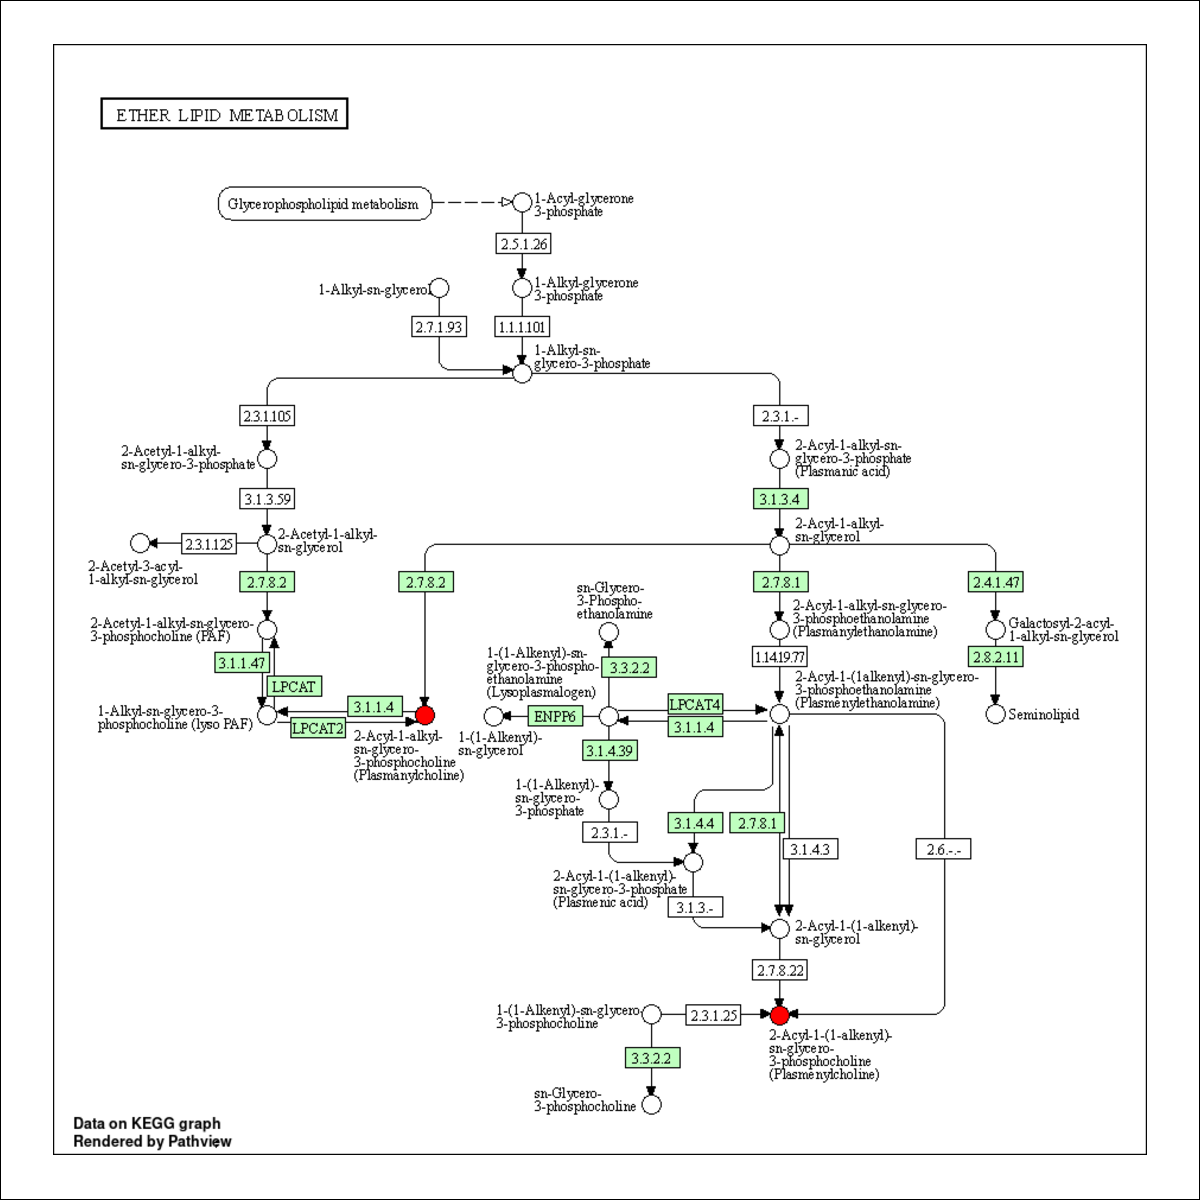
\includegraphics[width=1\linewidth,]{LipidSigR_files/figure-latex/unnamed-chunk-35-1} 

}

\caption{An example of KEGG pathway}\label{fig:unnamed-chunk-35}
\end{figure}

\textbackslash begin\{kframe\}

\hypertarget{lipid-characteristics-analysis}{%
\subsection{Lipid characteristics analysis}\label{lipid-characteristics-analysis}}

After lipid species analysis, now let's move on to another main analysis of the Differential expression section -- \textbf{`Lipid Characteristics Analysis'}. The massive degree of structural diversity of lipids contributes to the functional variety of lipids. The characteristics can range from subtle variance (i.e.~the number of a double bond in the fatty acid) to major change (i.e.~diverse backbones). In this section, lipid species are categorized and summarized into a new lipid expression table according to two selected lipid characteristics, then conducted differential expressed analysis. Samples are divided into two groups based on the input `Group Information' table.

\hypertarget{sec:DE-char}{%
\subsubsection{Differentially expressed analysis}\label{sec:DE-char}}

In differentially expressed analysis, we are going to conduct two procedures of analysis - first is \textbf{`Characteristics'} and then \textbf{`Subgroup of characteristics'}. \textbf{`Characteristics'} is based on the first selected `characteristics' while \textbf{`Subgroup of characteristics'} is the subgroup analysis of the previous section.

\begin{Shaded}
\begin{Highlighting}[]
\CommentTok{# get lipid characteristics}
\NormalTok{char_var <-}\StringTok{ }\KeywordTok{colnames}\NormalTok{(lipid_char_table)[}\OperatorTok{-}\DecValTok{1}\NormalTok{]}
\CommentTok{# aggregated(sum) expression data by selected characteristics}
\NormalTok{exp_data_Spe2Char <-}\StringTok{ }\KeywordTok{Species2Char}\NormalTok{(exp_data, lipid_char_table,}
                                  \DataTypeTok{char_var =}\NormalTok{ char_var[}\DecValTok{4}\NormalTok{])}
\CommentTok{# data processing of exp_data (without log10 transformation)}
\NormalTok{exp_transform_non_log <-}\StringTok{ }\KeywordTok{data_process}\NormalTok{(exp_data_Spe2Char,}
                                      \DataTypeTok{exclude_var_missing=}\OtherTok{TRUE}\NormalTok{,}
                                      \DataTypeTok{missing_pct_limit=}\DecValTok{50}\NormalTok{,}
                                      \DataTypeTok{replace_zero=}\OtherTok{TRUE}\NormalTok{,}
                                      \DataTypeTok{zero2what=}\StringTok{'min'}\NormalTok{, }\DataTypeTok{xmin=}\FloatTok{0.5}\NormalTok{,}
                                      \DataTypeTok{replace_NA=}\OtherTok{TRUE}\NormalTok{, }\DataTypeTok{NA2what=}\StringTok{'min'}\NormalTok{,}
                                      \DataTypeTok{ymin=}\FloatTok{0.5}\NormalTok{, }\DataTypeTok{pct_transform=}\OtherTok{TRUE}\NormalTok{,}
                                      \DataTypeTok{data_transform=}\OtherTok{FALSE}\NormalTok{,}
                                      \DataTypeTok{trans_type=}\StringTok{'log'}\NormalTok{,}
                                      \DataTypeTok{centering=}\OtherTok{FALSE}\NormalTok{, }\DataTypeTok{scaling=}\OtherTok{FALSE}\NormalTok{)}
\CommentTok{# conduct deferentially expressed of lipid characters}
\NormalTok{DE_char_result <-}\StringTok{ }\KeywordTok{DE_char_2}\NormalTok{(exp_transform_non_log, }\DataTypeTok{data_transform=}\OtherTok{TRUE}\NormalTok{,}
                            \DataTypeTok{group_info =}\NormalTok{ group_info, }\DataTypeTok{paired=}\OtherTok{FALSE}\NormalTok{,}
                            \DataTypeTok{sig_pvalue=}\FloatTok{0.05}\NormalTok{, }\DataTypeTok{sig_FC=}\DecValTok{2}\NormalTok{,}
                            \DataTypeTok{insert_ref_group=}\OtherTok{NULL}\NormalTok{, }\DataTypeTok{ref_group=}\OtherTok{NULL}\NormalTok{)}

\CommentTok{# view result: data frame of expression}
\KeywordTok{head}\NormalTok{(DE_char_result}\OperatorTok{$}\NormalTok{DE_char_exp_data[, }\DecValTok{1}\OperatorTok{:}\DecValTok{5}\NormalTok{], }\DecValTok{5}\NormalTok{)}
\CommentTok{##   totallength  control_01  control_02  control_03  control_04}
\CommentTok{## 1          14 0.007876691 0.005188040 0.002007919 0.002262715}
\CommentTok{## 2          16 0.614686226 0.371303913 0.440362404 0.360532543}
\CommentTok{## 3          18 0.499222531 0.340597404 0.336071017 0.233617647}
\CommentTok{## 4          20 0.138269347 0.045272091 0.047786065 0.057898780}
\CommentTok{## 5          22 0.021905258 0.004618018 0.011122576 0.007643132}

\CommentTok{# view result: data frame of statistical analysis}
\KeywordTok{head}\NormalTok{(DE_char_result}\OperatorTok{$}\NormalTok{DE_char_table_all[, }\DecValTok{1}\OperatorTok{:}\DecValTok{5}\NormalTok{], }\DecValTok{5}\NormalTok{)}
\CommentTok{##   totallength        method anova_pvalue post_hoc_test   mean_ctrl}
\CommentTok{## 1          14 two-way anova 4.344857e-05        t.test 0.005739745}
\CommentTok{## 2          16 two-way anova 4.344857e-05        t.test 0.551457134}
\CommentTok{## 3          18 two-way anova 4.344857e-05        t.test 0.527247670}
\CommentTok{## 4          20 two-way anova 4.344857e-05        t.test 0.096587704}
\CommentTok{## 5          22 two-way anova 4.344857e-05        t.test 0.014645490}

\CommentTok{# view result: data frame with value of the continuous lipid characteristics}
\KeywordTok{head}\NormalTok{(DE_char_result}\OperatorTok{$}\NormalTok{DE_char_combined_table[, }\DecValTok{1}\OperatorTok{:}\DecValTok{5}\NormalTok{])}
\CommentTok{##         totallength control_01 control_02 control_03 control_04}
\CommentTok{## 1 totallength_index   41.41296   41.25918   40.19358   41.21941}

\CommentTok{# view result: data frame with statistics of t.test}
\KeywordTok{head}\NormalTok{(DE_char_result}\OperatorTok{$}\NormalTok{DE_char_combine_result_table[, }\DecValTok{1}\OperatorTok{:}\DecValTok{5}\NormalTok{])}
\CommentTok{##         totallength method mean_ctrl   sd_ctrl mean_exp}
\CommentTok{## 1 totallength_index t.test  40.68546 0.4939548 41.02902}
\end{Highlighting}
\end{Shaded}

\begin{Shaded}
\begin{Highlighting}[]
\CommentTok{# view result: bar plot of split_class}
\NormalTok{DE_char_result}\OperatorTok{$}\NormalTok{DE_char_barplot }
\end{Highlighting}
\end{Shaded}

\label{fig:unnamed-chunk-36}The results of `Characteristics' analysis in the first section - bar plot

\begin{Shaded}
\begin{Highlighting}[]
\CommentTok{# view result: sqrt-scaled bar plot of split_class}
\NormalTok{DE_char_result}\OperatorTok{$}\NormalTok{DE_char_barplot_sqrt}
\end{Highlighting}
\end{Shaded}

\label{fig:unnamed-chunk-37}The results of `Characteristics' analysis in the first section - sqrt-scaled bar plot

\begin{Shaded}
\begin{Highlighting}[]
\CommentTok{# view result: line plot of split_class}
\NormalTok{DE_char_result}\OperatorTok{$}\NormalTok{DE_char_trendplot  }
\end{Highlighting}
\end{Shaded}

\label{fig:unnamed-chunk-38}The results of `Characteristics' analysis in the first section - line plot

\begin{Shaded}
\begin{Highlighting}[]
\CommentTok{# view result: sqrt-scaled line plot of split_class}
\NormalTok{DE_char_result}\OperatorTok{$}\NormalTok{DE_char_trendplot_sqrt  }
\end{Highlighting}
\end{Shaded}

\label{fig:unnamed-chunk-39}The results of `Characteristics' analysis in the first section - sqrt-scaled line plot

\begin{Shaded}
\begin{Highlighting}[]
\CommentTok{# view result: box plot of split_class}
\NormalTok{DE_char_result}\OperatorTok{$}\NormalTok{DE_char_boxplot  }
\end{Highlighting}
\end{Shaded}

\label{fig:unnamed-chunk-40}The results of `Characteristics' analysis in the first section - box plot

In the \textbf{`Subgroup of characteristics'}, besides the selected characteristic in first section defined by parameter \texttt{char\_var}, we can further choose another characteristic by parameter \texttt{split\_var} (e.g.~class). And then, analyzed results from the previous section are categorized by one of the subgroups (e.g.~PC) of the selected characteristic.

\begin{Shaded}
\begin{Highlighting}[]
\CommentTok{# get lipid characteristics}
\NormalTok{char_var <-}\StringTok{ }\KeywordTok{colnames}\NormalTok{(lipid_char_table)[}\OperatorTok{-}\DecValTok{1}\NormalTok{]}
\CommentTok{# subgroup deferentially expressed of lipid characters}
\NormalTok{DE.sub.char}\FloatTok{.2}\NormalTok{ <-}\StringTok{ }\KeywordTok{DE_sub_char_2}\NormalTok{(exp_data, }\DataTypeTok{data_transform=}\OtherTok{TRUE}\NormalTok{,}
                               \DataTypeTok{lipid_char_table=}\NormalTok{lipid_char_table,}
                               \DataTypeTok{split_var =}\NormalTok{ char_var[}\DecValTok{1}\NormalTok{],}
                               \DataTypeTok{char_var =}\NormalTok{ char_var[}\DecValTok{4}\NormalTok{],}
                               \DataTypeTok{group_info =}\NormalTok{ group_info,}
                               \DataTypeTok{paired=}\OtherTok{FALSE}\NormalTok{, }\DataTypeTok{sig_pvalue=}\FloatTok{0.05}\NormalTok{,}
                               \DataTypeTok{sig_FC=}\DecValTok{2}\NormalTok{, }\DataTypeTok{exclude_var_missing=}\OtherTok{TRUE}\NormalTok{,}
                               \DataTypeTok{missing_pct_limit=}\DecValTok{50}\NormalTok{,}
                               \DataTypeTok{replace_zero=}\OtherTok{TRUE}\NormalTok{, }\DataTypeTok{zero2what=}\StringTok{'min'}\NormalTok{,}
                               \DataTypeTok{xmin=}\FloatTok{0.5}\NormalTok{, }\DataTypeTok{replace_NA=}\OtherTok{TRUE}\NormalTok{,}
                               \DataTypeTok{NA2what=}\StringTok{'min'}\NormalTok{, }\DataTypeTok{ymin=}\FloatTok{0.5}\NormalTok{,}
                               \DataTypeTok{pct_transform=}\OtherTok{TRUE}\NormalTok{, }\DataTypeTok{trans_type=}\StringTok{'log'}\NormalTok{,}
                               \DataTypeTok{centering=}\OtherTok{FALSE}\NormalTok{, }\DataTypeTok{scaling=}\OtherTok{FALSE}\NormalTok{)}
\CommentTok{# get class of characteristics}
\NormalTok{char.class <-}\StringTok{ }\KeywordTok{unique}\NormalTok{(DE.sub.char}\FloatTok{.2}\NormalTok{[[}\DecValTok{2}\NormalTok{]][}\DecValTok{1}\NormalTok{])}
\CommentTok{# visualize subgroup deferentially expressed of lipid characters}
\NormalTok{sub_char_result <-}\StringTok{ }\KeywordTok{DE_sub_char_plot_2}\NormalTok{(DE.sub.char}\FloatTok{.2}\NormalTok{[[}\DecValTok{2}\NormalTok{]],}
\NormalTok{                                      DE.sub.char}\FloatTok{.2}\NormalTok{[[}\DecValTok{3}\NormalTok{]],}
                                      \DataTypeTok{group_info=}\NormalTok{group_info,}
                                      \DataTypeTok{char_var=}\NormalTok{char_var[}\DecValTok{4}\NormalTok{],}
                                      \DataTypeTok{split_var=}\NormalTok{char_var[}\DecValTok{1}\NormalTok{],}
                                      \DataTypeTok{split_class=}\NormalTok{char.class[}\DecValTok{5}\NormalTok{,],}
                                      \DataTypeTok{insert_ref_group=}\OtherTok{NULL}\NormalTok{, }\DataTypeTok{ref_group=}\OtherTok{NULL}\NormalTok{)}
\end{Highlighting}
\end{Shaded}

\begin{itemize}
\tightlist
\item
  \emph{Note: The star above the bar shows the significant difference of the specific subgroup of the selected characteristic between control and experimental groups.}
\end{itemize}

\begin{Shaded}
\begin{Highlighting}[]
\CommentTok{# view result: bar plot of split_class}
\NormalTok{sub_char_result[[}\DecValTok{1}\NormalTok{]]  }
\end{Highlighting}
\end{Shaded}

\label{fig:unnamed-chunk-41}The results of `Subgroup of characteristics' analysis in the second section - bar plot

\begin{Shaded}
\begin{Highlighting}[]
\CommentTok{# view result: sqrt-scaled bar plot of split_class}
\NormalTok{sub_char_result[[}\DecValTok{4}\NormalTok{]]}
\end{Highlighting}
\end{Shaded}

\label{fig:unnamed-chunk-42}The results of `Subgroup of characteristics' analysis in the second section - sqrt-scaled bar plot

\begin{Shaded}
\begin{Highlighting}[]
\CommentTok{# view result: line plot of split_class}
\NormalTok{sub_char_result[[}\DecValTok{2}\NormalTok{]]}
\end{Highlighting}
\end{Shaded}

\label{fig:unnamed-chunk-43}The results of `Subgroup of characteristics' analysis in the second section - line plot

\begin{Shaded}
\begin{Highlighting}[]
\CommentTok{# view result: sqrt-scaled line plot of split_class}
\NormalTok{sub_char_result[[}\DecValTok{5}\NormalTok{]] }
\end{Highlighting}
\end{Shaded}

\label{fig:unnamed-chunk-44}The results of `Subgroup of characteristics' analysis in the second section - sqrt-scaled line plot

\begin{Shaded}
\begin{Highlighting}[]
\CommentTok{# view result: box plot of split_class}
\NormalTok{sub_char_result[[}\DecValTok{3}\NormalTok{]] }
\end{Highlighting}
\end{Shaded}

\label{fig:unnamed-chunk-45}The results of `Subgroup of characteristics' analysis in the second section - box plot

\hypertarget{dimensionality-reduction}{%
\subsubsection{Dimensionality reduction}\label{dimensionality-reduction}}

Dimensionality reduction is common when dealing with large numbers of observations and/or large numbers of variables in lipids analysis. It transforms data from a high-dimensional space into a low-dimensional space to retain vital properties of the original data and close to its intrinsic dimension. Here, we provide 4 dimensionality reduction methods, namely, PCA, t-SNE, UMAP, and PLS-DA. For the detailed information of the former three methods, please refer to Section \ref{DimensionReduce}.

\hypertarget{pca-principal-component-analysis-1}{%
\paragraph{PCA (Principal component analysis)}\label{pca-principal-component-analysis-1}}

PCA is an unsupervised linear dimensionality reduction and data visualization technique for high dimensional data, which tries to preserve the global structure of the data. For detailed information of PCA, please refer to Section \ref{PCA}.

\begin{Shaded}
\begin{Highlighting}[]
\CommentTok{# get lipid characteristics}
\NormalTok{char_var <-}\StringTok{ }\KeywordTok{colnames}\NormalTok{(lipid_char_table)[}\OperatorTok{-}\DecValTok{1}\NormalTok{]}
\CommentTok{# sum expression data by selected characteristics}
\NormalTok{exp_data_Spe2Char <-}\StringTok{ }\KeywordTok{Species2Char}\NormalTok{(exp_data, lipid_char_table,}
                                  \DataTypeTok{char_var =}\NormalTok{ char_var[}\DecValTok{4}\NormalTok{])}
\CommentTok{# data processing of exp_data_Spe2Char}
\NormalTok{exp_transform_class <-}\StringTok{ }\KeywordTok{data_process}\NormalTok{(exp_data_Spe2Char, }
                                    \DataTypeTok{exclude_var_missing=}\OtherTok{TRUE}\NormalTok{, }
                                    \DataTypeTok{missing_pct_limit=}\DecValTok{50}\NormalTok{, }\DataTypeTok{replace_zero=}\OtherTok{TRUE}\NormalTok{,}
                                    \DataTypeTok{zero2what=}\StringTok{'NA'}\NormalTok{, }\DataTypeTok{xmin=}\FloatTok{0.5}\NormalTok{, }\DataTypeTok{replace_NA=}\OtherTok{TRUE}\NormalTok{,}
                                    \DataTypeTok{NA2what=}\StringTok{'min'}\NormalTok{, }\DataTypeTok{ymin=}\FloatTok{0.5}\NormalTok{, }
                                    \DataTypeTok{pct_transform=}\OtherTok{TRUE}\NormalTok{,}
                                    \DataTypeTok{data_transform=}\OtherTok{TRUE}\NormalTok{, }\DataTypeTok{trans_type=}\StringTok{'log'}\NormalTok{,}
                                    \DataTypeTok{centering=}\OtherTok{FALSE}\NormalTok{, }\DataTypeTok{scaling=}\OtherTok{FALSE}\NormalTok{)}
\CommentTok{# data processing of exp_data (without log10 transformation)}
\NormalTok{exp_transform_non_log <-}\StringTok{ }\KeywordTok{data_process}\NormalTok{(exp_data_Spe2Char,}
                                      \DataTypeTok{exclude_var_missing=}\OtherTok{TRUE}\NormalTok{,}
                                      \DataTypeTok{missing_pct_limit=}\DecValTok{50}\NormalTok{,}
                                      \DataTypeTok{replace_zero=}\OtherTok{TRUE}\NormalTok{,}
                                      \DataTypeTok{zero2what=}\StringTok{'min'}\NormalTok{, }\DataTypeTok{xmin=}\FloatTok{0.5}\NormalTok{,}
                                      \DataTypeTok{replace_NA=}\OtherTok{TRUE}\NormalTok{, }\DataTypeTok{NA2what=}\StringTok{'min'}\NormalTok{,}
                                      \DataTypeTok{ymin=}\FloatTok{0.5}\NormalTok{, }\DataTypeTok{pct_transform=}\OtherTok{TRUE}\NormalTok{,}
                                      \DataTypeTok{data_transform=}\OtherTok{FALSE}\NormalTok{,}
                                      \DataTypeTok{trans_type=}\StringTok{'log'}\NormalTok{,}
                                      \DataTypeTok{centering=}\OtherTok{FALSE}\NormalTok{, }\DataTypeTok{scaling=}\OtherTok{FALSE}\NormalTok{)}
\CommentTok{# filter significant lipid characteristics}
\NormalTok{DE_char_table_sig <-}\StringTok{ }\KeywordTok{DE_char_2}\NormalTok{(exp_transform_non_log,}
                               \DataTypeTok{data_transform=}\OtherTok{TRUE}\NormalTok{,}
                               \DataTypeTok{group_info =}\NormalTok{ group_info,}
                               \DataTypeTok{paired=}\OtherTok{FALSE}\NormalTok{, }\DataTypeTok{sig_pvalue=}\FloatTok{0.05}\NormalTok{,}
                               \DataTypeTok{sig_FC=}\DecValTok{2}\NormalTok{)}\OperatorTok{$}\NormalTok{DE_char_table_all }\OperatorTok\StringTok{ }
\StringTok{                               }\KeywordTok{filter}\NormalTok{(sig}\OperatorTok{==}\StringTok{"yes"}\NormalTok{)}
\CommentTok{# conduct PCA}
\NormalTok{DEchar_PCA <-}\StringTok{ }\KeywordTok{PCA}\NormalTok{(exp_transform_class, }\DataTypeTok{group_info =}\NormalTok{ group_info,}
                  \DataTypeTok{sig_feature =}\NormalTok{ DE_char_table_sig[,}\DecValTok{1}\NormalTok{],}
                  \DataTypeTok{scaling=}\OtherTok{TRUE}\NormalTok{, }\DataTypeTok{centering=}\OtherTok{TRUE}\NormalTok{,}
                  \DataTypeTok{cluster_method=}\StringTok{'kmeans'}\NormalTok{,}
                  \DataTypeTok{group_num=}\DecValTok{2}\NormalTok{, }\DataTypeTok{var1 =} \OtherTok{NULL}\NormalTok{, }\DataTypeTok{var2 =} \OtherTok{NULL}\NormalTok{,}
                  \DataTypeTok{insert_ref_group=}\OtherTok{NULL}\NormalTok{, }\DataTypeTok{ref_group=}\OtherTok{NULL}\NormalTok{,}
                  \DataTypeTok{n_PC=}\KeywordTok{c}\NormalTok{(}\DecValTok{1}\NormalTok{,}\DecValTok{2}\NormalTok{), }\DataTypeTok{top_n_feature=}\DecValTok{10}\NormalTok{)}

\CommentTok{# view result: PCA prcomp}
\KeywordTok{head}\NormalTok{(DEchar_PCA[[}\DecValTok{1}\NormalTok{]], }\DecValTok{2}\NormalTok{)}
\CommentTok{## $sdev}
\CommentTok{## [1] 1.6953108 0.2786763 0.2196837}
\CommentTok{## }
\CommentTok{## $rotation}
\CommentTok{##           PC1        PC2        PC3}
\CommentTok{## 48 -0.5744300  0.8103231 -0.1157871}
\CommentTok{## 50 -0.5780849 -0.5017458 -0.6434819}
\CommentTok{## 51 -0.5795240 -0.3027006  0.7566534}

\CommentTok{# view result: data frame of PCA rotated data}
\KeywordTok{head}\NormalTok{(DEchar_PCA[[}\DecValTok{2}\NormalTok{]][,}\DecValTok{1}\OperatorTok{:}\DecValTok{5}\NormalTok{], }\DecValTok{5}\NormalTok{)}
\CommentTok{##            sample_name group        PC1         PC2         PC3}
\CommentTok{## control_01  control_01     2 -0.5466139 -0.12594152  0.12327983}
\CommentTok{## control_02  control_02     2 -1.3869805  0.13744289 -0.03504498}
\CommentTok{## control_03  control_03     1  2.5648862  0.01778046 -0.11647110}
\CommentTok{## control_04  control_04     2 -0.3094606 -0.25223171 -0.02916247}
\CommentTok{## control_05  control_05     1  1.8308181  0.23114389  0.20304546}

\CommentTok{# view result: data frame of PCA contribution table}
\KeywordTok{head}\NormalTok{(DEchar_PCA[[}\DecValTok{3}\NormalTok{]])}
\CommentTok{##    feature      PC1       PC2       PC3}
\CommentTok{## 48      48 32.99698 65.662350  1.340665}
\CommentTok{## 50      50 33.41821 25.174885 41.406901}
\CommentTok{## 51      51 33.58480  9.162764 57.252434}
\end{Highlighting}
\end{Shaded}

\begin{Shaded}
\begin{Highlighting}[]
\CommentTok{# view result: PCA plot }
\NormalTok{DEchar_PCA[[}\DecValTok{4}\NormalTok{]]  }
\end{Highlighting}
\end{Shaded}

\label{fig:unnamed-chunk-46}Results of PCA - PCA plot

\begin{Shaded}
\begin{Highlighting}[]
\CommentTok{# view result: scree plot}
\NormalTok{DEchar_PCA[[}\DecValTok{5}\NormalTok{]]   }
\end{Highlighting}
\end{Shaded}

\label{fig:unnamed-chunk-47}Results of PCA - scree plot

\begin{Shaded}
\begin{Highlighting}[]
\CommentTok{# view result: bar plot of features contribution}
\NormalTok{DEchar_PCA[[}\DecValTok{6}\NormalTok{]]}
\end{Highlighting}
\end{Shaded}

\label{fig:unnamed-chunk-48}Results of PCA - bar plot

\begin{Shaded}
\begin{Highlighting}[]
\CommentTok{# view result: correlation circle plot of variables}
\NormalTok{DEchar_PCA[[}\DecValTok{7}\NormalTok{]]}
\end{Highlighting}
\end{Shaded}

\label{fig:unnamed-chunk-49}Results of PCA - correlation circle plot

\hypertarget{t-sne-t-distributed-stochastic-neighbour-embedding-1}{%
\paragraph{t-SNE (t-distributed stochastic neighbour embedding)}\label{t-sne-t-distributed-stochastic-neighbour-embedding-1}}

t-Distributed Stochastic Neighbour Embedding (t-SNE) is an unsupervised non-linear dimensionality reduction technique that tries to retain the local structure(cluster) of data when visualising the high-dimensional datasets. For detailed information of t-SNE, please refer to Section \ref{t-SNE}.

\begin{Shaded}
\begin{Highlighting}[]
\CommentTok{# get lipid characteristics}
\NormalTok{char_var <-}\StringTok{ }\KeywordTok{colnames}\NormalTok{(lipid_char_table)[}\OperatorTok{-}\DecValTok{1}\NormalTok{]}
\CommentTok{# sum expression data by selected characteristics}
\NormalTok{exp_data_Spe2Char <-}\StringTok{ }\KeywordTok{Species2Char}\NormalTok{(exp_data, lipid_char_table,}
                                  \DataTypeTok{char_var =}\NormalTok{ char_var[}\DecValTok{4}\NormalTok{])}
\CommentTok{# data processing of exp_data_Spe2Char}
\NormalTok{exp_transform_class <-}\StringTok{ }\KeywordTok{data_process}\NormalTok{(exp_data_Spe2Char, }
                                    \DataTypeTok{exclude_var_missing=}\OtherTok{TRUE}\NormalTok{,}
                                    \DataTypeTok{missing_pct_limit=}\DecValTok{50}\NormalTok{, }\DataTypeTok{replace_zero=}\OtherTok{TRUE}\NormalTok{,}
                                    \DataTypeTok{zero2what=}\StringTok{'NA'}\NormalTok{, }\DataTypeTok{xmin=}\FloatTok{0.5}\NormalTok{, }\DataTypeTok{replace_NA=}\OtherTok{TRUE}\NormalTok{,}
                                    \DataTypeTok{NA2what=}\StringTok{'min'}\NormalTok{, }\DataTypeTok{ymin=}\FloatTok{0.5}\NormalTok{, }
                                    \DataTypeTok{pct_transform=}\OtherTok{TRUE}\NormalTok{,}
                                    \DataTypeTok{data_transform=}\OtherTok{TRUE}\NormalTok{, }\DataTypeTok{trans_type=}\StringTok{'log'}\NormalTok{,}
                                    \DataTypeTok{centering=}\OtherTok{FALSE}\NormalTok{, }\DataTypeTok{scaling=}\OtherTok{FALSE}\NormalTok{)}
\CommentTok{# data processing of exp_data (without log10 transformation)}
\NormalTok{exp_transform_non_log <-}\StringTok{ }\KeywordTok{data_process}\NormalTok{(exp_data_Spe2Char,}
                                      \DataTypeTok{exclude_var_missing=}\OtherTok{TRUE}\NormalTok{,}
                                      \DataTypeTok{missing_pct_limit=}\DecValTok{50}\NormalTok{,}
                                      \DataTypeTok{replace_zero=}\OtherTok{TRUE}\NormalTok{,}
                                      \DataTypeTok{zero2what=}\StringTok{'min'}\NormalTok{, }\DataTypeTok{xmin=}\FloatTok{0.5}\NormalTok{,}
                                      \DataTypeTok{replace_NA=}\OtherTok{TRUE}\NormalTok{, }\DataTypeTok{NA2what=}\StringTok{'min'}\NormalTok{,}
                                      \DataTypeTok{ymin=}\FloatTok{0.5}\NormalTok{, }\DataTypeTok{pct_transform=}\OtherTok{TRUE}\NormalTok{,}
                                      \DataTypeTok{data_transform=}\OtherTok{FALSE}\NormalTok{,}
                                      \DataTypeTok{trans_type=}\StringTok{'log'}\NormalTok{,}
                                      \DataTypeTok{centering=}\OtherTok{FALSE}\NormalTok{, }\DataTypeTok{scaling=}\OtherTok{FALSE}\NormalTok{)}
\CommentTok{# filter significant lipid characteristics}
\NormalTok{DE_char_table_sig <-}\StringTok{ }\KeywordTok{DE_char_2}\NormalTok{(exp_transform_non_log,}
                               \DataTypeTok{data_transform=}\OtherTok{TRUE}\NormalTok{,}
                               \DataTypeTok{group_info =}\NormalTok{ group_info,}
                               \DataTypeTok{paired=}\OtherTok{FALSE}\NormalTok{, }\DataTypeTok{sig_pvalue=}\FloatTok{0.05}\NormalTok{,}
                               \DataTypeTok{sig_FC=}\DecValTok{2}\NormalTok{)}\OperatorTok{$}\NormalTok{DE_char_table_all }\OperatorTok\StringTok{ }
\StringTok{                               }\KeywordTok{filter}\NormalTok{(sig}\OperatorTok{==}\StringTok{"yes"}\NormalTok{)}
\CommentTok{# conduct t-SNE}
\NormalTok{DEchar_tsne <-}\StringTok{ }\KeywordTok{tsne}\NormalTok{(exp_transform_class, }\DataTypeTok{group_info =}\NormalTok{ group_info,}
                    \DataTypeTok{sig_feature=}\NormalTok{DE_char_table_sig[,}\DecValTok{1}\NormalTok{],}
                    \DataTypeTok{pca=}\OtherTok{TRUE}\NormalTok{, }\DataTypeTok{perplexity=}\DecValTok{5}\NormalTok{, }\DataTypeTok{max_iter=}\DecValTok{500}\NormalTok{,}
                    \DataTypeTok{cluster_method=}\StringTok{'kmeans'}\NormalTok{, }\DataTypeTok{group_num=}\DecValTok{2}\NormalTok{,}
                    \DataTypeTok{var1 =} \StringTok{'euclidean'}\NormalTok{, }\DataTypeTok{var2=}\OtherTok{NULL}\NormalTok{,}
                    \DataTypeTok{insert_ref_group=}\OtherTok{NULL}\NormalTok{, }\DataTypeTok{ref_group=}\OtherTok{NULL}\NormalTok{)}
\CommentTok{## Performing PCA}
\CommentTok{## Read the 23 x 3 data matrix successfully!}
\CommentTok{## OpenMP is working. 1 threads.}
\CommentTok{## Using no_dims = 2, perplexity = 5.000000, and theta = 0.000000}
\CommentTok{## Computing input similarities...}
\CommentTok{## Symmetrizing...}
\CommentTok{## Done in 0.00 seconds!}
\CommentTok{## Learning embedding...}
\CommentTok{## Iteration 50: error is 57.688290 (50 iterations in 0.00 seconds)}
\CommentTok{## Iteration 100: error is 59.141604 (50 iterations in 0.00 seconds)}
\CommentTok{## Iteration 150: error is 61.711247 (50 iterations in 0.00 seconds)}
\CommentTok{## Iteration 200: error is 52.980025 (50 iterations in 0.00 seconds)}
\CommentTok{## Iteration 250: error is 50.493041 (50 iterations in 0.00 seconds)}
\CommentTok{## Iteration 300: error is 1.471355 (50 iterations in 0.00 seconds)}
\CommentTok{## Iteration 350: error is 0.418058 (50 iterations in 0.00 seconds)}
\CommentTok{## Iteration 400: error is 0.212979 (50 iterations in 0.00 seconds)}
\CommentTok{## Iteration 450: error is 0.187534 (50 iterations in 0.00 seconds)}
\CommentTok{## Iteration 500: error is 0.164958 (50 iterations in 0.00 seconds)}
\CommentTok{## Fitting performed in 0.00 seconds.}

\CommentTok{# view result: data frame of t-SNE data}
\KeywordTok{head}\NormalTok{(DEchar_tsne[[}\DecValTok{1}\NormalTok{]], }\DecValTok{5}\NormalTok{)}
\CommentTok{##   sample_name group     tsne1      tsne2}
\CommentTok{## 1  control_01     2 -47.14225  45.774040}
\CommentTok{## 2  control_02     1 -55.39699 -39.547783}
\CommentTok{## 3  control_03     2  89.94977   6.156967}
\CommentTok{## 4  control_04     2 -34.56940  45.047167}
\CommentTok{## 5  control_05     2  64.42728  -0.643910}
\end{Highlighting}
\end{Shaded}

\begin{Shaded}
\begin{Highlighting}[]
\CommentTok{# view result: t-SNE plot}
\NormalTok{DEchar_tsne[[}\DecValTok{2}\NormalTok{]]  }
\end{Highlighting}
\end{Shaded}

\label{fig:unnamed-chunk-50}t-SNE plot

\hypertarget{umap-uniform-manifold-approximation-and-projection-1}{%
\paragraph{UMAP (Uniform Manifold Approximation and Projection)}\label{umap-uniform-manifold-approximation-and-projection-1}}

UMAP using a nonlinear dimensionality reduction method, Manifold learning, which effectively visualizing clusters or groups of data points and their relative proximities. For detailed information of UMAP, please refer to Section \ref{UMAP}.

\begin{Shaded}
\begin{Highlighting}[]
\CommentTok{# get lipid characteristics}
\NormalTok{char_var <-}\StringTok{ }\KeywordTok{colnames}\NormalTok{(lipid_char_table)[}\OperatorTok{-}\DecValTok{1}\NormalTok{]}
\CommentTok{# sum expression data by selected characteristics}
\NormalTok{exp_data_Spe2Char <-}\StringTok{ }\KeywordTok{Species2Char}\NormalTok{(exp_data, lipid_char_table,}
                                  \DataTypeTok{char_var =}\NormalTok{ char_var[}\DecValTok{4}\NormalTok{])}
\CommentTok{# data processing of exp_data_Spe2Char}
\NormalTok{exp_transform_class <-}\StringTok{ }\KeywordTok{data_process}\NormalTok{(exp_data_Spe2Char, }
                                    \DataTypeTok{exclude_var_missing=}\OtherTok{TRUE}\NormalTok{,}
                                    \DataTypeTok{missing_pct_limit=}\DecValTok{50}\NormalTok{, }\DataTypeTok{replace_zero=}\OtherTok{TRUE}\NormalTok{,}
                                    \DataTypeTok{zero2what=}\StringTok{'NA'}\NormalTok{, }\DataTypeTok{xmin=}\FloatTok{0.5}\NormalTok{, }\DataTypeTok{replace_NA=}\OtherTok{TRUE}\NormalTok{,}
                                    \DataTypeTok{NA2what=}\StringTok{'min'}\NormalTok{, }\DataTypeTok{ymin=}\FloatTok{0.5}\NormalTok{, }
                                    \DataTypeTok{pct_transform=}\OtherTok{TRUE}\NormalTok{,}
                                    \DataTypeTok{data_transform=}\OtherTok{TRUE}\NormalTok{, }\DataTypeTok{trans_type=}\StringTok{'log'}\NormalTok{,}
                                    \DataTypeTok{centering=}\OtherTok{FALSE}\NormalTok{, }\DataTypeTok{scaling=}\OtherTok{FALSE}\NormalTok{)}
\CommentTok{# data processing of exp_data (without log10 transformation)}
\NormalTok{exp_transform_non_log <-}\StringTok{ }\KeywordTok{data_process}\NormalTok{(exp_data_Spe2Char,}
                                      \DataTypeTok{exclude_var_missing=}\OtherTok{TRUE}\NormalTok{,}
                                      \DataTypeTok{missing_pct_limit=}\DecValTok{50}\NormalTok{,}
                                      \DataTypeTok{replace_zero=}\OtherTok{TRUE}\NormalTok{,}
                                      \DataTypeTok{zero2what=}\StringTok{'min'}\NormalTok{, }\DataTypeTok{xmin=}\FloatTok{0.5}\NormalTok{,}
                                      \DataTypeTok{replace_NA=}\OtherTok{TRUE}\NormalTok{, }\DataTypeTok{NA2what=}\StringTok{'min'}\NormalTok{,}
                                      \DataTypeTok{ymin=}\FloatTok{0.5}\NormalTok{, }\DataTypeTok{pct_transform=}\OtherTok{TRUE}\NormalTok{,}
                                      \DataTypeTok{data_transform=}\OtherTok{FALSE}\NormalTok{,}
                                      \DataTypeTok{trans_type=}\StringTok{'log'}\NormalTok{,}
                                      \DataTypeTok{centering=}\OtherTok{FALSE}\NormalTok{, }\DataTypeTok{scaling=}\OtherTok{FALSE}\NormalTok{)}
\CommentTok{# filter significant lipid characteristics}
\NormalTok{DE_char_table_sig <-}\StringTok{ }\KeywordTok{DE_char_2}\NormalTok{(exp_transform_non_log,}
                               \DataTypeTok{data_transform=}\OtherTok{TRUE}\NormalTok{,}
                               \DataTypeTok{group_info =}\NormalTok{ group_info,}
                               \DataTypeTok{paired=}\OtherTok{FALSE}\NormalTok{, }\DataTypeTok{sig_pvalue=}\FloatTok{0.05}\NormalTok{,}
                               \DataTypeTok{sig_FC=}\DecValTok{2}\NormalTok{)}\OperatorTok{$}\NormalTok{DE_char_table_all }\OperatorTok\StringTok{ }
\StringTok{                               }\KeywordTok{filter}\NormalTok{(sig}\OperatorTok{==}\StringTok{"yes"}\NormalTok{)}
\CommentTok{# conduct UMAP}
\NormalTok{DEchar_UMAP <-}\StringTok{ }\KeywordTok{UMAP}\NormalTok{(exp_transform_class, }\DataTypeTok{group_info =}\NormalTok{ group_info,}
                    \DataTypeTok{sig_feature =}\NormalTok{ DE_char_table_sig[,}\DecValTok{1}\NormalTok{],}
                    \DataTypeTok{n_neighbors=}\DecValTok{15}\NormalTok{, }\DataTypeTok{scale=}\OtherTok{TRUE}\NormalTok{, }\DataTypeTok{group_num=}\DecValTok{2}\NormalTok{,}
                    \DataTypeTok{metric =} \StringTok{'euclidean'}\NormalTok{,}
                    \DataTypeTok{cluster_method =} \StringTok{'kmeans'}\NormalTok{,}
                    \DataTypeTok{var1=}\OtherTok{NULL}\NormalTok{, }\DataTypeTok{var2=}\OtherTok{NULL}\NormalTok{,}
                    \DataTypeTok{insert_ref_group=}\OtherTok{NULL}\NormalTok{, }\DataTypeTok{ref_group=}\OtherTok{NULL}\NormalTok{)}

\CommentTok{# view result: data frame of UMAP data}
\KeywordTok{head}\NormalTok{(DEchar_UMAP[[}\DecValTok{1}\NormalTok{]], }\DecValTok{5}\NormalTok{)}
\CommentTok{##            sample_name group     UMAP-1     UMAP-2}
\CommentTok{## control_01  control_01     2 -0.5915072  0.7558721}
\CommentTok{## control_02  control_02     2 -1.4145067  0.4868656}
\CommentTok{## control_03  control_03     1  1.7309618 -1.9166599}
\CommentTok{## control_04  control_04     2  0.0135362  0.9845302}
\CommentTok{## control_05  control_05     1  1.4063492 -1.1956604}
\end{Highlighting}
\end{Shaded}

\begin{Shaded}
\begin{Highlighting}[]
\CommentTok{# view result: UMAP plot}
\NormalTok{DEchar_UMAP[[}\DecValTok{2}\NormalTok{]] }
\end{Highlighting}
\end{Shaded}

\label{fig:unnamed-chunk-51}UMAP plot

\hypertarget{pls-da-1}{%
\paragraph{PLS-DA}\label{pls-da-1}}

\begin{Shaded}
\begin{Highlighting}[]
\CommentTok{# get lipid characteristics}
\NormalTok{char_var <-}\StringTok{ }\KeywordTok{colnames}\NormalTok{(lipid_char_table)[}\OperatorTok{-}\DecValTok{1}\NormalTok{]}
\CommentTok{# sum expression data by selected characteristics}
\NormalTok{exp_data_Spe2Char <-}\StringTok{ }\KeywordTok{Species2Char}\NormalTok{(exp_data, lipid_char_table,}
                                  \DataTypeTok{char_var =}\NormalTok{ char_var[}\DecValTok{4}\NormalTok{])}
\CommentTok{# data processing of exp_data_Spe2Char}
\NormalTok{exp_transform_class <-}\StringTok{ }\KeywordTok{data_process}\NormalTok{(exp_data_Spe2Char, }
                                    \DataTypeTok{exclude_var_missing=}\OtherTok{TRUE}\NormalTok{,}
                                    \DataTypeTok{missing_pct_limit=}\DecValTok{50}\NormalTok{, }\DataTypeTok{replace_zero=}\OtherTok{TRUE}\NormalTok{,}
                                    \DataTypeTok{zero2what=}\StringTok{'NA'}\NormalTok{, }\DataTypeTok{xmin=}\FloatTok{0.5}\NormalTok{, }\DataTypeTok{replace_NA=}\OtherTok{TRUE}\NormalTok{,}
                                    \DataTypeTok{NA2what=}\StringTok{'min'}\NormalTok{, }\DataTypeTok{ymin=}\FloatTok{0.5}\NormalTok{, }
                                    \DataTypeTok{pct_transform=}\OtherTok{TRUE}\NormalTok{,}
                                    \DataTypeTok{data_transform=}\OtherTok{TRUE}\NormalTok{, }\DataTypeTok{trans_type=}\StringTok{'log'}\NormalTok{,}
                                    \DataTypeTok{centering=}\OtherTok{FALSE}\NormalTok{, }\DataTypeTok{scaling=}\OtherTok{FALSE}\NormalTok{)}
\CommentTok{# data processing of exp_data (without log10 transformation)}
\NormalTok{exp_transform_non_log <-}\StringTok{ }\KeywordTok{data_process}\NormalTok{(exp_data_Spe2Char,}
                                      \DataTypeTok{exclude_var_missing=}\OtherTok{TRUE}\NormalTok{,}
                                      \DataTypeTok{missing_pct_limit=}\DecValTok{50}\NormalTok{,}
                                      \DataTypeTok{replace_zero=}\OtherTok{TRUE}\NormalTok{,}
                                      \DataTypeTok{zero2what=}\StringTok{'min'}\NormalTok{, }\DataTypeTok{xmin=}\FloatTok{0.5}\NormalTok{,}
                                      \DataTypeTok{replace_NA=}\OtherTok{TRUE}\NormalTok{, }\DataTypeTok{NA2what=}\StringTok{'min'}\NormalTok{,}
                                      \DataTypeTok{ymin=}\FloatTok{0.5}\NormalTok{, }\DataTypeTok{pct_transform=}\OtherTok{TRUE}\NormalTok{,}
                                      \DataTypeTok{data_transform=}\OtherTok{FALSE}\NormalTok{,}
                                      \DataTypeTok{trans_type=}\StringTok{'log'}\NormalTok{,}
                                      \DataTypeTok{centering=}\OtherTok{FALSE}\NormalTok{, }\DataTypeTok{scaling=}\OtherTok{FALSE}\NormalTok{)}
\CommentTok{# filter significant lipid characteristics}
\NormalTok{DE_char_table_sig <-}\StringTok{ }\KeywordTok{DE_char_2}\NormalTok{(exp_transform_non_log,}
                               \DataTypeTok{data_transform=}\OtherTok{TRUE}\NormalTok{,}
                               \DataTypeTok{group_info =}\NormalTok{ group_info,}
                               \DataTypeTok{paired=}\OtherTok{FALSE}\NormalTok{, }\DataTypeTok{sig_pvalue=}\FloatTok{0.05}\NormalTok{,}
                               \DataTypeTok{sig_FC=}\DecValTok{2}\NormalTok{)}\OperatorTok{$}\NormalTok{DE_char_table_all }\OperatorTok\StringTok{ }
\StringTok{                               }\KeywordTok{filter}\NormalTok{(sig}\OperatorTok{==}\StringTok{"yes"}\NormalTok{)}
\CommentTok{# conduct PLSDA}
\NormalTok{DEchar_PLSDA <-}\StringTok{ }\KeywordTok{PLSDA}\NormalTok{(exp_transform_class, }\DataTypeTok{group_info =}\NormalTok{ group_info,}
                      \DataTypeTok{sig_feature=}\NormalTok{DE_char_table_sig[,}\DecValTok{1}\NormalTok{],}
                      \DataTypeTok{ncomp=}\DecValTok{2}\NormalTok{, }\DataTypeTok{scaling=}\OtherTok{TRUE}\NormalTok{, }\DataTypeTok{cluster_method=}\StringTok{'group_info'}\NormalTok{,}
                      \DataTypeTok{group_num =} \OtherTok{NULL}\NormalTok{, }\DataTypeTok{var1=}\OtherTok{NULL}\NormalTok{, }\DataTypeTok{var2=}\OtherTok{NULL}\NormalTok{,}
                      \DataTypeTok{insert_ref_group=}\OtherTok{NULL}\NormalTok{, }\DataTypeTok{ref_group=}\OtherTok{NULL}\NormalTok{)}

\CommentTok{# view result: data frame of sample variate}
\KeywordTok{head}\NormalTok{(DEchar_PLSDA[[}\DecValTok{1}\NormalTok{]], }\DecValTok{5}\NormalTok{)}
\CommentTok{##            sample_name group     PLSDA1      PLSDA2}
\CommentTok{## control_01  control_01  ctrl -0.5475526  0.03467860}
\CommentTok{## control_02  control_02  ctrl -1.3706971 -0.09832257}
\CommentTok{## control_03  control_03  ctrl  2.5472937  0.05654781}
\CommentTok{## control_04  control_04  ctrl -0.3303837  0.22597494}
\CommentTok{## control_05  control_05  ctrl  1.8520391 -0.30215285}

\CommentTok{# view result: data frame of sample loading}
\KeywordTok{head}\NormalTok{(DEchar_PLSDA[[}\DecValTok{2}\NormalTok{]])}
\CommentTok{##        PLSDA1     PLSDA2}
\CommentTok{## 48 -0.5109755 -0.6621155}
\CommentTok{## 50 -0.6520544  0.7141024}
\CommentTok{## 51 -0.5601153 -0.2272903}
\end{Highlighting}
\end{Shaded}

\begin{Shaded}
\begin{Highlighting}[]
\CommentTok{# view result: PLS-DA sample plot}
\NormalTok{DEchar_PLSDA[[}\DecValTok{3}\NormalTok{]]  }
\end{Highlighting}
\end{Shaded}

\label{fig:unnamed-chunk-52}PLS-DA sample plot

\begin{Shaded}
\begin{Highlighting}[]
\CommentTok{# view result: PLS-DA loading plot}
\NormalTok{DEchar_PLSDA[[}\DecValTok{4}\NormalTok{]]}
\end{Highlighting}
\end{Shaded}

\label{fig:unnamed-chunk-53}PLS-DA loading plot. In the PLS-DA loading plot, the distance to the center of the variables indicates the contribution of the variable. The value of the x-axis reveals the contribution of the variable to PLS-DA-1, whereas the value of the y-axis discloses the contribution of the variable to PLS-DA-2.

\hypertarget{hierarchical-clustering}{%
\subsubsection{Hierarchical clustering}\label{hierarchical-clustering}}

A new lipid expression table summed up from species is clustered and shown on the heatmap using hierarchical clustering.

\begin{Shaded}
\begin{Highlighting}[]
\CommentTok{# get lipid characteristics}
\NormalTok{char_var <-}\StringTok{ }\KeywordTok{colnames}\NormalTok{(lipid_char_table)[}\OperatorTok{-}\DecValTok{1}\NormalTok{]}
\CommentTok{# sum expression data by selected characteristics}
\NormalTok{exp_data_Spe2Char <-}\StringTok{ }\KeywordTok{Species2Char}\NormalTok{(exp_data, lipid_char_table,}
                                  \DataTypeTok{char_var =}\NormalTok{ char_var[}\DecValTok{4}\NormalTok{])}
\CommentTok{# data processing of exp_data_Spe2Char}
\NormalTok{exp_transform_class <-}\StringTok{ }\KeywordTok{data_process}\NormalTok{(exp_data_Spe2Char, }
                                    \DataTypeTok{exclude_var_missing=}\OtherTok{TRUE}\NormalTok{,}
                                    \DataTypeTok{missing_pct_limit=}\DecValTok{50}\NormalTok{, }\DataTypeTok{replace_zero=}\OtherTok{TRUE}\NormalTok{,}
                                    \DataTypeTok{replace_NA=}\OtherTok{TRUE}\NormalTok{,}\DataTypeTok{zero2what=}\StringTok{'NA'}\NormalTok{,}
                                    \DataTypeTok{NA2what=}\StringTok{'min'}\NormalTok{, }\DataTypeTok{pct_transform=}\OtherTok{TRUE}\NormalTok{, }
                                    \DataTypeTok{xmin=}\FloatTok{0.5}\NormalTok{, }\DataTypeTok{data_transform=}\OtherTok{TRUE}\NormalTok{, }
                                    \DataTypeTok{ymin=}\FloatTok{0.5}\NormalTok{, }\DataTypeTok{trans_type=}\StringTok{'log'}\NormalTok{, }
                                    \DataTypeTok{centering=}\OtherTok{FALSE}\NormalTok{, }\DataTypeTok{scaling=}\OtherTok{FALSE}\NormalTok{)}
\CommentTok{# data processing of exp_data (without log10 transformation)}
\NormalTok{exp_transform_non_log <-}\StringTok{ }\KeywordTok{data_process}\NormalTok{(exp_data_Spe2Char,}
                                      \DataTypeTok{exclude_var_missing=}\OtherTok{TRUE}\NormalTok{,}
                                      \DataTypeTok{missing_pct_limit=}\DecValTok{50}\NormalTok{,}
                                      \DataTypeTok{replace_zero=}\OtherTok{TRUE}\NormalTok{, }\DataTypeTok{zero2what=}\StringTok{'min'}\NormalTok{,}
                                      \DataTypeTok{xmin=}\FloatTok{0.5}\NormalTok{, }\DataTypeTok{replace_NA=}\OtherTok{TRUE}\NormalTok{, }\DataTypeTok{NA2what=}\StringTok{'min'}\NormalTok{,}
                                      \DataTypeTok{ymin=}\FloatTok{0.5}\NormalTok{, }\DataTypeTok{pct_transform=}\OtherTok{TRUE}\NormalTok{,}
                                      \DataTypeTok{data_transform=}\OtherTok{FALSE}\NormalTok{, }\DataTypeTok{trans_type=}\StringTok{'log'}\NormalTok{,}
                                      \DataTypeTok{centering=}\OtherTok{FALSE}\NormalTok{, }\DataTypeTok{scaling=}\OtherTok{FALSE}\NormalTok{)}
\CommentTok{# filter significant lipid characteristics}
\NormalTok{DE_char_table_sig <-}\StringTok{ }\KeywordTok{DE_char_2}\NormalTok{(exp_transform_non_log,}
                               \DataTypeTok{data_transform=}\OtherTok{TRUE}\NormalTok{, }\DataTypeTok{group_info =}\NormalTok{ group_info,}
                               \DataTypeTok{paired=}\OtherTok{FALSE}\NormalTok{, }\DataTypeTok{sig_pvalue=}\FloatTok{0.05}\NormalTok{, }\DataTypeTok{sig_FC=}\DecValTok{2}
\NormalTok{                              )}\OperatorTok{$}\NormalTok{DE_char_table_all }\OperatorTok\StringTok{ }\KeywordTok{filter}\NormalTok{(sig}\OperatorTok{==}\StringTok{"yes"}\NormalTok{)}
\CommentTok{# conduct hierarchical clustering}
\NormalTok{DEchar_Hcluster <-}\StringTok{ }\KeywordTok{Hclustering}\NormalTok{(exp_transform_class, DE_char_table_sig,}
\NormalTok{                               group_info, }\DataTypeTok{lipid_char_table=}\OtherTok{NULL}\NormalTok{, }
                               \DataTypeTok{char_var=}\OtherTok{NULL}\NormalTok{, }\DataTypeTok{distfun=}\StringTok{'pearson'}\NormalTok{, }
                               \DataTypeTok{hclustfun=}\StringTok{'complete'}\NormalTok{)}

\CommentTok{# view result: matrix of all lipid species heatmap}
\KeywordTok{head}\NormalTok{(DEchar_Hcluster}\OperatorTok{$}\NormalTok{all.lipid.data[, }\DecValTok{1}\OperatorTok{:}\DecValTok{5}\NormalTok{], }\DecValTok{5}\NormalTok{)}
\CommentTok{##       hfref3     ctrl5     ctrl7       ctrl6      ctrl8}
\CommentTok{## 36 1.8556987 0.5180388 0.5170678 -0.34186785 -0.2904855}
\CommentTok{## 14 0.5235378 0.5388503 0.4404471 -1.39383685  0.9335044}
\CommentTok{## 18 0.4053947 1.4803137 1.9614334  0.20197549  0.6085228}
\CommentTok{## 16 0.7343398 1.2327273 0.8511100  0.03909701  0.3186890}
\CommentTok{## 20 0.2614331 1.0882464 1.3247222  0.05499599  0.5322051}

\CommentTok{# view result: matrix of significant lipid species heatmap}
\KeywordTok{head}\NormalTok{(DEchar_Hcluster}\OperatorTok{$}\NormalTok{sig.lipid.data[, }\DecValTok{1}\OperatorTok{:}\DecValTok{5}\NormalTok{])}
\CommentTok{##         ctrl8      ctrl5  hfref12     ctrl3    hfref13}
\CommentTok{## 51 -1.4046357 -0.9773353 1.589734 -1.579923 -0.1388107}
\CommentTok{## 50 -1.8327292 -1.3049998 1.381710 -1.416696  0.4152979}
\CommentTok{## 48 -0.9584274 -0.8878857 1.599940 -1.445454  0.4108188}
\end{Highlighting}
\end{Shaded}

\begin{Shaded}
\begin{Highlighting}[]
\CommentTok{# view result: heatmap of all lipid species}
\NormalTok{DEchar_Hcluster}\OperatorTok{$}\NormalTok{all.lipid  }
\end{Highlighting}
\end{Shaded}

Through heatmap of lipid characteristic expression differences between the control group and the experimental group, we may discover the difference between the two groups by observing the distribution of lipid characteristic expression. Columns are all samples and rows are the significant characteristic group (value) selected from the first `Characteristics' section (Section \ref{sec:DE-char} ).

\hypertarget{ML}{%
\section{Machine learning}\label{ML}}

After identifying significant lipid species and lipids characteristics, now we are going to conduct machine learning for feature selection and then view the importance of each feature. Lipid species and lipid characteristics data will be combined to predict the binary outcome using various machine learning methods and select the best feature combination to explore further relationships. For cross-validation, Monte-Carlo cross-validation (MCCV) is executed to evaluate the model performance and to reach statistical significance.

Monte-Carlo cross-validation is a model validation technique that we used to create multiple random splits of the dataset into training and validation data, which prevent an unnecessary large model and thus prevent over-fitting for the calibration model.\textsuperscript{5} With MCCV, we can conduct a split-sample CV multiple times and aggregate the results from each to quantify predictive performance for a candidate mode. For each CV, data is randomly split into training and testing data. The training data is used to select the top 2, 3, 5, 10, 20, 50, and 100 important features for model training. Then, the model will be validated by testing data. If the data are less than 100 features, the total feature number is set as the maximum. The proportion of data used for testing and the times of cross-validation (CV) and can be defined by the parameters \texttt{split\_prop} and \texttt{nfold}. \emph{(Note: The more cross-validation times are, the longer it takes to calculate the results.)}

Feature selection methods are aimed to rank the most significant variables to a model to predict the target variable. Our platform provides two categories of feature selection methods: the univariate and the multivariate analysis. Univariate analysis, including p-value, p-value*Fold Change or ROC, compares each feature between two groups and picks top N features based on -log10(p-value), --log10(p-value)*Fold change or Area Under Curve (AUC), respectively according to the user-selected ranking methods. On the other hand, for multivariate analysis, we offer Random Forest, Linear SVM (e1071), Lasso (glmnet), Ridge (glmnet), and ElasticNet (glmnet). Random Forest (ranger) uses built-in feature importance results, while others rank the features according to the absolute value of their coefficients in the algorithm. \emph{(Note: The names in the bracket are the packages we adopt.)}

Here, we provide eight feature ranking methods and six classification methods for training and selecting the best model.
* \textbf{Feature ranking methods}: p-value, p-value\emph{FC, ROC, Random Forest, Linear SVM, Lasso, Ridge, ElasticNet.
} \textbf{Classification methods}: Random Forest, Linear SVM, Lasso, Ridge, ElasticNet, XGBoost.
Furthermore, we will conduct a series of consequent analyses to evaluate the methods and visualize the results of machine learning, including ROC/PR curve, model predictivity, sample probability, feature importance, and network.

\hypertarget{input-data-2}{%
\subsection{Input data}\label{input-data-2}}

First, we have to read the input data needed for the machine learning section. We have to prepare lipid expression data (\texttt{exp\_data}), lipid characteristics table (\texttt{lipid\_char\_table}), and a condition table of sample names and clinical conditions (\texttt{condition\_table}) as input data.

\begin{Shaded}
\begin{Highlighting}[]
\CommentTok{# clears all objects from workspace}
\KeywordTok{rm}\NormalTok{(}\DataTypeTok{list =} \KeywordTok{ls}\NormalTok{())}

\CommentTok{# lipid expression data}
\KeywordTok{data}\NormalTok{(}\StringTok{"ML_exp_data"}\NormalTok{)}
\NormalTok{exp_data <-}\StringTok{ }\NormalTok{ML_exp_data}
\KeywordTok{head}\NormalTok{(exp_data[, }\DecValTok{1}\OperatorTok{:}\DecValTok{5}\NormalTok{], }\DecValTok{5}\NormalTok{)}
\CommentTok{##     feature ACH_000973 ACH_000070 ACH_000411 ACH_001306}
\CommentTok{## 1 C14.0.LPC   6.073383   5.986797   5.813777   5.693855}
\CommentTok{## 2 C16.1.LPC   6.065947   5.740817   5.849202   5.612929}
\CommentTok{## 3 C16.0.LPC   6.080238   5.588912   5.807984   5.578419}
\CommentTok{## 4 C18.2.LPC   5.463088   5.985183   6.082293   6.006846}
\CommentTok{## 5 C18.1.LPC   6.182150   5.486523   5.925475   5.665173}

\CommentTok{# lipid characteristics table}
\KeywordTok{data}\NormalTok{(}\StringTok{"ML_lipid_char_table"}\NormalTok{)}
\NormalTok{lipid_char_table <-}\StringTok{ }\NormalTok{ML_lipid_char_table}
\KeywordTok{head}\NormalTok{(lipid_char_table[, }\DecValTok{1}\OperatorTok{:}\DecValTok{4}\NormalTok{], }\DecValTok{5}\NormalTok{)}
\CommentTok{##     feature class structural_category functional_category}
\CommentTok{## 1 C14.0.LPC   LPC                 GPL                 LYS}
\CommentTok{## 2 C16.1.LPC   LPC                 GPL                 LYS}
\CommentTok{## 3 C16.0.LPC   LPC                 GPL                 LYS}
\CommentTok{## 4 C18.2.LPC   LPC                 GPL                 LYS}
\CommentTok{## 5 C18.1.LPC   LPC                 GPL                 LYS}

\CommentTok{# condition table}
\KeywordTok{data}\NormalTok{(}\StringTok{"ML_condition_table"}\NormalTok{)}
\NormalTok{condition_table <-}\StringTok{ }\NormalTok{ML_condition_table}
\KeywordTok{head}\NormalTok{(condition_table, }\DecValTok{5}\NormalTok{)}
\CommentTok{##   sample_name group}
\CommentTok{## 1  ACH_000294     0}
\CommentTok{## 2  ACH_000167     0}
\CommentTok{## 3  ACH_000402     0}
\CommentTok{## 4  ACH_000732     0}
\CommentTok{## 5  ACH_000324     0}
\end{Highlighting}
\end{Shaded}

After importing the input data, sometimes, we may need to conduct data processing before analysis. Here, we provide the \texttt{ML\_data\_process} function for data processing, including removing features with missing values, missing values imputation, percentage transformation, log10 transformation, etc.

\begin{Shaded}
\begin{Highlighting}[]
\CommentTok{# lipid expression data}
\KeywordTok{head}\NormalTok{(exp_data[, }\DecValTok{1}\OperatorTok{:}\DecValTok{5}\NormalTok{], }\DecValTok{5}\NormalTok{)}
\CommentTok{##     feature ACH_000973 ACH_000070 ACH_000411 ACH_001306}
\CommentTok{## 1 C14.0.LPC   6.073383   5.986797   5.813777   5.693855}
\CommentTok{## 2 C16.1.LPC   6.065947   5.740817   5.849202   5.612929}
\CommentTok{## 3 C16.0.LPC   6.080238   5.588912   5.807984   5.578419}
\CommentTok{## 4 C18.2.LPC   5.463088   5.985183   6.082293   6.006846}
\CommentTok{## 5 C18.1.LPC   6.182150   5.486523   5.925475   5.665173}
\CommentTok{# data processing of exp_data}
\NormalTok{exp_transform_table <-}\StringTok{ }\KeywordTok{data_process}\NormalTok{(exp_data, }\DataTypeTok{exclude_var_missing=}\OtherTok{TRUE}\NormalTok{,}
                                    \DataTypeTok{missing_pct_limit=}\DecValTok{50}\NormalTok{, }\DataTypeTok{replace_zero=}\OtherTok{TRUE}\NormalTok{,}
                                    \DataTypeTok{zero2what=}\StringTok{'min'}\NormalTok{, }\DataTypeTok{xmin=}\FloatTok{0.5}\NormalTok{, }\DataTypeTok{replace_NA=}\OtherTok{TRUE}\NormalTok{,}
                                    \DataTypeTok{NA2what=}\StringTok{'min'}\NormalTok{, }\DataTypeTok{ymin=}\FloatTok{0.5}\NormalTok{, }
                                    \DataTypeTok{pct_transform=}\OtherTok{TRUE}\NormalTok{,}
                                    \DataTypeTok{data_transform=}\OtherTok{TRUE}\NormalTok{, }\DataTypeTok{trans_type=}\StringTok{'log'}\NormalTok{,}
                                    \DataTypeTok{centering=}\OtherTok{FALSE}\NormalTok{, }\DataTypeTok{scaling=}\OtherTok{FALSE}\NormalTok{)}
\CommentTok{# exp_data after data processing}
\KeywordTok{head}\NormalTok{(exp_transform_table[, }\DecValTok{1}\OperatorTok{:}\DecValTok{5}\NormalTok{], }\DecValTok{5}\NormalTok{)}
\CommentTok{##     feature ACH_000973 ACH_000070 ACH_000411 ACH_001306}
\CommentTok{## 1 C14.0.LPC 0.06386282 0.04626122 0.04606746 0.02961827}
\CommentTok{## 2 C16.1.LPC 0.06333076 0.02804039 0.04870571 0.02340142}
\CommentTok{## 3 C16.0.LPC 0.06435273 0.01639396 0.04563451 0.02072300}
\CommentTok{## 4 C18.2.LPC 0.01787035 0.04614412 0.06567643 0.05285837}
\CommentTok{## 5 C18.1.LPC 0.07157169 0.00836389 0.05433226 0.02742505}
\end{Highlighting}
\end{Shaded}

\hypertarget{rocpr-curve}{%
\subsection{ROC/PR curve}\label{rocpr-curve}}

The ROC and Precision-Recall (PR) curves are very common methods to evaluate the diagnostic ability of a binary classifier. The mean AUC and 95\% confidence interval of the ROC and PR curve are calculated from all CV runs in each feature number. Theoretically, the higher the AUC is, the better the model performs. PR curve is more sensitive to data with highly skewed datasets (i.e., rare positive samples), and offers a more informative view of an algorithm's performance.\textsuperscript{6} A random classifier yields a ROC-AUC about 0.5 and a PR-AUC close to a positive sample proportion. On the contrary, both AUC equal to 1 represents perfect performance in two methods.

Speaking of interpreting plots, the ROC curve is created with `sensitivity' (proportion of positive samples that are correctly classified) as y-axis and `1-specificity' (proportion of negative samples that are correctly classified) as x-axis based on different thresholds whereas the PR curve is a similar graph with `precision' (proportion of positive samples out of those that are predicted positive) on the y-axis and `recall' (=sensitivity) on the x-axis. Generally, a better model shows a ROC curve approaching the left upper corner and a PR curve around the right upper corner.

To combine the testing results from all CV runs, 300 thresholds are evenly distributed from 0 to 1. The thresholds are then calculated the corresponding sensitivity, specificity, precision, and recall with predicted probabilities and true labels of testing samples in each CV. These values are then averaged to plot a final ROC and PR curve.

Now, we are going to conduct calculation for plotting ROC curves first, and then the PR curves.

\begin{Shaded}
\begin{Highlighting}[]
\CommentTok{# get lipid characteristics}
\NormalTok{char_var <-}\StringTok{ }\KeywordTok{colnames}\NormalTok{(lipid_char_table)[}\OperatorTok{-}\DecValTok{1}\NormalTok{]}
\CommentTok{# data processing of machine learning}
\NormalTok{ML_data <-}\StringTok{ }\KeywordTok{ML_data_process}\NormalTok{(exp_data, }\DataTypeTok{group_info =}\NormalTok{ condition_table,}
\NormalTok{                           lipid_char_table, char_var[}\DecValTok{1}\NormalTok{],}
                           \DataTypeTok{exclude_var_missing=}\OtherTok{TRUE}\NormalTok{, }\DataTypeTok{missing_pct_limit=}\DecValTok{50}\NormalTok{,}
                           \DataTypeTok{replace_zero=}\OtherTok{TRUE}\NormalTok{, }\DataTypeTok{zero2what=}\StringTok{'min'}\NormalTok{, }\DataTypeTok{xmin=}\FloatTok{0.5}\NormalTok{,}
                           \DataTypeTok{replace_NA=}\OtherTok{TRUE}\NormalTok{, }\DataTypeTok{NA2what=}\StringTok{'min'}\NormalTok{, }\DataTypeTok{ymin=}\FloatTok{0.5}\NormalTok{,}
                           \DataTypeTok{pct_transform=}\OtherTok{TRUE}\NormalTok{, }\DataTypeTok{data_transform=}\OtherTok{TRUE}\NormalTok{,}
                           \DataTypeTok{trans_type=}\StringTok{'log'}\NormalTok{, }\DataTypeTok{centering=}\OtherTok{FALSE}\NormalTok{, }\DataTypeTok{scaling=}\OtherTok{FALSE}\NormalTok{)}
\CommentTok{# conduct machine learning}
\NormalTok{ML_output <-}\StringTok{ }\KeywordTok{ML_final}\NormalTok{(ML_data[[}\DecValTok{2}\NormalTok{]],}\DataTypeTok{ranking_method=}\StringTok{'Random_forest'}\NormalTok{,}
                      \DataTypeTok{ML_method=}\StringTok{'Random_forest'}\NormalTok{, }\DataTypeTok{split_prop=}\FloatTok{0.3}\NormalTok{, }\DataTypeTok{nfold=}\DecValTok{10}\NormalTok{)}
\CommentTok{## [1] "CV fold 1 done"}
\CommentTok{## [1] "CV fold 2 done"}
\CommentTok{## [1] "CV fold 3 done"}
\CommentTok{## [1] "CV fold 4 done"}
\CommentTok{## [1] "CV fold 5 done"}
\CommentTok{## [1] "CV fold 6 done"}
\CommentTok{## [1] "CV fold 7 done"}
\CommentTok{## [1] "CV fold 8 done"}
\CommentTok{## [1] "CV fold 9 done"}
\CommentTok{## [1] "CV fold 10 done"}
\CommentTok{# ROC curves}
\NormalTok{ROC_result <-}\StringTok{ }\KeywordTok{ROC_plot_all}\NormalTok{(ML_output[[}\DecValTok{3}\NormalTok{]], ML_output[[}\DecValTok{5}\NormalTok{]], }\DataTypeTok{feature_n=}\DecValTok{10}\NormalTok{)}

\CommentTok{# view result: ROC data frame of 10 features}
\KeywordTok{head}\NormalTok{(ROC_result[[}\DecValTok{3}\NormalTok{]][, }\DecValTok{1}\OperatorTok{:}\DecValTok{5}\NormalTok{], }\DecValTok{5}\NormalTok{)}
\CommentTok{##   ranking_method     ML_method cv_fold feature_num sensitivity}
\CommentTok{## 1  Random_forest Random_forest       1          10           1}
\CommentTok{## 2  Random_forest Random_forest       1          10           1}
\CommentTok{## 3  Random_forest Random_forest       1          10           1}
\CommentTok{## 4  Random_forest Random_forest       1          10           1}
\CommentTok{## 5  Random_forest Random_forest       1          10           1}

\CommentTok{# view result: data frame of ROC values}
\KeywordTok{head}\NormalTok{(ROC_result[[}\DecValTok{1}\NormalTok{]][, }\DecValTok{1}\OperatorTok{:}\DecValTok{5}\NormalTok{], }\DecValTok{5}\NormalTok{)}
\CommentTok{## # A tibble: 5 x 5}
\CommentTok{## # Groups:   feature_num [1]}
\CommentTok{##   ranking_method ML_method     cv_fold feature_num threshold}
\CommentTok{##   <chr>          <chr>         <chr>         <dbl>     <dbl>}
\CommentTok{## 1 Random_forest  Random_forest mean              2   0      }
\CommentTok{## 2 Random_forest  Random_forest mean              2   0.00334}
\CommentTok{## 3 Random_forest  Random_forest mean              2   0.00669}
\CommentTok{## 4 Random_forest  Random_forest mean              2   0.0100 }
\CommentTok{## 5 Random_forest  Random_forest mean              2   0.0134}
\end{Highlighting}
\end{Shaded}

\begin{Shaded}
\begin{Highlighting}[]
\CommentTok{# view result: ROC curve plot}
\NormalTok{ROC_result[[}\DecValTok{2}\NormalTok{]]}
\end{Highlighting}
\end{Shaded}

\label{fig:unnamed-chunk-55}ROC curve plot. The plot shows the average ROC curve for different feature numbers with their mean AUC and 95\% confidence interval.

\begin{Shaded}
\begin{Highlighting}[]
\CommentTok{# view result: average ROC curve plot of 10 features}
\NormalTok{ROC_result[[}\DecValTok{4}\NormalTok{]]   }
\end{Highlighting}
\end{Shaded}

\label{fig:unnamed-chunk-56}average ROC curve plot of 10 features. The plot displays average ROC curves of user-defined features. Each CV is in grey, and the red line is the average of those cross-validations (CVs) for the ROC curves.

\begin{Shaded}
\begin{Highlighting}[]
\CommentTok{# get lipid characteristics}
\NormalTok{char_var <-}\StringTok{ }\KeywordTok{colnames}\NormalTok{(lipid_char_table)[}\OperatorTok{-}\DecValTok{1}\NormalTok{]}
\CommentTok{## data processing of machine learning}
\NormalTok{ML_data <-}\StringTok{ }\KeywordTok{ML_data_process}\NormalTok{(exp_data, }\DataTypeTok{group_info =}\NormalTok{ condition_table,}
\NormalTok{                           lipid_char_table, char_var[}\DecValTok{1}\NormalTok{],}
                           \DataTypeTok{exclude_var_missing=}\OtherTok{TRUE}\NormalTok{, }\DataTypeTok{missing_pct_limit=}\DecValTok{50}\NormalTok{,}
                           \DataTypeTok{replace_zero=}\OtherTok{TRUE}\NormalTok{, }\DataTypeTok{zero2what=}\StringTok{'min'}\NormalTok{, }\DataTypeTok{xmin=}\FloatTok{0.5}\NormalTok{,}
                           \DataTypeTok{replace_NA=}\OtherTok{TRUE}\NormalTok{, }\DataTypeTok{NA2what=}\StringTok{'min'}\NormalTok{, }\DataTypeTok{ymin=}\FloatTok{0.5}\NormalTok{,}
                           \DataTypeTok{pct_transform=}\OtherTok{TRUE}\NormalTok{, }\DataTypeTok{data_transform=}\OtherTok{TRUE}\NormalTok{,}
                           \DataTypeTok{trans_type=}\StringTok{'log'}\NormalTok{, }\DataTypeTok{centering=}\OtherTok{FALSE}\NormalTok{, }\DataTypeTok{scaling=}\OtherTok{FALSE}\NormalTok{)}
\CommentTok{# conduct machine learning}
\NormalTok{ML_output <-}\StringTok{ }\KeywordTok{ML_final}\NormalTok{(ML_data[[}\DecValTok{2}\NormalTok{]],}\DataTypeTok{ranking_method=}\StringTok{'Random_forest'}\NormalTok{,}
                      \DataTypeTok{ML_method=}\StringTok{'Random_forest'}\NormalTok{, }\DataTypeTok{split_prop=}\FloatTok{0.3}\NormalTok{, }\DataTypeTok{nfold=}\DecValTok{10}\NormalTok{)}
\CommentTok{## [1] "CV fold 1 done"}
\CommentTok{## [1] "CV fold 2 done"}
\CommentTok{## [1] "CV fold 3 done"}
\CommentTok{## [1] "CV fold 4 done"}
\CommentTok{## [1] "CV fold 5 done"}
\CommentTok{## [1] "CV fold 6 done"}
\CommentTok{## [1] "CV fold 7 done"}
\CommentTok{## [1] "CV fold 8 done"}
\CommentTok{## [1] "CV fold 9 done"}
\CommentTok{## [1] "CV fold 10 done"}
\CommentTok{# PR curves}
\NormalTok{PR_result <-}\StringTok{ }\KeywordTok{PR_plot_all}\NormalTok{(ML_output[[}\DecValTok{4}\NormalTok{]], ML_output[[}\DecValTok{5}\NormalTok{]], }\DataTypeTok{feature_n=}\DecValTok{10}\NormalTok{)}

\CommentTok{# view result: data frame of precision and recall values}
\KeywordTok{head}\NormalTok{(PR_result[[}\DecValTok{1}\NormalTok{]][, }\DecValTok{1}\OperatorTok{:}\DecValTok{5}\NormalTok{], }\DecValTok{5}\NormalTok{)}
\CommentTok{## # A tibble: 5 x 5}
\CommentTok{## # Groups:   feature_num [1]}
\CommentTok{##   ranking_method ML_method     cv_fold feature_num threshold}
\CommentTok{##   <chr>          <chr>         <chr>         <dbl>     <dbl>}
\CommentTok{## 1 Random_forest  Random_forest mean              2   0      }
\CommentTok{## 2 Random_forest  Random_forest mean              2   0.00334}
\CommentTok{## 3 Random_forest  Random_forest mean              2   0.00669}
\CommentTok{## 4 Random_forest  Random_forest mean              2   0.0100 }
\CommentTok{## 5 Random_forest  Random_forest mean              2   0.0134}

\CommentTok{# view result: data frame of PR values}
\KeywordTok{head}\NormalTok{(PR_result[[}\DecValTok{3}\NormalTok{]][, }\DecValTok{1}\OperatorTok{:}\DecValTok{5}\NormalTok{], }\DecValTok{5}\NormalTok{)}
\CommentTok{##   ranking_method     ML_method cv_fold feature_num precision}
\CommentTok{## 1  Random_forest Random_forest       1          10         1}
\CommentTok{## 2  Random_forest Random_forest       1          10         1}
\CommentTok{## 3  Random_forest Random_forest       1          10         1}
\CommentTok{## 4  Random_forest Random_forest       1          10         1}
\CommentTok{## 5  Random_forest Random_forest       1          10         1}
\end{Highlighting}
\end{Shaded}

\begin{Shaded}
\begin{Highlighting}[]
\CommentTok{# view result: PR curve plot}
\NormalTok{PR_result[[}\DecValTok{2}\NormalTok{]]}
\end{Highlighting}
\end{Shaded}

\label{fig:unnamed-chunk-57}PR curve plot. The plot shows the average PR curve for different feature numbers with their mean AUC and 95\% confidence interval.

\begin{Shaded}
\begin{Highlighting}[]
\CommentTok{# view result: average PR curve plot of 10 features}
\NormalTok{PR_result[[}\DecValTok{4}\NormalTok{]]    }
\end{Highlighting}
\end{Shaded}

\label{fig:unnamed-chunk-58}average PR curve plot of 10 features. The plot displays the average PR curves of user-defined features. Each CV is in grey, and the red line is the average of those cross-validations (CVs) for the PR curves.

\hypertarget{model-performance}{%
\subsection{Model performance}\label{model-performance}}

After constructing the model, it is necessary to evaluate the performance of our model. Here, we provide many useful indicators to evaluate model performance. For each feature number, we calculate and plot the average value and 95\% confidence interval of accuracy, sensitivity (recall), specificity, positive predictive value (precision), negative predictive value, F1 score, prevalence, detection rate, detection prevalence, and balanced accuracy in all CV runs with confusion matrix function in carat package. All these indicators can be described in terms of true positive (TP), false positive (FP), false negative (FN), and true negative (TN).

Here, all the provided evaluation indicators are listed below. We can define the evaluation method by the parameter \texttt{method}.

\begin{itemize}
\item
  Sensitivity = Recall \(= \frac{TP}{(TP + FN)}\)
\item
  Specificity \(= \frac{TN}{(FP + TN)}\)
\item
  Prevalence \(= \frac{(TP + FN)}{(TP + FP + FN + TN)}\)
\item
  Positive predictive value (PPV) = Precision \(= \frac{TP}{(TP + FP)}\)
\item
  Negative predictive value (NPV) \(= \frac{TN}{(FN + TN)}\)
\item
  Detection rate \(= \frac{TP}{(TP + FP + FN + TN)}\)
\item
  Detection prevalence \(= \frac{(TP + FP)}{(TP + FP + FN + TN)}\)
\item
  F1 score \(= \frac{2 \times Precision \times Recall}{(Precision + Recall)}\)
\end{itemize}

\begin{Shaded}
\begin{Highlighting}[]
\CommentTok{# get lipid characteristics}
\NormalTok{char_var <-}\StringTok{ }\KeywordTok{colnames}\NormalTok{(lipid_char_table)[}\OperatorTok{-}\DecValTok{1}\NormalTok{]}
\CommentTok{# data processing of machine learning}
\NormalTok{ML_data <-}\StringTok{ }\KeywordTok{ML_data_process}\NormalTok{(exp_data, }\DataTypeTok{group_info =}\NormalTok{ condition_table,}
\NormalTok{                           lipid_char_table, char_var[}\DecValTok{1}\NormalTok{],}
                           \DataTypeTok{exclude_var_missing=}\OtherTok{TRUE}\NormalTok{, }\DataTypeTok{missing_pct_limit=}\DecValTok{50}\NormalTok{,}
                           \DataTypeTok{replace_zero=}\OtherTok{TRUE}\NormalTok{, }\DataTypeTok{zero2what=}\StringTok{'min'}\NormalTok{, }\DataTypeTok{xmin=}\FloatTok{0.5}\NormalTok{,}
                           \DataTypeTok{replace_NA=}\OtherTok{TRUE}\NormalTok{, }\DataTypeTok{NA2what=}\StringTok{'min'}\NormalTok{, }\DataTypeTok{ymin=}\FloatTok{0.5}\NormalTok{,}
                           \DataTypeTok{pct_transform=}\OtherTok{TRUE}\NormalTok{, }\DataTypeTok{data_transform=}\OtherTok{TRUE}\NormalTok{,}
                           \DataTypeTok{trans_type=}\StringTok{'log'}\NormalTok{, }\DataTypeTok{centering=}\OtherTok{FALSE}\NormalTok{, }\DataTypeTok{scaling=}\OtherTok{FALSE}\NormalTok{)}
\CommentTok{# conduct machine learning}
\NormalTok{ML_output <-}\StringTok{ }\KeywordTok{ML_final}\NormalTok{(ML_data[[}\DecValTok{2}\NormalTok{]], }\DataTypeTok{ranking_method=}\StringTok{'Random_forest'}\NormalTok{,}
                      \DataTypeTok{ML_method=}\StringTok{'Random_forest'}\NormalTok{, }\DataTypeTok{split_prop=}\FloatTok{0.3}\NormalTok{, }\DataTypeTok{nfold=}\DecValTok{10}\NormalTok{)}
\CommentTok{## [1] "CV fold 1 done"}
\CommentTok{## [1] "CV fold 2 done"}
\CommentTok{## [1] "CV fold 3 done"}
\CommentTok{## [1] "CV fold 4 done"}
\CommentTok{## [1] "CV fold 5 done"}
\CommentTok{## [1] "CV fold 6 done"}
\CommentTok{## [1] "CV fold 7 done"}
\CommentTok{## [1] "CV fold 8 done"}
\CommentTok{## [1] "CV fold 9 done"}
\CommentTok{## [1] "CV fold 10 done"}
\CommentTok{# conduct model evaluation}
\NormalTok{evaluate_result <-}\StringTok{ }\KeywordTok{evalution_plot}\NormalTok{(ML_output[[}\DecValTok{2}\NormalTok{]], }\DataTypeTok{method=}\StringTok{'Accuracy'}\NormalTok{)}

\CommentTok{# view result: data frame of model evaluation information}
\KeywordTok{head}\NormalTok{(evaluate_result[[}\DecValTok{1}\NormalTok{]][, }\DecValTok{1}\OperatorTok{:}\DecValTok{5}\NormalTok{], }\DecValTok{5}\NormalTok{)}
\CommentTok{## # A tibble: 5 x 5}
\CommentTok{## # Groups:   feature_num [1]}
\CommentTok{##   ranking_method ML_method     cv_fold feature_num index   }
\CommentTok{##   <chr>          <chr>           <int>       <dbl> <chr>   }
\CommentTok{## 1 Random_forest  Random_forest       1           2 Accuracy}
\CommentTok{## 2 Random_forest  Random_forest       2           2 Accuracy}
\CommentTok{## 3 Random_forest  Random_forest       3           2 Accuracy}
\CommentTok{## 4 Random_forest  Random_forest       4           2 Accuracy}
\CommentTok{## 5 Random_forest  Random_forest       5           2 Accuracy}
\end{Highlighting}
\end{Shaded}

\begin{Shaded}
\begin{Highlighting}[]
\CommentTok{# view result: model performance plot}
\NormalTok{evaluate_result[[}\DecValTok{2}\NormalTok{]]         }
\CommentTok{## A marker object has been specified, but markers is not in the mode}
\CommentTok{## Adding markers to the mode...}
\end{Highlighting}
\end{Shaded}

\label{fig:unnamed-chunk-59}Model performance (Accuracy). The evaluation plot shows the model performance of accuracy. The highest value is marked in red.

\hypertarget{predicted-probability}{%
\subsection{Predicted probability}\label{predicted-probability}}

The average predicted probabilities of each sample in testing data from all CV runs assist us to explore those incorrect or uncertain labels.

\begin{Shaded}
\begin{Highlighting}[]
\CommentTok{# get lipid characteristics}
\NormalTok{char_var <-}\StringTok{ }\KeywordTok{colnames}\NormalTok{(lipid_char_table)[}\OperatorTok{-}\DecValTok{1}\NormalTok{]}
\CommentTok{# data processing of machine learning}
\NormalTok{ML_data <-}\StringTok{ }\KeywordTok{ML_data_process}\NormalTok{(exp_data, }\DataTypeTok{group_info =}\NormalTok{ condition_table,}
\NormalTok{                           lipid_char_table, char_var[}\DecValTok{1}\NormalTok{],}
                           \DataTypeTok{exclude_var_missing=}\OtherTok{TRUE}\NormalTok{, }\DataTypeTok{missing_pct_limit=}\DecValTok{50}\NormalTok{,}
                           \DataTypeTok{replace_zero=}\OtherTok{TRUE}\NormalTok{, }\DataTypeTok{zero2what=}\StringTok{'min'}\NormalTok{, }\DataTypeTok{xmin=}\FloatTok{0.5}\NormalTok{,}
                           \DataTypeTok{replace_NA=}\OtherTok{TRUE}\NormalTok{, }\DataTypeTok{NA2what=}\StringTok{'min'}\NormalTok{, }\DataTypeTok{ymin=}\FloatTok{0.5}\NormalTok{,}
                           \DataTypeTok{pct_transform=}\OtherTok{TRUE}\NormalTok{, }\DataTypeTok{data_transform=}\OtherTok{TRUE}\NormalTok{,}
                           \DataTypeTok{trans_type=}\StringTok{'log'}\NormalTok{, }\DataTypeTok{centering=}\OtherTok{FALSE}\NormalTok{, }\DataTypeTok{scaling=}\OtherTok{FALSE}\NormalTok{)}
\CommentTok{# conduct machine learning}
\NormalTok{ML_output <-}\StringTok{ }\KeywordTok{ML_final}\NormalTok{(ML_data[[}\DecValTok{2}\NormalTok{]], }\DataTypeTok{ranking_method=}\StringTok{'Random_forest'}\NormalTok{,}
                      \DataTypeTok{ML_method=}\StringTok{'Random_forest'}\NormalTok{, }\DataTypeTok{split_prop=}\FloatTok{0.3}\NormalTok{, }\DataTypeTok{nfold=}\DecValTok{10}\NormalTok{)}
\CommentTok{## [1] "CV fold 1 done"}
\CommentTok{## [1] "CV fold 2 done"}
\CommentTok{## [1] "CV fold 3 done"}
\CommentTok{## [1] "CV fold 4 done"}
\CommentTok{## [1] "CV fold 5 done"}
\CommentTok{## [1] "CV fold 6 done"}
\CommentTok{## [1] "CV fold 7 done"}
\CommentTok{## [1] "CV fold 8 done"}
\CommentTok{## [1] "CV fold 9 done"}
\CommentTok{## [1] "CV fold 10 done"}
\CommentTok{# compute and visualize the average predicted probabilities}
\NormalTok{prob_result <-}\StringTok{ }\KeywordTok{probability_plot}\NormalTok{(ML_output[[}\DecValTok{1}\NormalTok{]], }\DataTypeTok{feature_n=}\DecValTok{10}\NormalTok{)}

\CommentTok{# view result: data frame of confusion matrix}
\KeywordTok{head}\NormalTok{(prob_result[[}\DecValTok{1}\NormalTok{]][, }\DecValTok{1}\OperatorTok{:}\DecValTok{5}\NormalTok{], }\DecValTok{5}\NormalTok{)}
\CommentTok{## # A tibble: 5 x 5}
\CommentTok{## # Groups:   ID, feature_num [5]}
\CommentTok{##   ranking_method ML_method     feature_num ID         true_label}
\CommentTok{##   <chr>          <chr>               <dbl> <chr>           <int>}
\CommentTok{## 1 Random_forest  Random_forest          10 ACH_000819          0}
\CommentTok{## 2 Random_forest  Random_forest          10 ACH_000627          0}
\CommentTok{## 3 Random_forest  Random_forest          10 ACH_000732          0}
\CommentTok{## 4 Random_forest  Random_forest          10 ACH_000984          1}
\CommentTok{## 5 Random_forest  Random_forest          10 ACH_000324          0}

\CommentTok{# view result: data frame of predicted probability and labels}
\KeywordTok{head}\NormalTok{(prob_result[[}\DecValTok{4}\NormalTok{]][, }\DecValTok{1}\OperatorTok{:}\DecValTok{5}\NormalTok{], }\DecValTok{5}\NormalTok{)}
\CommentTok{## # A tibble: 5 x 5}
\CommentTok{## # Groups:   ID, feature_num [5]}
\CommentTok{##   ranking_method ML_method     feature_num ID         true_label}
\CommentTok{##   <chr>          <chr>               <dbl> <chr>           <int>}
\CommentTok{## 1 Random_forest  Random_forest           2 ACH_000819          0}
\CommentTok{## 2 Random_forest  Random_forest           2 ACH_000627          0}
\CommentTok{## 3 Random_forest  Random_forest           2 ACH_000732          0}
\CommentTok{## 4 Random_forest  Random_forest           2 ACH_000984          1}
\CommentTok{## 5 Random_forest  Random_forest           2 ACH_000324          0}
\end{Highlighting}
\end{Shaded}

\begin{Shaded}
\begin{Highlighting}[]
\CommentTok{# view result: the distribution of predicted probabilities}
\NormalTok{prob_result[[}\DecValTok{2}\NormalTok{]]}
\end{Highlighting}
\end{Shaded}

\label{fig:unnamed-chunk-60}Probability plot. In the plot of average sample probability in all CVs' distribution, each point represents a sample, which is the mean of the prediction from all models of all Cross Validations. The y-axis is the predicted probabilities of the samples, which means the probability that the prediction value of each machine learning model is one. To depict in detail, the blue group of samples shows the probabilities that the true value is one and the prediction value of the sample is also one. The black group illustrates the probabilities that the true value is zero and the prediction value of the sample is also one. Hence, the Black group should be as close to zero, whereas the blue group should be as close to one as possible.

\begin{Shaded}
\begin{Highlighting}[]
\CommentTok{# view result: confusion matrix of sample number and proportion}
\NormalTok{prob_result[[}\DecValTok{3}\NormalTok{]]        }
\end{Highlighting}
\end{Shaded}

\label{fig:unnamed-chunk-61}Confusion matrix. In the confusion matrix, the y-axis indicates the predicted class, the x-axis is the actual class. Therefore, the upper left is a true positive; the upper right is a false positive; the lower left is a false negative; the lower right is a true negative. The numbers are the count and the number in the bracket is the percentage.

\hypertarget{subsec:feature_im}{%
\subsection{Feature importance}\label{subsec:feature_im}}

After building a high-accuracy model, now we are going to explore the contribution of each feature. Two methods, \textbf{`Algorithm-based'} and \textbf{`SHAP analysis'} are provided to rank and visualize the feature importance.

\hypertarget{algorithm-based}{%
\subsubsection{Algorithm-based}\label{algorithm-based}}

In the \textbf{`Algorithm-based'} part, when we set a certain feature number by parameter \texttt{feature\_n}, the selected frequency and the average feature importance of the top 10 features from all CV runs will be displayed. For a Linear SVM, Lasso, Ridge, or ElasticNet model, the importance of each feature depends on the absolute value of their coefficients in the algorithm, while Random Forest and XGBoost use built-in feature importance results.

\begin{Shaded}
\begin{Highlighting}[]
\CommentTok{# get lipid characteristics}
\NormalTok{char_var <-}\StringTok{ }\KeywordTok{colnames}\NormalTok{(lipid_char_table)[}\OperatorTok{-}\DecValTok{1}\NormalTok{]}
\CommentTok{# data processing of machine learning}
\NormalTok{ML_data <-}\StringTok{ }\KeywordTok{ML_data_process}\NormalTok{(exp_data, }\DataTypeTok{group_info =}\NormalTok{ condition_table,}
\NormalTok{                           lipid_char_table, char_var[}\DecValTok{1}\NormalTok{],}
                           \DataTypeTok{exclude_var_missing=}\OtherTok{TRUE}\NormalTok{, }\DataTypeTok{missing_pct_limit=}\DecValTok{50}\NormalTok{,}
                           \DataTypeTok{replace_zero=}\OtherTok{TRUE}\NormalTok{, }\DataTypeTok{zero2what=}\StringTok{'min'}\NormalTok{, }\DataTypeTok{xmin=}\FloatTok{0.5}\NormalTok{,}
                           \DataTypeTok{replace_NA=}\OtherTok{TRUE}\NormalTok{, }\DataTypeTok{NA2what=}\StringTok{'min'}\NormalTok{, }\DataTypeTok{ymin=}\FloatTok{0.5}\NormalTok{,}
                           \DataTypeTok{pct_transform=}\OtherTok{TRUE}\NormalTok{, }\DataTypeTok{data_transform=}\OtherTok{TRUE}\NormalTok{,}
                           \DataTypeTok{trans_type=}\StringTok{'log'}\NormalTok{, }\DataTypeTok{centering=}\OtherTok{FALSE}\NormalTok{, }\DataTypeTok{scaling=}\OtherTok{FALSE}\NormalTok{)}
\CommentTok{# conduct machine learning}
\NormalTok{ML_output <-}\StringTok{ }\KeywordTok{ML_final}\NormalTok{(ML_data[[}\DecValTok{2}\NormalTok{]], }\DataTypeTok{ranking_method=}\StringTok{'Random_forest'}\NormalTok{,}
                      \DataTypeTok{ML_method=}\StringTok{'Random_forest'}\NormalTok{, }\DataTypeTok{split_prop=}\FloatTok{0.3}\NormalTok{, }\DataTypeTok{nfold=}\DecValTok{10}\NormalTok{)}
\CommentTok{## [1] "CV fold 1 done"}
\CommentTok{## [1] "CV fold 2 done"}
\CommentTok{## [1] "CV fold 3 done"}
\CommentTok{## [1] "CV fold 4 done"}
\CommentTok{## [1] "CV fold 5 done"}
\CommentTok{## [1] "CV fold 6 done"}
\CommentTok{## [1] "CV fold 7 done"}
\CommentTok{## [1] "CV fold 8 done"}
\CommentTok{## [1] "CV fold 9 done"}
\CommentTok{## [1] "CV fold 10 done"}
\CommentTok{# compute and rank the contribution of each feature}
\NormalTok{feature_result <-}\StringTok{ }\KeywordTok{feature_plot}\NormalTok{(ML_output[[}\DecValTok{6}\NormalTok{]], ML_output[[}\DecValTok{7}\NormalTok{]],}
                               \DataTypeTok{feature_n=}\DecValTok{10}\NormalTok{, }\DataTypeTok{nfold=}\DecValTok{10}\NormalTok{)}

\CommentTok{# view result: data frame of the selected frequency}
\KeywordTok{head}\NormalTok{(feature_result[[}\DecValTok{1}\NormalTok{]][, }\DecValTok{1}\OperatorTok{:}\DecValTok{5}\NormalTok{], }\DecValTok{5}\NormalTok{)}
\CommentTok{##   ranking_method     ML_method feature_num    feature sele_freq}
\CommentTok{## 1  Random_forest Random_forest          10   C22.0.SM       1.0}
\CommentTok{## 2  Random_forest Random_forest          10 C36.4.PC.B       1.0}
\CommentTok{## 3  Random_forest Random_forest          10   C38.5.PC       1.0}
\CommentTok{## 4  Random_forest Random_forest          10   C38.6.PC       1.0}
\CommentTok{## 5  Random_forest Random_forest          10  C18.0.LPE       0.9}

\CommentTok{# view result: data frame of feature importance}
\KeywordTok{head}\NormalTok{(feature_result[[}\DecValTok{3}\NormalTok{]][, }\DecValTok{1}\OperatorTok{:}\DecValTok{5}\NormalTok{], }\DecValTok{5}\NormalTok{)}
\CommentTok{## # A tibble: 5 x 5}
\CommentTok{## # Groups:   feature [5]}
\CommentTok{##   ranking_method ML_method     feature_num feature    importance}
\CommentTok{##   <chr>          <chr>               <dbl> <chr>           <dbl>}
\CommentTok{## 1 Random_forest  Random_forest          10 C38.6.PC         5.26}
\CommentTok{## 2 Random_forest  Random_forest          10 C36.4.PC.B       4.59}
\CommentTok{## 3 Random_forest  Random_forest          10 C38.5.PC         4.57}
\CommentTok{## 4 Random_forest  Random_forest          10 C18.0.LPE        4.13}
\CommentTok{## 5 Random_forest  Random_forest          10 C56.2.TAG        3.85}
\end{Highlighting}
\end{Shaded}

\begin{Shaded}
\begin{Highlighting}[]
\CommentTok{# view result: selected frequency plot}
\NormalTok{feature_result[[}\DecValTok{2}\NormalTok{]]}
\end{Highlighting}
\end{Shaded}

\label{fig:unnamed-chunk-62}Feature importance (Algorithm-based)-selected frequency

\begin{Shaded}
\begin{Highlighting}[]
\CommentTok{# view result: feature importance plot}
\NormalTok{feature_result[[}\DecValTok{4}\NormalTok{]] }
\end{Highlighting}
\end{Shaded}

\label{fig:unnamed-chunk-63}Feature importance (Algorithm-based)-feature importance

\hypertarget{shap-analysis}{%
\subsubsection{SHAP analysis}\label{shap-analysis}}

Shapley Additive exPlanations (SHAP) approach on the basis of Shapley values in game theory has recently been introduced to explain individual predictions of any machine learning model. More detailed information can be found in the paper `A Unified Approach to Interpreting Model Predictions' (2017).\textsuperscript{7}

The analysis is based on the result of ROC-AUC and PR-AUC. We can decide the feature number by parameter \texttt{feature\_n}. According to the defined feature number, the corresponding best model in all CVs will be used to compute approximate Shapley values of each feature for all samples with `fastshap' package in R.

\begin{Shaded}
\begin{Highlighting}[]
\CommentTok{# get lipid characteristics}
\NormalTok{char_var <-}\StringTok{ }\KeywordTok{colnames}\NormalTok{(lipid_char_table)[}\OperatorTok{-}\DecValTok{1}\NormalTok{]}
\CommentTok{# data processing of machine learning}
\NormalTok{ML_data <-}\StringTok{ }\KeywordTok{ML_data_process}\NormalTok{(exp_data, }\DataTypeTok{group_info =}\NormalTok{ condition_table,}
\NormalTok{                           lipid_char_table, char_var[}\DecValTok{1}\NormalTok{],}
                           \DataTypeTok{exclude_var_missing=}\OtherTok{TRUE}\NormalTok{, }\DataTypeTok{missing_pct_limit=}\DecValTok{50}\NormalTok{,}
                           \DataTypeTok{replace_zero=}\OtherTok{TRUE}\NormalTok{, }\DataTypeTok{zero2what=}\StringTok{'min'}\NormalTok{, }\DataTypeTok{xmin=}\FloatTok{0.5}\NormalTok{,}
                           \DataTypeTok{replace_NA=}\OtherTok{TRUE}\NormalTok{, }\DataTypeTok{NA2what=}\StringTok{'min'}\NormalTok{, }\DataTypeTok{ymin=}\FloatTok{0.5}\NormalTok{,}
                           \DataTypeTok{pct_transform=}\OtherTok{TRUE}\NormalTok{, }\DataTypeTok{data_transform=}\OtherTok{TRUE}\NormalTok{,}
                           \DataTypeTok{trans_type=}\StringTok{'log'}\NormalTok{, }\DataTypeTok{centering=}\OtherTok{FALSE}\NormalTok{, }\DataTypeTok{scaling=}\OtherTok{FALSE}\NormalTok{)}
\CommentTok{# conduct machine learning}
\NormalTok{ML_output <-}\StringTok{ }\KeywordTok{ML_final}\NormalTok{(ML_data[[}\DecValTok{2}\NormalTok{]], }\DataTypeTok{ranking_method=}\StringTok{'Random_forest'}\NormalTok{,}
                      \DataTypeTok{ML_method=}\StringTok{'Random_forest'}\NormalTok{, }\DataTypeTok{split_prop=}\FloatTok{0.3}\NormalTok{, }\DataTypeTok{nfold=}\DecValTok{10}\NormalTok{)}
\CommentTok{## [1] "CV fold 1 done"}
\CommentTok{## [1] "CV fold 2 done"}
\CommentTok{## [1] "CV fold 3 done"}
\CommentTok{## [1] "CV fold 4 done"}
\CommentTok{## [1] "CV fold 5 done"}
\CommentTok{## [1] "CV fold 6 done"}
\CommentTok{## [1] "CV fold 7 done"}
\CommentTok{## [1] "CV fold 8 done"}
\CommentTok{## [1] "CV fold 9 done"}
\CommentTok{## [1] "CV fold 10 done"}
\CommentTok{# conduct SHAP}
\NormalTok{SHAP_output <-}\StringTok{ }\KeywordTok{SHAP}\NormalTok{(ML_data[[}\DecValTok{2}\NormalTok{]], }\DataTypeTok{best_model=}\NormalTok{ML_output[[}\DecValTok{8}\NormalTok{]],}
                    \DataTypeTok{best_model_feature=}\NormalTok{ML_output[[}\DecValTok{9}\NormalTok{]],}
                    \DataTypeTok{ML_method=}\StringTok{'Random_forest'}\NormalTok{, }\DataTypeTok{feature_n=}\DecValTok{10}\NormalTok{, }\DataTypeTok{nsim=}\DecValTok{5}\NormalTok{)}
\end{Highlighting}
\end{Shaded}

\begin{Shaded}
\begin{Highlighting}[]
\CommentTok{# view result: SHAP feature importance plot}
\NormalTok{SHAP_output[[}\DecValTok{3}\NormalTok{]]}
\end{Highlighting}
\end{Shaded}

\label{fig:unnamed-chunk-64}SHAP feature importance plot. The top 10 features are ranked and demonstrated according to the average absolute value of shapely values from all samples.

\begin{Shaded}
\begin{Highlighting}[]
\CommentTok{# view result: SHAP summary plot}
\NormalTok{SHAP_output[[}\DecValTok{4}\NormalTok{]] }
\end{Highlighting}
\end{Shaded}

\label{fig:unnamed-chunk-65}SHAP feature importance plot. The SHAP summary plot illustrates the distribution of all shapely values for each feature. It uses sina plot to present important features by binary patterns. The color exemplifying the value of the feature from low (yellow) to high (purple) indicates the variable is high/low for that observation. The x-axis presents whether the impact is positive or negative on quality rating (target variable). In the summary plot, the relationship between the value of a feature and the influence on the prediction is shown.

Next, we are going to visualize the SHAP feature importance of N samples.

\begin{Shaded}
\begin{Highlighting}[]
\CommentTok{# get lipid characteristics}
\NormalTok{char_var <-}\StringTok{ }\KeywordTok{colnames}\NormalTok{(lipid_char_table)[}\OperatorTok{-}\DecValTok{1}\NormalTok{]}
\CommentTok{# data processing of machine learning}
\NormalTok{ML_data <-}\StringTok{ }\KeywordTok{ML_data_process}\NormalTok{(exp_data, }\DataTypeTok{group_info =}\NormalTok{ condition_table,}
\NormalTok{                           lipid_char_table, char_var[}\DecValTok{1}\NormalTok{],}
                           \DataTypeTok{exclude_var_missing=}\OtherTok{TRUE}\NormalTok{, }\DataTypeTok{pct_transform=}\OtherTok{TRUE}\NormalTok{,}
                           \DataTypeTok{missing_pct_limit=}\DecValTok{50}\NormalTok{, }\DataTypeTok{replace_zero=}\OtherTok{TRUE}\NormalTok{,}
                           \DataTypeTok{zero2what=}\StringTok{'min'}\NormalTok{, }\DataTypeTok{NA2what=}\StringTok{'min'}\NormalTok{,}
                           \DataTypeTok{xmin=}\FloatTok{0.5}\NormalTok{, }\DataTypeTok{replace_NA=}\OtherTok{TRUE}\NormalTok{, }\DataTypeTok{ymin=}\FloatTok{0.5}\NormalTok{,}
                           \DataTypeTok{data_transform=}\OtherTok{TRUE}\NormalTok{, }\DataTypeTok{centering=}\OtherTok{FALSE}\NormalTok{,}
                           \DataTypeTok{trans_type=}\StringTok{'log'}\NormalTok{, }\DataTypeTok{scaling=}\OtherTok{FALSE}\NormalTok{)}
\CommentTok{# conduct machine learning}
\NormalTok{ML_output <-}\StringTok{ }\KeywordTok{ML_final}\NormalTok{(ML_data[[}\DecValTok{2}\NormalTok{]], }\DataTypeTok{ranking_method=}\StringTok{'Random_forest'}\NormalTok{,}
                      \DataTypeTok{ML_method=}\StringTok{'Random_forest'}\NormalTok{, }\DataTypeTok{split_prop=}\FloatTok{0.3}\NormalTok{, }\DataTypeTok{nfold=}\DecValTok{10}\NormalTok{)}
\CommentTok{## [1] "CV fold 1 done"}
\CommentTok{## [1] "CV fold 2 done"}
\CommentTok{## [1] "CV fold 3 done"}
\CommentTok{## [1] "CV fold 4 done"}
\CommentTok{## [1] "CV fold 5 done"}
\CommentTok{## [1] "CV fold 6 done"}
\CommentTok{## [1] "CV fold 7 done"}
\CommentTok{## [1] "CV fold 8 done"}
\CommentTok{## [1] "CV fold 9 done"}
\CommentTok{## [1] "CV fold 10 done"}
\CommentTok{# conduct SHAP}
\NormalTok{SHAP_output <-}\StringTok{ }\KeywordTok{SHAP}\NormalTok{(ML_data[[}\DecValTok{2}\NormalTok{]], }\DataTypeTok{best_model=}\NormalTok{ML_output[[}\DecValTok{8}\NormalTok{]],}
                    \DataTypeTok{best_model_feature=}\NormalTok{ML_output[[}\DecValTok{9}\NormalTok{]], }\DataTypeTok{nsim=}\DecValTok{5}\NormalTok{,}
                    \DataTypeTok{ML_method=}\StringTok{'Random_forest'}\NormalTok{, }\DataTypeTok{feature_n=}\DecValTok{10}\NormalTok{)}
\CommentTok{# visualize SHAP feature importance of 10 samples}
\NormalTok{SHAP_sample_result <-}\StringTok{ }\KeywordTok{SHAP_sample}\NormalTok{(SHAP_output[[}\DecValTok{2}\NormalTok{]], }\DataTypeTok{n_sample=}\DecValTok{10}\NormalTok{)}
\end{Highlighting}
\end{Shaded}

\begin{Shaded}
\begin{Highlighting}[]
\CommentTok{# view result: SHAP feature importance plot of 10 samples}
\NormalTok{SHAP_sample_result      }
\end{Highlighting}
\end{Shaded}

\label{fig:unnamed-chunk-66}SHAP feature importance of 10 samples

Lastly, we build the SHAP force plot and dependence plot with different parameter sets.

The SHAP force plot stacks these Shapley values and shows how the selected features affect the final output for each sample. We can decide the number of top features to be shown by parameter \texttt{topN\_feature}, and the number of groups the samples to be clustered into by parameter \texttt{group\_num}.

\begin{Shaded}
\begin{Highlighting}[]
\CommentTok{# get lipid characteristics}
\NormalTok{char_var <-}\StringTok{ }\KeywordTok{colnames}\NormalTok{(lipid_char_table)[}\OperatorTok{-}\DecValTok{1}\NormalTok{]}
\CommentTok{# data processing of machine learning}
\NormalTok{ML_data <-}\StringTok{ }\KeywordTok{ML_data_process}\NormalTok{(exp_data, }\DataTypeTok{group_info =}\NormalTok{ condition_table,}
\NormalTok{                           lipid_char_table, char_var[}\DecValTok{1}\NormalTok{],}
                           \DataTypeTok{exclude_var_missing=}\OtherTok{TRUE}\NormalTok{, }\DataTypeTok{missing_pct_limit=}\DecValTok{50}\NormalTok{,}
                           \DataTypeTok{replace_zero=}\OtherTok{TRUE}\NormalTok{, }\DataTypeTok{zero2what=}\StringTok{'min'}\NormalTok{, }\DataTypeTok{xmin=}\FloatTok{0.5}\NormalTok{,}
                           \DataTypeTok{replace_NA=}\OtherTok{TRUE}\NormalTok{, }\DataTypeTok{NA2what=}\StringTok{'min'}\NormalTok{, }\DataTypeTok{ymin=}\FloatTok{0.5}\NormalTok{,}
                           \DataTypeTok{pct_transform=}\OtherTok{TRUE}\NormalTok{, }\DataTypeTok{data_transform=}\OtherTok{TRUE}\NormalTok{,}
                           \DataTypeTok{trans_type=}\StringTok{'log'}\NormalTok{, }\DataTypeTok{centering=}\OtherTok{FALSE}\NormalTok{, }\DataTypeTok{scaling=}\OtherTok{FALSE}\NormalTok{)}
\CommentTok{# conduct machine learning}
\NormalTok{ML_output <-}\StringTok{ }\KeywordTok{ML_final}\NormalTok{(ML_data[[}\DecValTok{2}\NormalTok{]], }\DataTypeTok{ranking_method=}\StringTok{'Random_forest'}\NormalTok{,}
                      \DataTypeTok{ML_method=}\StringTok{'Random_forest'}\NormalTok{, }\DataTypeTok{split_prop=}\FloatTok{0.3}\NormalTok{, }\DataTypeTok{nfold=}\DecValTok{10}\NormalTok{)}
\CommentTok{## [1] "CV fold 1 done"}
\CommentTok{## [1] "CV fold 2 done"}
\CommentTok{## [1] "CV fold 3 done"}
\CommentTok{## [1] "CV fold 4 done"}
\CommentTok{## [1] "CV fold 5 done"}
\CommentTok{## [1] "CV fold 6 done"}
\CommentTok{## [1] "CV fold 7 done"}
\CommentTok{## [1] "CV fold 8 done"}
\CommentTok{## [1] "CV fold 9 done"}
\CommentTok{## [1] "CV fold 10 done"}
\CommentTok{# conduct SHAP}
\NormalTok{SHAP_output <-}\StringTok{ }\KeywordTok{SHAP}\NormalTok{(ML_data[[}\DecValTok{2}\NormalTok{]], }\DataTypeTok{best_model=}\NormalTok{ML_output[[}\DecValTok{8}\NormalTok{]],}
                    \DataTypeTok{best_model_feature=}\NormalTok{ML_output[[}\DecValTok{9}\NormalTok{]],}
                    \DataTypeTok{ML_method=}\StringTok{'Random_forest'}\NormalTok{, }\DataTypeTok{feature_n=}\DecValTok{10}\NormalTok{, }\DataTypeTok{nsim=}\DecValTok{5}\NormalTok{)}
\CommentTok{# visualize each predictor’s attributions}
\NormalTok{SHAP_force_result <-}\StringTok{ }\KeywordTok{SHAP_forceplot}\NormalTok{(SHAP_output[[}\DecValTok{1}\NormalTok{]], }\DataTypeTok{topN_feature=}\DecValTok{10}\NormalTok{,}
                                    \DataTypeTok{cluster_method=}\StringTok{"ward.D"}\NormalTok{, }\DataTypeTok{group_num=}\DecValTok{10}\NormalTok{)}
\CommentTok{## All the features will be used.}

\CommentTok{# view result: data frame of force plot information}
\KeywordTok{head}\NormalTok{(SHAP_force_result[[}\DecValTok{1}\NormalTok{]][, }\DecValTok{1}\OperatorTok{:}\DecValTok{5}\NormalTok{], }\DecValTok{5}\NormalTok{)}
\CommentTok{##   Sample ID Group Sorted ID    C38.6.PC    C38.5.PC}
\CommentTok{## 1       137     4         1  0.16308667  0.11032000}
\CommentTok{## 2       108     4         2  0.05274667  0.05288000}
\CommentTok{## 3       221     4         3 -0.00342000  0.07554000}
\CommentTok{## 4       210     4         4  0.00808000  0.07244667}
\CommentTok{## 5       214     4         5 -0.00764000 -0.00204000}
\end{Highlighting}
\end{Shaded}

\begin{Shaded}
\begin{Highlighting}[]
\CommentTok{# view result: SHAP force plot}
\NormalTok{SHAP_force_result[[}\DecValTok{2}\NormalTok{]] }
\end{Highlighting}
\end{Shaded}

\label{fig:unnamed-chunk-67}SHAP force plot. The colors of the bars are filled according to the features.

As to the SHAP dependence plot, it allows us to explore how the model output varies by a feature value. It reveals whether the link between the target and the variable is linear, monotonic, or more complex.

We can define the x-axis, y-axis, and color of the plot. Generally, the x-axis represents the value of a certain feature while the y-axis is the corresponding Shapley value. The color parameter can be assigned to check if a second feature has an interaction effect with the feature we are plotting.

\begin{Shaded}
\begin{Highlighting}[]
\CommentTok{# get lipid characteristics}
\NormalTok{char_var <-}\StringTok{ }\KeywordTok{colnames}\NormalTok{(lipid_char_table)[}\OperatorTok{-}\DecValTok{1}\NormalTok{]}
\CommentTok{# data processing of machine learning}
\NormalTok{ML_data <-}\StringTok{ }\KeywordTok{ML_data_process}\NormalTok{(exp_data, }\DataTypeTok{group_info =}\NormalTok{ condition_table,}
\NormalTok{                           lipid_char_table, char_var[}\DecValTok{1}\NormalTok{],}
                           \DataTypeTok{exclude_var_missing=}\OtherTok{TRUE}\NormalTok{, }\DataTypeTok{missing_pct_limit=}\DecValTok{50}\NormalTok{,}
                           \DataTypeTok{replace_zero=}\OtherTok{TRUE}\NormalTok{, }\DataTypeTok{zero2what=}\StringTok{'min'}\NormalTok{, }\DataTypeTok{xmin=}\FloatTok{0.5}\NormalTok{,}
                           \DataTypeTok{replace_NA=}\OtherTok{TRUE}\NormalTok{, }\DataTypeTok{NA2what=}\StringTok{'min'}\NormalTok{, }\DataTypeTok{ymin=}\FloatTok{0.5}\NormalTok{,}
                           \DataTypeTok{pct_transform=}\OtherTok{TRUE}\NormalTok{, }\DataTypeTok{data_transform=}\OtherTok{TRUE}\NormalTok{,}
                           \DataTypeTok{trans_type=}\StringTok{'log'}\NormalTok{, }\DataTypeTok{centering=}\OtherTok{FALSE}\NormalTok{, }\DataTypeTok{scaling=}\OtherTok{FALSE}\NormalTok{)}
\CommentTok{# conduct machine learning}
\NormalTok{ML_output <-}\StringTok{ }\KeywordTok{ML_final}\NormalTok{(ML_data[[}\DecValTok{2}\NormalTok{]], }\DataTypeTok{ranking_method=}\StringTok{'Random_forest'}\NormalTok{,}
                      \DataTypeTok{ML_method=}\StringTok{'Random_forest'}\NormalTok{, }\DataTypeTok{split_prop=}\FloatTok{0.3}\NormalTok{, }\DataTypeTok{nfold=}\DecValTok{10}\NormalTok{)}
\CommentTok{## [1] "CV fold 1 done"}
\CommentTok{## [1] "CV fold 2 done"}
\CommentTok{## [1] "CV fold 3 done"}
\CommentTok{## [1] "CV fold 4 done"}
\CommentTok{## [1] "CV fold 5 done"}
\CommentTok{## [1] "CV fold 6 done"}
\CommentTok{## [1] "CV fold 7 done"}
\CommentTok{## [1] "CV fold 8 done"}
\CommentTok{## [1] "CV fold 9 done"}
\CommentTok{## [1] "CV fold 10 done"}
\CommentTok{# conduct SHAP}
\NormalTok{SHAP_output <-}\StringTok{ }\KeywordTok{SHAP}\NormalTok{(ML_data[[}\DecValTok{2}\NormalTok{]], }\DataTypeTok{best_model=}\NormalTok{ML_output[[}\DecValTok{8}\NormalTok{]],}
                    \DataTypeTok{best_model_feature=}\NormalTok{ML_output[[}\DecValTok{9}\NormalTok{]], }\DataTypeTok{nsim=}\DecValTok{5}\NormalTok{,}
                    \DataTypeTok{ML_method=}\StringTok{'Random_forest'}\NormalTok{, }\DataTypeTok{feature_n=}\DecValTok{10}\NormalTok{)}
\CommentTok{# visualize SHAP values against feature values for each variable}
\NormalTok{SHAP_depend_result <-}\StringTok{ }\KeywordTok{SHAP_dependence_plot}\NormalTok{(SHAP_output[[}\DecValTok{2}\NormalTok{]], }\DataTypeTok{x=}\StringTok{"C38.6.PC"}\NormalTok{,}
                                           \DataTypeTok{y=}\StringTok{"C38.6.PC"}\NormalTok{, }\DataTypeTok{color_var=}\StringTok{"C38.6.PC"}\NormalTok{)}
\end{Highlighting}
\end{Shaded}

\begin{Shaded}
\begin{Highlighting}[]
\CommentTok{# view result: SHAP dependence plot}
\NormalTok{SHAP_depend_result }
\end{Highlighting}
\end{Shaded}

\label{fig:unnamed-chunk-68}SHAP dependence plot

\hypertarget{network}{%
\subsection{Network}\label{network}}

A correlation network helps us interrogate the interaction of features in a machine learning model. We can decide on an appropriate feature number according to previous cross-validation results. Then, the features in the best model (based on ROC-AUC + PR-AUC) are used to compute the correlation coefficients between each other.

To build a network, nodes (features) are filled based on feature importance whereas line width represents the value of the correlation coefficient. Two methods, `Algorithm-based' and `SHAP analysis', can be selected to evaluate feature importance. The detailed information about them can be found in the Feature importance section (Section @ref(subsec:feature\_im) ). A plus or minus are assigned to feature importance in SHAP analysis based on the direction of feature values and Shapley values of samples.

\begin{Shaded}
\begin{Highlighting}[]
\CommentTok{# get lipid characteristics}
\NormalTok{char_var <-}\StringTok{ }\KeywordTok{colnames}\NormalTok{(lipid_char_table)[}\OperatorTok{-}\DecValTok{1}\NormalTok{]}
\CommentTok{# data processing of machine learning}
\NormalTok{ML_data <-}\StringTok{ }\KeywordTok{ML_data_process}\NormalTok{(exp_data, }\DataTypeTok{group_info =}\NormalTok{ condition_table,}
\NormalTok{                           lipid_char_table, char_var[}\DecValTok{1}\NormalTok{],}
                           \DataTypeTok{exclude_var_missing=}\OtherTok{TRUE}\NormalTok{, }\DataTypeTok{missing_pct_limit=}\DecValTok{50}\NormalTok{,}
                           \DataTypeTok{replace_zero=}\OtherTok{TRUE}\NormalTok{, }\DataTypeTok{zero2what=}\StringTok{'min'}\NormalTok{, }\DataTypeTok{xmin=}\FloatTok{0.5}\NormalTok{,}
                           \DataTypeTok{replace_NA=}\OtherTok{TRUE}\NormalTok{, }\DataTypeTok{NA2what=}\StringTok{'min'}\NormalTok{, }\DataTypeTok{ymin=}\FloatTok{0.5}\NormalTok{,}
                           \DataTypeTok{pct_transform=}\OtherTok{TRUE}\NormalTok{, }\DataTypeTok{data_transform=}\OtherTok{TRUE}\NormalTok{,}
                           \DataTypeTok{trans_type=}\StringTok{'log'}\NormalTok{, }\DataTypeTok{centering=}\OtherTok{FALSE}\NormalTok{, }\DataTypeTok{scaling=}\OtherTok{FALSE}\NormalTok{)}
\CommentTok{# conduct machine learning}
\NormalTok{ML_output <-}\StringTok{ }\KeywordTok{ML_final}\NormalTok{(ML_data[[}\DecValTok{2}\NormalTok{]], }\DataTypeTok{ranking_method=}\StringTok{'Random_forest'}\NormalTok{,}
                      \DataTypeTok{ML_method=}\StringTok{'Random_forest'}\NormalTok{, }\DataTypeTok{split_prop=}\FloatTok{0.3}\NormalTok{, }\DataTypeTok{nfold=}\DecValTok{10}\NormalTok{)}
\CommentTok{## [1] "CV fold 1 done"}
\CommentTok{## [1] "CV fold 2 done"}
\CommentTok{## [1] "CV fold 3 done"}
\CommentTok{## [1] "CV fold 4 done"}
\CommentTok{## [1] "CV fold 5 done"}
\CommentTok{## [1] "CV fold 6 done"}
\CommentTok{## [1] "CV fold 7 done"}
\CommentTok{## [1] "CV fold 8 done"}
\CommentTok{## [1] "CV fold 9 done"}
\CommentTok{## [1] "CV fold 10 done"}
\CommentTok{# select feature importance from model of ML_output}
\NormalTok{model_net <-}\StringTok{ }\KeywordTok{model_for_net}\NormalTok{(ML_data[[}\DecValTok{2}\NormalTok{]], }\DataTypeTok{ML_method=}\StringTok{'Random_forest'}\NormalTok{,}
                           \DataTypeTok{varimp_method=}\StringTok{'Algorithm-based'}\NormalTok{, ML_output[[}\DecValTok{8}\NormalTok{]],}
\NormalTok{                           ML_output[[}\DecValTok{9}\NormalTok{]], }\DataTypeTok{feature_num=}\DecValTok{10}\NormalTok{, }\DataTypeTok{nsim=}\DecValTok{5}\NormalTok{)}
\CommentTok{# compute correlation coefficients and visualize correlation network}
\NormalTok{cor_net_result <-}\StringTok{ }\KeywordTok{cor_network}\NormalTok{(ML_data[[}\DecValTok{1}\NormalTok{]], lipid_char_table,}
\NormalTok{                              model_net[[}\DecValTok{2}\NormalTok{]], model_net[[}\DecValTok{3}\NormalTok{]],}
                              \DataTypeTok{cor_method=}\StringTok{'pearson'}\NormalTok{, }\DataTypeTok{edge_cutoff=}\DecValTok{0}\NormalTok{)}
\end{Highlighting}
\end{Shaded}

\begin{Shaded}
\begin{Highlighting}[]
\CommentTok{# view result: the network of feature importance}
\NormalTok{cor_net_result  }
\end{Highlighting}
\end{Shaded}

\label{fig:unnamed-chunk-69}The network of feature importance

\hypertarget{corr}{%
\section{Correlation analysis}\label{corr}}

In the final part, we are going conduct a comprehensive correlation analysis to interrogate the clinical features that connect to lipids species and other mechanistically relevant lipid characteristics. Correlation analysis between lipids and clinical features is broadly used in many fields of study, such as Bowler RP et al.~discovering that sphingomyelins are strongly associated with emphysema and glycosphingolipids are associated with COPD exacerbations.\textsuperscript{8}

The correlation analysis can be conducted by \textbf{``lipid species''} or \textbf{``lipid characteristics''}. In lipid species analysis, data are analyzed by lipid species. As to lipid characteristics analysis, the expression of all lipid species in the same categories of a selected characteristic is summed up for analysis.

This section is designed for continuous clinical data. Two correlation analyses are accessible, \textbf{`Correlation Coefficient'} and \textbf{`Linear Regression'}. A heatmap will be shown once the correlation analysis is completed, it depicts the pattern between lipid species/lipid characteristics and clinical features.

The available clustering methods are as follows.

\begin{itemize}
\tightlist
\item
  Distance measurement: Pearson, Spearman, Kendall, Euclidean, Maximum, Manhattan, Canberra, Binary, and Minkowski.
\item
  Clustering method: median, average, single, complete, Ward.D, Ward.D2, WPGMA, and UPGMC
\end{itemize}

\hypertarget{input-data-3}{%
\subsection{Input data}\label{input-data-3}}

First, we have to read the input data needed for the correlation analysis section. We have to prepare lipid expression data (\texttt{exp\_data}), lipid characteristics table (\texttt{lipid\_char\_table}), a condition table of sample names and clinical conditions (\texttt{condition\_table}), and an adjusted table with additional variables for adjusting confounding effects (\texttt{adjusted\_table}) as input data.

\begin{Shaded}
\begin{Highlighting}[]
\CommentTok{# clears all objects from workspace}
\KeywordTok{rm}\NormalTok{(}\DataTypeTok{list =} \KeywordTok{ls}\NormalTok{())}

\CommentTok{# lipid expression data}
\KeywordTok{data}\NormalTok{(}\StringTok{"corr_exp_data"}\NormalTok{)}
\NormalTok{exp_data <-}\StringTok{ }\NormalTok{corr_exp_data}
\KeywordTok{head}\NormalTok{(exp_data[, }\DecValTok{1}\OperatorTok{:}\DecValTok{5}\NormalTok{], }\DecValTok{5}\NormalTok{)}
\CommentTok{##          feature sample1 sample2 sample3 sample4}
\CommentTok{## 1 SM d18:1 N14:1   1.440   1.359   1.035   0.398}
\CommentTok{## 2 SM d18:1 N14:0   1.088   0.934   1.017   0.519}
\CommentTok{## 3 SM d18:1 N16:1   1.142   0.898   1.032   0.695}
\CommentTok{## 4 SM d18:1 N16:0   0.883   0.875   0.952   0.778}
\CommentTok{## 5 SM d18:1 N18:1   1.184   1.057   0.838   0.923}

\CommentTok{# lipid characteristics table}
\KeywordTok{data}\NormalTok{(}\StringTok{"corr_lipid_char_table"}\NormalTok{)}
\NormalTok{lipid_char_table <-}\StringTok{ }\NormalTok{corr_lipid_char_table}
\KeywordTok{head}\NormalTok{(lipid_char_table, }\DecValTok{5}\NormalTok{)}
\CommentTok{##          feature          class}
\CommentTok{## 1 SM d18:1 N14:1 Sphingomyelins}
\CommentTok{## 2 SM d18:1 N14:0 Sphingomyelins}
\CommentTok{## 3 SM d18:1 N16:1 Sphingomyelins}
\CommentTok{## 4 SM d18:1 N16:0 Sphingomyelins}
\CommentTok{## 5 SM d18:1 N18:1 Sphingomyelins}

\CommentTok{# condition table (clinical factor)}
\KeywordTok{data}\NormalTok{(}\StringTok{"corr_condition_table"}\NormalTok{)}
\NormalTok{condition_table <-}\StringTok{ }\NormalTok{corr_condition_table}
\KeywordTok{head}\NormalTok{(condition_table,  }\DecValTok{5}\NormalTok{)}
\CommentTok{##   sample_name FEV1_FVC Emphysema Exacerbations}
\CommentTok{## 1     sample1     0.29   11.0172             6}
\CommentTok{## 2     sample2     0.57    2.3615             0}
\CommentTok{## 3     sample3     0.79    0.9829             0}
\CommentTok{## 4     sample4     0.39   34.9931             0}
\CommentTok{## 5     sample5     0.37   26.8499             0}

\CommentTok{# adjusted table}
\KeywordTok{data}\NormalTok{(}\StringTok{"corr_adjusted_table"}\NormalTok{)}
\NormalTok{adjusted_table <-}\StringTok{ }\NormalTok{corr_adjusted_table}
\KeywordTok{head}\NormalTok{(adjusted_table, }\DecValTok{5}\NormalTok{)}
\CommentTok{##   sample_name  Age Sex Smoking   BMI FEV1}
\CommentTok{## 1     sample1 48.7   0       0 36.49 14.9}
\CommentTok{## 2     sample2 70.1   0       0 27.92 66.7}
\CommentTok{## 3     sample3 49.6   0       0 23.85 99.9}
\CommentTok{## 4     sample4 54.1   1       0 28.44 31.2}
\CommentTok{## 5     sample5 70.5   0       0 23.23 31.6}
\end{Highlighting}
\end{Shaded}

After importing the input data, sometimes, we may need to conduct data processing before analysis. Here, we provide the \texttt{data\_process} function for data processing, including removing features with missing values, missing values imputation, percentage transformation, log10 transformation, etc.

\begin{Shaded}
\begin{Highlighting}[]
\CommentTok{# lipid expression data}
\KeywordTok{head}\NormalTok{(exp_data[, }\DecValTok{1}\OperatorTok{:}\DecValTok{5}\NormalTok{], }\DecValTok{5}\NormalTok{)}
\CommentTok{##          feature sample1 sample2 sample3 sample4}
\CommentTok{## 1 SM d18:1 N14:1   1.440   1.359   1.035   0.398}
\CommentTok{## 2 SM d18:1 N14:0   1.088   0.934   1.017   0.519}
\CommentTok{## 3 SM d18:1 N16:1   1.142   0.898   1.032   0.695}
\CommentTok{## 4 SM d18:1 N16:0   0.883   0.875   0.952   0.778}
\CommentTok{## 5 SM d18:1 N18:1   1.184   1.057   0.838   0.923}
\CommentTok{# data processing of exp_data}
\NormalTok{exp_transform_table <-}\StringTok{ }\KeywordTok{data_process}\NormalTok{(exp_data, }\DataTypeTok{exclude_var_missing=}\OtherTok{TRUE}\NormalTok{,}
                                    \DataTypeTok{missing_pct_limit=}\DecValTok{50}\NormalTok{, }\DataTypeTok{replace_zero=}\OtherTok{TRUE}\NormalTok{,}
                                    \DataTypeTok{zero2what=}\StringTok{'min'}\NormalTok{, }\DataTypeTok{xmin=}\FloatTok{0.5}\NormalTok{, }
                                    \DataTypeTok{replace_NA=}\OtherTok{TRUE}\NormalTok{, }\DataTypeTok{NA2what=}\StringTok{'min'}\NormalTok{, }
                                    \DataTypeTok{ymin=}\FloatTok{0.5}\NormalTok{, }\DataTypeTok{pct_transform=}\OtherTok{TRUE}\NormalTok{,}
                                    \DataTypeTok{data_transform=}\OtherTok{TRUE}\NormalTok{, }\DataTypeTok{trans_type=}\StringTok{'log'}\NormalTok{,}
                                    \DataTypeTok{centering=}\OtherTok{FALSE}\NormalTok{, }\DataTypeTok{scaling=}\OtherTok{FALSE}\NormalTok{)}
\CommentTok{# exp_data after data processing}
\KeywordTok{head}\NormalTok{(exp_transform_table[, }\DecValTok{1}\OperatorTok{:}\DecValTok{5}\NormalTok{], }\DecValTok{5}\NormalTok{)}
\CommentTok{##          feature   sample1   sample2    sample3     sample4}
\CommentTok{## 1 SM d18:1 N14:1 0.3653555 0.3045099 0.16812157 -0.16985602}
\CommentTok{## 2 SM d18:1 N14:0 0.2436219 0.1416374 0.16050218 -0.05457173}
\CommentTok{## 3 SM d18:1 N16:1 0.2646591 0.1245668 0.16686092  0.07224572}
\CommentTok{## 4 SM d18:1 N16:0 0.1529537 0.1132985 0.13181817  0.12124051}
\CommentTok{## 5 SM d18:1 N18:1 0.2803447 0.1953655 0.07642524  0.19546261}
\end{Highlighting}
\end{Shaded}

\hypertarget{lipid-species-analysis-1}{%
\subsection{Lipid species analysis}\label{lipid-species-analysis-1}}

The following correlation analysis is conducted after lipids classified by lipid species.

\hypertarget{correlation}{%
\subsubsection{Correlation}\label{correlation}}

The Correlation Coefficient gives a summary view that tells us whether a relationship exists between clinical features and lipid species, how strong that relationship is, and whether the relationship is positive or negative. We can decide the cut-offs for the correlation coefficient and the p-value by parameter \texttt{sig\_cor\_coef} and \texttt{sig\_pvalue}. The rule of thumb in medical research recommended by Mukaka for interpreting the size of a correlation coefficient is provided below.\textsuperscript{9}

\begin{longtable}[]{@{}ll@{}}
\toprule
Size of Correlation & Interpretation\tabularnewline
\midrule
\endhead
0.90 to 1.00 (-.90 to -1.00) & Very high positive (negative) correlation\tabularnewline
0.70 to .90 (-.70 to -.90) & High positive (negative) correlation\tabularnewline
0.50 to .70 (-.50 to -.70) & Moderate positive (negative) correlation\tabularnewline
0.30 to .50 (-.30 to -.50) & Low positive (negative) correlation\tabularnewline
0.00 to .30 (.00 to -.30) & negligible correlation\tabularnewline
\bottomrule
\end{longtable}

\begin{Shaded}
\begin{Highlighting}[]
\CommentTok{# data processing of exp_data}
\NormalTok{exp_transform <-}\StringTok{ }\KeywordTok{data_process}\NormalTok{(exp_data, }\DataTypeTok{exclude_var_missing=}\OtherTok{TRUE}\NormalTok{,}
                              \DataTypeTok{missing_pct_limit=}\DecValTok{50}\NormalTok{,}
                              \DataTypeTok{replace_zero=}\OtherTok{TRUE}\NormalTok{, }\DataTypeTok{zero2what=}\StringTok{'min'}\NormalTok{,}
                              \DataTypeTok{xmin=}\FloatTok{0.5}\NormalTok{, }\DataTypeTok{replace_NA=}\OtherTok{TRUE}\NormalTok{,}
                              \DataTypeTok{NA2what=}\StringTok{'min'}\NormalTok{, }\DataTypeTok{ymin=}\FloatTok{0.5}\NormalTok{,}
                              \DataTypeTok{pct_transform=}\OtherTok{TRUE}\NormalTok{, }\DataTypeTok{data_transform=}\OtherTok{TRUE}\NormalTok{,}
                              \DataTypeTok{trans_type=}\StringTok{'log'}\NormalTok{, }\DataTypeTok{centering=}\OtherTok{FALSE}\NormalTok{, }\DataTypeTok{scaling=}\OtherTok{FALSE}\NormalTok{)}
\CommentTok{# compute correlation coefficient and visualize by heatmap}
\NormalTok{COspec_clinCor <-}\StringTok{ }\KeywordTok{Clin_Cor_heatmap}\NormalTok{(exp_transform, condition_table,}
                                   \DataTypeTok{test =} \StringTok{'pearson'}\NormalTok{, }\DataTypeTok{adjust_p_method =} \StringTok{'BH'}\NormalTok{,}
                                   \DataTypeTok{sig_stat =} \StringTok{'p.adj'}\NormalTok{, }\DataTypeTok{sig_pvalue=}\DecValTok{1}\NormalTok{,}
                                   \DataTypeTok{sig_cor_coef=}\DecValTok{0}\NormalTok{, }\DataTypeTok{heatmap_col=}\StringTok{'statistic'}\NormalTok{,}
                                   \DataTypeTok{distfun=}\StringTok{'spearman'}\NormalTok{, }\DataTypeTok{hclustfun=}\StringTok{'average'}\NormalTok{)}
\CommentTok{## Registered S3 methods overwritten by 'registry':}
\CommentTok{##   method               from }
\CommentTok{##   print.registry_field proxy}
\CommentTok{##   print.registry_entry proxy}

\CommentTok{# view result: data frame of clinical features and lipid species}
\KeywordTok{head}\NormalTok{(COspec_clinCor}\OperatorTok{$}\NormalTok{Cor_table_all[, }\DecValTok{1}\OperatorTok{:}\DecValTok{5}\NormalTok{], }\DecValTok{5}\NormalTok{)}
\CommentTok{##   clin_factor             feature  method     cor_coef   statistic}
\CommentTok{## 1    FEV1_FVC Cer-1-P d18:1 N16:0 pearson -0.004994092 -0.05628126}
\CommentTok{## 2    FEV1_FVC     Cer d18:1 N16:0 pearson  0.060762016  0.68602072}
\CommentTok{## 3    FEV1_FVC     Cer d18:1 N18:0 pearson -0.071961883 -0.81307723}
\CommentTok{## 4    FEV1_FVC     Cer d18:1 N22:0 pearson  0.037532293  0.42326569}
\CommentTok{## 5    FEV1_FVC     Cer d18:1 N23:0 pearson  0.009129345  0.10288678}

\CommentTok{# view result: data frame of significant clinical features and lipid species}
\KeywordTok{head}\NormalTok{(COspec_clinCor}\OperatorTok{$}\NormalTok{Cor_table_sig[, }\DecValTok{1}\OperatorTok{:}\DecValTok{5}\NormalTok{], }\DecValTok{5}\NormalTok{)}
\CommentTok{##   clin_factor             feature  method     cor_coef   statistic}
\CommentTok{## 1    FEV1_FVC Cer-1-P d18:1 N16:0 pearson -0.004994092 -0.05628126}
\CommentTok{## 2    FEV1_FVC     Cer d18:1 N16:0 pearson  0.060762016  0.68602072}
\CommentTok{## 3    FEV1_FVC     Cer d18:1 N18:0 pearson -0.071961883 -0.81307723}
\CommentTok{## 4    FEV1_FVC     Cer d18:1 N22:0 pearson  0.037532293  0.42326569}
\CommentTok{## 5    FEV1_FVC     Cer d18:1 N23:0 pearson  0.009129345  0.10288678}

\CommentTok{# view result: clinical features and lipid species correlation reorder matrix}
\KeywordTok{head}\NormalTok{(COspec_clinCor}\OperatorTok{$}\NormalTok{Cor_reorder_mat[, }\DecValTok{1}\OperatorTok{:}\DecValTok{2}\NormalTok{])}
\CommentTok{##               trihexcer d18:1 N24:0 trihexcer d18:1 N22:0}
\CommentTok{## Exacerbations              2.104366              1.750718}
\CommentTok{## Emphysema                  2.198451              1.873511}
\CommentTok{## FEV1_FVC                  -1.598982             -1.065312}
\end{Highlighting}
\end{Shaded}

\begin{Shaded}
\begin{Highlighting}[]
\CommentTok{# view result: heatmap of clinical features and lipid species}
\NormalTok{COspec_clinCor}\OperatorTok{$}\NormalTok{Cor_table_plot }
\end{Highlighting}
\end{Shaded}

\label{fig:unnamed-chunk-70}Correlation coefficient for lipid species analysis. Only the variables that pass the defined cut-offs for p-value and the correlation coefficient are shown on the heatmap. The rows of the heatmap are clinical features and the columns are the lipid species.

\hypertarget{corr:LR}{%
\subsubsection{Linear regression}\label{corr:LR}}

Linear regression is a statistical technique that uses several explanatory variables to predict the outcome of a continuous response variable, allowing us to estimate the associations between lipid levels and clinical features. In multiple linear regression analysis, additional variables from the `adjusted table' are added to the algorithm for adjusting the confounding effect. Once the calculation completes, a beta coefficient and t statistic (p-value) will be assigned to each lipid species, which can be chosen for clustering.

\begin{Shaded}
\begin{Highlighting}[]
\CommentTok{# data processing of exp_data}
\NormalTok{exp_transform <-}\StringTok{ }\KeywordTok{data_process}\NormalTok{(exp_data, }\DataTypeTok{exclude_var_missing=}\OtherTok{TRUE}\NormalTok{,}
                              \DataTypeTok{missing_pct_limit=}\DecValTok{50}\NormalTok{, }\DataTypeTok{replace_zero=}\OtherTok{TRUE}\NormalTok{,}
                              \DataTypeTok{zero2what=}\StringTok{'min'}\NormalTok{, }\DataTypeTok{xmin=}\FloatTok{0.5}\NormalTok{, }\DataTypeTok{replace_NA=}\OtherTok{TRUE}\NormalTok{,}
                              \DataTypeTok{NA2what=}\StringTok{'min'}\NormalTok{, }\DataTypeTok{ymin=}\FloatTok{0.5}\NormalTok{, }\DataTypeTok{pct_transform=}\OtherTok{TRUE}\NormalTok{,}
                              \DataTypeTok{data_transform=}\OtherTok{TRUE}\NormalTok{, }\DataTypeTok{trans_type=}\StringTok{'log'}\NormalTok{,}
                              \DataTypeTok{centering=}\OtherTok{FALSE}\NormalTok{, }\DataTypeTok{scaling=}\OtherTok{FALSE}\NormalTok{)}
\CommentTok{# compute linear regression and visualize by heatmap}
\NormalTok{COspec_clin_LR <-}\StringTok{ }\KeywordTok{Clin_LR_heatmap}\NormalTok{(exp_transform, condition_table,}
\NormalTok{                                  adjusted_table, }\DataTypeTok{adjust_p_method =} \StringTok{'BH'}\NormalTok{,}
                                  \DataTypeTok{sig_stat =} \StringTok{'p.adj'}\NormalTok{, }\DataTypeTok{sig_pvalue =} \DecValTok{1}\NormalTok{,}
                                  \DataTypeTok{distfun=}\StringTok{'spearman'}\NormalTok{, }\DataTypeTok{hclustfun=}\StringTok{'centroid'}\NormalTok{,}
                                  \DataTypeTok{heatmap_col=}\StringTok{'beta_coef'}\NormalTok{)}

\CommentTok{# view result: data frame of statistical results}
\KeywordTok{head}\NormalTok{(COspec_clin_LR}\OperatorTok{$}\NormalTok{LR_table_all[, }\DecValTok{1}\OperatorTok{:}\DecValTok{4}\NormalTok{], }\DecValTok{5}\NormalTok{)}
\CommentTok{##   clin_factor             feature            method     beta_coef}
\CommentTok{## 1    FEV1_FVC Cer-1-P d18:1 N16:0 Linear Regression  0.0096452027}
\CommentTok{## 2    FEV1_FVC     Cer d18:1 N16:0 Linear Regression  0.0097237802}
\CommentTok{## 3    FEV1_FVC     Cer d18:1 N18:0 Linear Regression  0.0007913872}
\CommentTok{## 4    FEV1_FVC     Cer d18:1 N22:0 Linear Regression -0.0006561572}
\CommentTok{## 5    FEV1_FVC     Cer d18:1 N23:0 Linear Regression  0.0001037899}

\CommentTok{# view result: data frame of significant statistical results}
\KeywordTok{head}\NormalTok{(COspec_clin_LR}\OperatorTok{$}\NormalTok{LR_table_sig[, }\DecValTok{1}\OperatorTok{:}\DecValTok{4}\NormalTok{], }\DecValTok{5}\NormalTok{)}
\CommentTok{##   clin_factor             feature            method     beta_coef}
\CommentTok{## 1    FEV1_FVC Cer-1-P d18:1 N16:0 Linear Regression  0.0096452027}
\CommentTok{## 2    FEV1_FVC     Cer d18:1 N16:0 Linear Regression  0.0097237802}
\CommentTok{## 3    FEV1_FVC     Cer d18:1 N18:0 Linear Regression  0.0007913872}
\CommentTok{## 4    FEV1_FVC     Cer d18:1 N22:0 Linear Regression -0.0006561572}
\CommentTok{## 5    FEV1_FVC     Cer d18:1 N23:0 Linear Regression  0.0001037899}

\CommentTok{# view result: matrix of heatmap}
\KeywordTok{head}\NormalTok{(COspec_clin_LR}\OperatorTok{$}\NormalTok{LR_reorder_mat[, }\DecValTok{1}\OperatorTok{:}\DecValTok{2}\NormalTok{])}
\CommentTok{##               trihexcer d18:1 N24:0 GM3 d18:1 N22:0}
\CommentTok{## Exacerbations           0.222523503     0.073865440}
\CommentTok{## Emphysema               0.217745884     0.009443763}
\CommentTok{## FEV1_FVC                0.001855383    -0.002877643}
\end{Highlighting}
\end{Shaded}

\begin{Shaded}
\begin{Highlighting}[]
\CommentTok{# view result: heatmap of linear regression}
\NormalTok{COspec_clin_LR}\OperatorTok{$}\NormalTok{LR_table_plot  }
\end{Highlighting}
\end{Shaded}

\label{fig:unnamed-chunk-71}The heatmap of linear regression for lipid species analysis. Only the variables that pass the user-defined cut-offs for p-value and the correlation coefficient are shown on the heatmap. The rows of the heatmap are clinical features and the columns are the lipid species.

\hypertarget{lipid-characteristics-analysis-1}{%
\subsection{Lipid characteristics analysis}\label{lipid-characteristics-analysis-1}}

The following correlation analysis is conducted after lipids are classified by lipid characteristics from the `Lipid characteristics' table.

\hypertarget{correlation-1}{%
\subsubsection{Correlation}\label{correlation-1}}

This section provides the correlation of lipid characteristics analysis. The Correlation Coefficient gives a summary view that tells us whether a relationship exists between clinical features and lipid species, how strong that relationship is, and whether the relationship is positive or negative. We can decide the cut-offs for the correlation coefficient and the p-value by parameter \texttt{sig\_cor\_coef} and \texttt{sig\_pvalue}. The rule of thumb in medical research recommended by Mukaka for interpreting the size of a correlation coefficient is provided below.\textsuperscript{9}

\begin{longtable}[]{@{}ll@{}}
\toprule
Size of Correlation & Interpretation\tabularnewline
\midrule
\endhead
0.90 to 1.00 (-.90 to -1.00) & Very high positive (negative) correlation\tabularnewline
0.70 to .90 (-.70 to -.90) & High positive (negative) correlation\tabularnewline
0.50 to .70 (-.50 to -.70) & Moderate positive (negative) correlation\tabularnewline
0.30 to .50 (-.30 to -.50) & Low positive (negative) correlation\tabularnewline
0.00 to .30 (.00 to -.30) & negligible correlation\tabularnewline
\bottomrule
\end{longtable}

\begin{Shaded}
\begin{Highlighting}[]
\CommentTok{# get lipid characteristics}
\NormalTok{char_var <-}\StringTok{ }\KeywordTok{colnames}\NormalTok{(lipid_char_table)[}\OperatorTok{-}\DecValTok{1}\NormalTok{]}
\CommentTok{# aggregated(sum) expression data by selected characteristics}
\NormalTok{exp_data_Spe2Char <-}\StringTok{ }\KeywordTok{Species2Char}\NormalTok{(exp_data, lipid_char_table,}
                                  \DataTypeTok{char_var =}\NormalTok{ char_var[}\DecValTok{1}\NormalTok{])}
\CommentTok{# data processing of exp_data_Spe2Char}
\NormalTok{exp_transform_class <-}\StringTok{ }\KeywordTok{data_process}\NormalTok{(exp_data_Spe2Char, }
                                    \DataTypeTok{exclude_var_missing=}\OtherTok{TRUE}\NormalTok{,}
                                    \DataTypeTok{missing_pct_limit=}\DecValTok{50}\NormalTok{, }\DataTypeTok{replace_zero=}\OtherTok{TRUE}\NormalTok{,}
                                    \DataTypeTok{zero2what=}\StringTok{'NA'}\NormalTok{, }\DataTypeTok{xmin=}\FloatTok{0.5}\NormalTok{, }\DataTypeTok{replace_NA=}\OtherTok{TRUE}\NormalTok{,}
                                    \DataTypeTok{NA2what=}\StringTok{'min'}\NormalTok{, }\DataTypeTok{ymin=}\FloatTok{0.5}\NormalTok{, }
                                    \DataTypeTok{pct_transform=}\OtherTok{TRUE}\NormalTok{,}
                                    \DataTypeTok{data_transform=}\OtherTok{FALSE}\NormalTok{, }\DataTypeTok{trans_type=}\StringTok{'log'}\NormalTok{,}
                                    \DataTypeTok{centering=}\OtherTok{FALSE}\NormalTok{, }\DataTypeTok{scaling=}\OtherTok{FALSE}\NormalTok{)}
\CommentTok{# compute correlation coefficient and visualize by heatmap}
\NormalTok{COchar_clinCor <-}\StringTok{ }\KeywordTok{Clin_Cor_heatmap}\NormalTok{(exp_transform_class, condition_table,}
                                   \DataTypeTok{test =} \StringTok{'pearson'}\NormalTok{, }\DataTypeTok{adjust_p_method =} \StringTok{'BH'}\NormalTok{,}
                                   \DataTypeTok{sig_stat =} \StringTok{'p.adj'}\NormalTok{, }\DataTypeTok{sig_pvalue=}\DecValTok{1}\NormalTok{,}
                                   \DataTypeTok{sig_cor_coef=}\DecValTok{0}\NormalTok{, }\DataTypeTok{heatmap_col=}\StringTok{'statistic'}\NormalTok{,}
                                   \DataTypeTok{distfun=}\StringTok{'spearman'}\NormalTok{, }\DataTypeTok{hclustfun=}\StringTok{'average'}\NormalTok{)}

\CommentTok{# view result: data frame of clinical features and lipid characteristics}
\KeywordTok{head}\NormalTok{(COchar_clinCor}\OperatorTok{$}\NormalTok{Cor_table_all[, }\DecValTok{1}\OperatorTok{:}\DecValTok{5}\NormalTok{], }\DecValTok{5}\NormalTok{)}
\CommentTok{##   clin_factor                class  method     cor_coef  statistic}
\CommentTok{## 1    FEV1_FVC Ceramide-1-phosphate pearson -0.009467447 -0.1066975}
\CommentTok{## 2    FEV1_FVC            Ceramides pearson  0.039164206  0.4416971}
\CommentTok{## 3    FEV1_FVC   Dihexosylceramides pearson -0.118348019 -1.3431539}
\CommentTok{## 4    FEV1_FVC         Gangliosides pearson  0.203704899  2.3448027}
\CommentTok{## 5    FEV1_FVC Monohexosylceramides pearson -0.126905025 -1.4418042}

\CommentTok{# view result: data frame of significant clinical features and lipid characteristics}
\KeywordTok{head}\NormalTok{(COchar_clinCor}\OperatorTok{$}\NormalTok{Cor_table_sig[, }\DecValTok{1}\OperatorTok{:}\DecValTok{5}\NormalTok{], }\DecValTok{5}\NormalTok{)}
\CommentTok{##   clin_factor                class  method     cor_coef  statistic}
\CommentTok{## 1    FEV1_FVC Ceramide-1-phosphate pearson -0.009467447 -0.1066975}
\CommentTok{## 2    FEV1_FVC            Ceramides pearson  0.039164206  0.4416971}
\CommentTok{## 3    FEV1_FVC   Dihexosylceramides pearson -0.118348019 -1.3431539}
\CommentTok{## 4    FEV1_FVC         Gangliosides pearson  0.203704899  2.3448027}
\CommentTok{## 5    FEV1_FVC Monohexosylceramides pearson -0.126905025 -1.4418042}

\CommentTok{# view result: clinical features and lipid characteristics correlation reorder matrix}
\KeywordTok{head}\NormalTok{(COchar_clinCor}\OperatorTok{$}\NormalTok{Cor_reorder_mat[, }\DecValTok{1}\OperatorTok{:}\DecValTok{2}\NormalTok{])}
\CommentTok{##               Monohydroxylated ceramides Trihexosylceramides}
\CommentTok{## Exacerbations                   1.807396            1.524813}
\CommentTok{## Emphysema                       1.234428            1.761442}
\CommentTok{## FEV1_FVC                       -1.617080           -1.217313}
\end{Highlighting}
\end{Shaded}

\begin{Shaded}
\begin{Highlighting}[]
\CommentTok{# view result: heatmap of clinical features and lipid characteristics}
\NormalTok{COchar_clinCor}\OperatorTok{$}\NormalTok{Cor_table_plot }
\end{Highlighting}
\end{Shaded}

\label{fig:unnamed-chunk-72}Correlation coefficient for lipid characteristics analysis. Only the variables that pass the defined cut-offs for p-value and the correlation coefficient are shown on the heatmap. The rows of the heatmap are clinical features and the columns are lipid characteristics.

\hypertarget{linear-regression}{%
\subsubsection{Linear regression}\label{linear-regression}}

This section provides the linear regression of lipid characteristics analysis. Linear regression is a statistical technique that uses several explanatory variables to predict the outcome of a continuous response variable, allowing us to estimate the associations between lipid levels and clinical features. Lipids are classified and summed by the user-selected lipid characteristics (e.g., class), then implementing univariate or multivariate linear regression analysis with whether `adjusted table' is provided. Each component in the selected characteristics will be assigned a beta coefficient and t statistic (p-value), which can be chosen for clustering.

\begin{Shaded}
\begin{Highlighting}[]
\CommentTok{# get lipid characteristics}
\NormalTok{char_var <-}\StringTok{ }\KeywordTok{colnames}\NormalTok{(lipid_char_table)[}\OperatorTok{-}\DecValTok{1}\NormalTok{]}
\CommentTok{# aggregated(sum) expression data by selected characteristics}
\NormalTok{exp_data_Spe2Char <-}\StringTok{ }\KeywordTok{Species2Char}\NormalTok{(exp_data, lipid_char_table,}
                                  \DataTypeTok{char_var =}\NormalTok{ char_var[}\DecValTok{1}\NormalTok{])}
\CommentTok{# data processing of exp_data_Spe2Char}
\NormalTok{exp_transform_class <-}\StringTok{ }\KeywordTok{data_process}\NormalTok{(exp_data_Spe2Char, }
                                    \DataTypeTok{exclude_var_missing=}\OtherTok{TRUE}\NormalTok{,}
                                    \DataTypeTok{missing_pct_limit=}\DecValTok{50}\NormalTok{, }\DataTypeTok{replace_zero=}\OtherTok{TRUE}\NormalTok{,}
                                    \DataTypeTok{zero2what=}\StringTok{'NA'}\NormalTok{, }\DataTypeTok{xmin=}\FloatTok{0.5}\NormalTok{, }\DataTypeTok{replace_NA=}\OtherTok{TRUE}\NormalTok{,}
                                    \DataTypeTok{NA2what=}\StringTok{'min'}\NormalTok{, }\DataTypeTok{ymin=}\FloatTok{0.5}\NormalTok{, }
                                    \DataTypeTok{pct_transform=}\OtherTok{TRUE}\NormalTok{,}
                                    \DataTypeTok{data_transform=}\OtherTok{FALSE}\NormalTok{, }\DataTypeTok{trans_type=}\StringTok{'log'}\NormalTok{,}
                                    \DataTypeTok{centering=}\OtherTok{FALSE}\NormalTok{, }\DataTypeTok{scaling=}\OtherTok{FALSE}\NormalTok{)}
\CommentTok{# compute linear regression and visualize by heatmap}
\NormalTok{COchar_clin_LR <-}\StringTok{ }\KeywordTok{Clin_LR_heatmap}\NormalTok{(exp_transform_class, condition_table,}
\NormalTok{                                  adjusted_table, }\DataTypeTok{adjust_p_method =} \StringTok{'BH'}\NormalTok{,}
                                  \DataTypeTok{sig_stat =} \StringTok{'p.adj'}\NormalTok{, }\DataTypeTok{sig_pvalue =} \DecValTok{1}\NormalTok{,}
                                  \DataTypeTok{distfun=}\StringTok{'spearman'}\NormalTok{, }\DataTypeTok{hclustfun=}\StringTok{'centroid'}\NormalTok{,}
                                  \DataTypeTok{heatmap_col=}\StringTok{'beta_coef'}\NormalTok{)}

\CommentTok{# view result: data frame of statistical results}
\KeywordTok{head}\NormalTok{(COchar_clin_LR}\OperatorTok{$}\NormalTok{LR_table_all[, }\DecValTok{1}\OperatorTok{:}\DecValTok{4}\NormalTok{], }\DecValTok{5}\NormalTok{)}
\CommentTok{##   clin_factor                class            method     beta_coef}
\CommentTok{## 1    FEV1_FVC Ceramide-1-phosphate Linear Regression  0.0122194546}
\CommentTok{## 2    FEV1_FVC            Ceramides Linear Regression  0.0040750490}
\CommentTok{## 3    FEV1_FVC   Dihexosylceramides Linear Regression -0.0059228358}
\CommentTok{## 4    FEV1_FVC         Gangliosides Linear Regression  0.0053379332}
\CommentTok{## 5    FEV1_FVC Monohexosylceramides Linear Regression -0.0009121046}

\CommentTok{# view result: data frame of significant statistical results}
\KeywordTok{head}\NormalTok{(COchar_clin_LR}\OperatorTok{$}\NormalTok{LR_table_sig[, }\DecValTok{1}\OperatorTok{:}\DecValTok{4}\NormalTok{], }\DecValTok{5}\NormalTok{)}
\CommentTok{##   clin_factor                class            method     beta_coef}
\CommentTok{## 1    FEV1_FVC Ceramide-1-phosphate Linear Regression  0.0122194546}
\CommentTok{## 2    FEV1_FVC            Ceramides Linear Regression  0.0040750490}
\CommentTok{## 3    FEV1_FVC   Dihexosylceramides Linear Regression -0.0059228358}
\CommentTok{## 4    FEV1_FVC         Gangliosides Linear Regression  0.0053379332}
\CommentTok{## 5    FEV1_FVC Monohexosylceramides Linear Regression -0.0009121046}

\CommentTok{# view result: matrix of heatmap}
\KeywordTok{head}\NormalTok{(COchar_clin_LR}\OperatorTok{$}\NormalTok{LR_reorder_mat[, }\DecValTok{1}\OperatorTok{:}\DecValTok{2}\NormalTok{])}
\CommentTok{##               Ceramide-1-phosphate Gangliosides}
\CommentTok{## Exacerbations           0.00715838 -0.082293578}
\CommentTok{## Emphysema               0.31282832  0.548877182}
\CommentTok{## FEV1_FVC                0.01221945  0.005337933}
\end{Highlighting}
\end{Shaded}

\begin{Shaded}
\begin{Highlighting}[]
\CommentTok{# view result: heatmap of linear regression}
\NormalTok{COchar_clin_LR}\OperatorTok{$}\NormalTok{LR_table_plot }
\end{Highlighting}
\end{Shaded}

\label{fig:unnamed-chunk-73}The heatmap of linear regression for lipid characteristics analysis. Only the variables that pass the user-defined cut-offs for p-value and the correlation coefficient are shown on the heatmap. The rows of the heatmap are clinical features and the columns are the lipid characteristics.

\hypertarget{session-info}{%
\section*{Session info}\label{session-info}}
\addcontentsline{toc}{section}{Session info}

\begin{verbatim}
## R version 4.0.0 (2020-04-24)
## Platform: x86_64-pc-linux-gnu (64-bit)
## Running under: CentOS Linux 7 (Core)
## 
## Matrix products: default
## BLAS:   /usr/local/lib64/R/lib/libRblas.so
## LAPACK: /usr/local/lib64/R/lib/libRlapack.so
## 
## locale:
##  [1] LC_CTYPE=en_US.UTF-8       LC_NUMERIC=C               LC_TIME=en_US.UTF-8        LC_COLLATE=en_US.UTF-8     LC_MONETARY=en_US.UTF-8   
##  [6] LC_MESSAGES=en_US.UTF-8    LC_PAPER=en_US.UTF-8       LC_NAME=C                  LC_ADDRESS=C               LC_TELEPHONE=C            
## [11] LC_MEASUREMENT=en_US.UTF-8 LC_IDENTIFICATION=C       
## 
## attached base packages:
## [1] stats     graphics  grDevices utils     datasets  methods   base     
## 
## other attached packages:
##  [1] visNetwork_2.1.0     SHAPforxgboost_0.1.1 pathview_1.30.1      plotly_4.10.0        ggplot2_3.3.5        LipidSigR_0.1.0     
##  [7] BiocStyle_2.18.1     rmarkdown_2.13       ggvis_0.4.7          dplyr_1.0.7         
## 
## loaded via a namespace (and not attached):
##   [1] utf8_1.2.2           tidyselect_1.1.1     heatmaply_1.3.0      RSQLite_2.2.11       AnnotationDbi_1.52.0 htmlwidgets_1.5.4   
##   [7] TSP_1.2-0            grid_4.0.0           ranger_0.13.1        BiocParallel_1.24.1  Rtsne_0.15           showimage_1.0.0     
##  [13] pROC_1.18.0          munsell_0.5.0        codetools_0.2-18     xgboost_1.4.1.1      future_1.23.0        withr_2.5.0         
##  [19] colorspace_2.0-3     Biobase_2.50.0       knitr_1.36           rstudioapi_0.13      stats4_4.0.0         ggsignif_0.6.3      
##  [25] listenv_0.8.0        labeling_0.4.2       KEGGgraph_1.50.0     polyclip_1.10-0      bit64_4.0.5          farver_2.1.0        
##  [31] parallelly_1.30.0    vctrs_0.3.8          generics_0.1.1       ipred_0.9-12         xfun_0.28            ggthemes_4.2.4      
##  [37] fastcluster_1.2.3    R6_2.5.1             seriation_1.3.1      bitops_1.0-7         cachem_1.0.6         assertthat_0.2.1    
##  [43] promises_1.2.0.1     scales_1.1.1         nnet_7.3-17          gtable_0.3.0         fastshap_0.0.7       globals_0.14.0      
##  [49] timeDate_3043.102    rlang_0.4.12         BBmisc_1.12          splines_4.0.0        rstatix_0.7.0        lazyeval_0.2.2      
##  [55] yardstick_0.0.9      ModelMetrics_1.2.2.2 broom_0.7.10         checkmate_2.0.0      BiocManager_1.30.16  yaml_2.3.5          
##  [61] reshape2_1.4.4       abind_1.4-5          crosstalk_1.2.0      backports_1.3.0      httpuv_1.6.5         Hmisc_4.6-0         
##  [67] caret_6.0-90         tools_4.0.0          lava_1.6.10          bookdown_0.24        ellipsis_0.3.2       RColorBrewer_1.1-2  
##  [73] proxy_0.4-26         ggdendro_0.1.23      BiocGenerics_0.36.1  Rcpp_1.0.8.3         plyr_1.8.7           base64enc_0.1-3     
##  [79] zlibbioc_1.36.0      purrr_0.3.4          RCurl_1.98-1.6       ggpubr_0.4.0         rpart_4.1.16         viridis_0.6.2       
##  [85] cowplot_1.1.1        S4Vectors_0.28.1     ggrepel_0.9.1        cluster_2.1.3        factoextra_1.0.7     furrr_0.2.3         
##  [91] magrittr_2.0.2       data.table_1.14.2    RSpectra_0.16-0      hwordcloud_0.1.0     matrixStats_0.61.0   mime_0.12           
##  [97] evaluate_0.15        xtable_1.8-4         XML_3.99-0.9         jpeg_0.1-9           IRanges_2.24.1       gridExtra_2.3       
## [103] compiler_4.0.0       ellipse_0.4.2        tibble_3.1.6         crayon_1.4.2         htmltools_0.5.2      corpcor_1.6.10      
## [109] later_1.3.0          Formula_1.2-4        tidyr_1.2.0          lubridate_1.8.0      DBI_1.1.2            tweenr_1.0.2        
## [115] MASS_7.3-56          Matrix_1.4-1         car_3.0-12           cli_3.1.0            parallel_4.0.0       gower_1.0.0         
## [121] igraph_1.2.8         forcats_0.5.1        pkgconfig_2.0.3      registry_0.5-1       foreign_0.8-82       recipes_0.2.0       
## [127] foreach_1.5.2        rARPACK_0.11-0       hardhat_0.2.0        webshot_0.5.2        XVector_0.30.0       prodlim_2019.11.13  
## [133] iheatmapr_0.5.1      stringr_1.4.0        digest_0.6.29        graph_1.68.0         Biostrings_2.58.0    htmlTable_2.3.0     
## [139] dendextend_1.15.2    uwot_0.1.11          shiny_1.7.1          lifecycle_1.0.1      nlme_3.1-157         jsonlite_1.8.0      
## [145] carData_3.0-5        mixOmics_6.14.1      viridisLite_0.4.0    fansi_1.0.3          pillar_1.6.4         lattice_0.20-45     
## [151] KEGGREST_1.30.1      fastmap_1.1.0        httr_1.4.2           survival_3.3-1       glue_1.5.0           FNN_1.1.3           
## [157] png_0.1-7            iterators_1.0.14     bit_4.0.4            Rgraphviz_2.34.0     ggforce_0.3.3        class_7.3-20        
## [163] stringi_1.7.6        blob_1.2.2           rsample_0.1.1        org.Hs.eg.db_3.12.0  latticeExtra_0.6-29  memoise_2.0.1       
## [169] e1071_1.7-9          future.apply_1.8.1
\end{verbatim}

\hypertarget{references}{%
\section*{References}\label{references}}
\addcontentsline{toc}{section}{References}

\hypertarget{refs}{}
\leavevmode\hypertarget{ref-lipidsig}{}%
1. LipidSig: A web-based tool for lipidomic data analysis. at \textless{}\url{http://www.chenglab.cmu.edu.tw/lipidsig/}\textgreater{}

\leavevmode\hypertarget{ref-abdi2010principal}{}%
2. Abdi, H. \& Williams, L. J. Principal component analysis. \emph{Wiley interdisciplinary reviews: computational statistics} \textbf{2,} 433--459 (2010).

\leavevmode\hypertarget{ref-van2008visualizing}{}%
3. Van der Maaten, L. \& Hinton, G. Visualizing data using t-sne. \emph{Journal of machine learning research} \textbf{9,} (2008).

\leavevmode\hypertarget{ref-mcinnes2018umap}{}%
4. McInnes, L., Healy, J. \& Melville, J. Umap: Uniform manifold approximation and projection for dimension reduction. \emph{arXiv preprint arXiv:1802.03426} (2018).

\leavevmode\hypertarget{ref-xu2001monte}{}%
5. Xu, Q.-S. \& Liang, Y.-Z. Monte carlo cross validation. \emph{Chemometrics and Intelligent Laboratory Systems} \textbf{56,} 1--11 (2001).

\leavevmode\hypertarget{ref-davis2006relationship}{}%
6. Davis, J. \& Goadrich, M. The relationship between precision-recall and roc curves. in \emph{Proceedings of the 23rd international conference on machine learning} 233--240 (2006).

\leavevmode\hypertarget{ref-lundberg2017unified}{}%
7. Lundberg, S. M. \& Lee, S.-I. A unified approach to interpreting model predictions. \emph{Advances in neural information processing systems} \textbf{30,} (2017).

\leavevmode\hypertarget{ref-bowler2015plasma}{}%
8. Bowler, R. P. \emph{et al.} Plasma sphingolipids associated with chronic obstructive pulmonary disease phenotypes. \emph{American journal of respiratory and critical care medicine} \textbf{191,} 275--284 (2015).

\leavevmode\hypertarget{ref-mukaka2012guide}{}%
9. Mukaka, M. M. A guide to appropriate use of correlation coefficient in medical research. \emph{Malawi medical journal} \textbf{24,} 69--71 (2012).


\end{document}
